\documentclass[11pt,dvipdfmx,b5paper]{jsbook}
%\documentclass[11pt,dvipdfmx,a5paper,oneside]{jsbook}

% -------------
% 基本パッケージ
% -------------
\usepackage{graphicx}
\usepackage{booktabs}
\usepackage{caption} % 図表のキャプションを変更する
\usepackage{geometry} % ページレイアウトを変更する
\usepackage{here} % 画像を強制的にその場に表示させる
\usepackage{framed} % 改ページ可能なdatabase-textbookフレームの生成
\usepackage{wrapfig} % 図の周りにテキストを回り込ませる
\usepackage{algorithm} % 疑似コードを書くためのパッケージ
\usepackage{listings} % ソースコードを書くためのパッケージ
%\usepackage{balance} % 2カラム文書を書く場合に左右カラムでバランスを取る

% -------------
% フォント系パッケージ
% -------------
\usepackage[utf8]{inputenc} % 文字コードを指定
\usepackage{microtype}
\usepackage[T1]{fontenc} % フォントのエンコーディングを指定
\usepackage{lmodern} % ラテンモダンフォントを指定
\usepackage{xcolor} % 文字の色を変えられるように

% -------------
% 数学表記系パッケージ
% -------------
\usepackage{latexsym} % 数式で使える記号を増やす
\usepackage{amsmath} % 数式を書くためのパッケージ
\usepackage{bm} % 太字のベクトルを書けるように
\usepackage{amsfonts}

% -------------
% リンク/目次系パッケージ
% -------------
\usepackage{url} % URLを書けるように
\usepackage[hidelinks]{hyperref} % ハイパーリンク付き文書を書けるように
\usepackage{pxjahyper} % hyperrefの機能を拡張する

% -------------
% 装飾系パッケージ
% -------------
%\usepackage{quotchap} % 章見出しを装飾する
%\usepackage{titlesec} 見出しの書式を変える
\usepackage[most]{tcolorbox} % 枠囲みを作成するパッケージ
%\usepackage{tikz} % tcolorboxとセットで使う

% -------------
% 執筆補助パッケージ
% -------------
\usepackage{lineno} % 行番号を表示
%\linenumbers

% -----------------
% 自作の関数・スタイル
% -----------------
% -------------
% 文字数・行数設定
% -------------
% 1行あたりの文字数
\setlength { \textwidth } { 37zw }
% 1ページあたりの行数
\setlength { \textheight } { 32\baselineskip }

% -------------
% 自作カラー
% -------------
\definecolor{brandblue}{rgb}{0.34, 0.7, 1}
\definecolor{background}{rgb}{0.94,0.95,0.96}
\definecolor{turquoisegreen}{rgb}{0.63, 0.84, 0.71}

% -------------
% 自作修飾
% -------------
\newcommand{\red}[1]{\textcolor{red}{#1}}
\newcommand{\graybox}[1]{\colorbox[gray]{0.9}{\texttt{#1}}}
\newcommand{\strong}[1]{\textbf{#1}}

% -------------
% クイズ
% -------------


% -------------
% 自作スタイル
% -------------
\tcbset {
  base/.style={
    arc=0mm,
    bottomtitle=0.5mm,
    boxrule=0mm,
    %colbacktitle=black!10!white,
    coltitle=black,
    fonttitle=\bfseries,
    %leftrule=1mm,
    %left=2.5mm,
    left=3.5mm,
    right=3.5mm,
    title={#1},
    toptitle=0.75mm,
  }
}

\newtcolorbox{mainbox}[1]{
  colframe=brandblue,
  base={#1}
}

\newtcolorbox{notebox}[1]{
  colframe=brandblue,
  base={Note - #1}
}

\newtcolorbox{warningbox}[1]{
  colframe=orange,
  base={注意 - #1}
}

\newtcolorbox{tipbox}[1]{
  colframe=turquoisegreen,
  base={Tip - #1}
}

\newtcolorbox{subbox}[1]{
  colframe=black!30!white,
  base={#1}
}

\usepackage{minted}
\usemintedstyle[sql]{tango}


% ------------
% コンテンツ
% ------------
% 森北出版さんからの依頼事項
% - ページ数についてはざっくり「200ページ程度」
% - これにはまえがき等も含まれる
% - 1ページあたりの文字数は37文字×32行
% ------------
\begin{document}
% 前書き
\frontmatter
\section*{前書き}
データベースという言葉を知ったのは，大学3年生の授業でした．
当時，工学部情報科学科の学生であった私は，必修科目である「データベース」の講義を受けていましたが，他の授業と同様，ただ漫然と講義を受けているだけでした．
単位を修得したものの，データベースの意義をまったく理解していませんでした．

その後，縁があってデータベース研究者として名を馳せた先生の研究室に入りましたが，研究室の中心テーマは情報検索であり，研究や仕事でデータベースを使うことはあっても，データベースの理論は遠い遠い存在でした．
そんな自分がまさかデータベースの教科書を書くことになるとは，夢にも思っていませんでした．

さて，本書は名古屋市立大学データサイエンス学部2年生の授業科目「データベース」のために作成した講義ノートをもとに書かれています．
授業を設計する際，GoogleやAmazonなど，巨大IT企業がクラウド上で高性能なデータベースを提供してくれる今日，データベースを専門的に教える必要性があるのだろうかと悩みました．
ましてや教える相手は，コンピュータサイエンスを専門としないデータサイエンス学部の学生です．
今のご時世，データベースの授業で何を教えればよいのでしょうか．

データ活用が叫ばれる中，私たちの周りには，このままでは管理も分析もままならない，目も当てられないようなデータが大量に溢れています．
大学で何かを専門的に学んだ研究者であっても，データ分析にはExcelを使っていて，いざ大量のデータが出てきたときに何もできずに困っている人が多くいます．
データと上手く付き合っていくためには，データを正しく管理し，大量のデータから欲しい情報を見つけるための「基礎」だけでも知っておくことは悪くありません．
むしろ，必須と言えるでしょう．
データにまつわる悲劇を見ているうちに，そう強く思うようになりました．

そこで本書では，データベースという概念の中核かつ基礎である「関係データベース」を対象に，「設計」と「問い合わせ（SQL）」の2点に焦点を絞り，その基礎について解説を行っています．
したがって，関係データベースの教科書では鉄板ネタである以下のようなトピックはあえて扱っていません．
\begin{itemize}
    \item 関係論理，関係代数
    \item トランザクション
    \item クエリ最適化
    \item 物理的なデータの格納方式
    \item 障害回復
\end{itemize}

とはいえ，世の中にはデータベースに関する書籍が溢れています．
和書の教科書であれば，データベース分野で著名な増永先生，北川先生，吉川先生がそれぞれ名著を書いておられます．
技術書であれば，実践的で最先端の話題を取り上げた本がたくさん出ていますし，最近ではYouTubeに分かりやすい解説動画も多数アップロードされています．
そこで本書を執筆するにあたっては，学術的な雰囲気を保ちつつも，データ管理やデータ分析の経験に乏しい初学者でも分かりやすい書籍づくりを心がけました．
本書が，先に挙げたような，より専門的な教科書や実践的な技術書への橋渡しになれば幸いです．

本書を著すにあたっては，多くの方々のお世話になりました．
兵庫県立大学社会情報科学部の大島裕明先生には，草稿だけでなく出発点となった講義資料づくりにも有益なフィードバックをいただきました．
また，本書の執筆を勧めてくださった森北出版の福島さんには，「重鎮の先生方が教科書を書いているのに，私なんぞが教科書を書くなんて，私の立場も理解してくださいよ」と何度か泣き言を言いましたが，その度に叱咤激励を頂戴しました．
ここに厚く御礼申し上げます．
最後に，土日にも嫌な顔をせずに執筆時間を与えてくれた妻に深く感謝いたします．

\vspace{2zw}
\begin{flushright}
山本 祐輔
\end{flushright}


% 目次
\tableofcontents

% コンテンツ
\mainmatter
\chapter{データベースを使わない世界}
皆さんは「データベース」と聞いて何を思い浮かべますか．
たくさんのデータの集まり —— こんなイメージを持つ人が多いのではないでしょうか．
その直感は決して間違いではありません．

さて，情報系の学部やデータサイエンス学部の多くでは，「データベース」は必修科目として位置付けられています．
ところで，データベースはわざわざ科目として立ててまで学ぶほど重要なトピックなのでしょうか．

結論から言えば，将来大規模なデータを扱うITエンジニアやデータ分析者を目指す人であれば，学ぶ価値は「大いにあり」です．
1960年代後半から今日に至るまで，データベース技術は盛んに研究開発が行われてきました\cite{Stonebraker1976, Astrahan1976}．
なぜなら，大きなデータの集まりを適切に扱うには，対処しなければならない問題が数多く存在するからです．

本書では，大きなデータの管理や分析に興味がある初学者に向けて，データベースの仕組みを解説します．
ただし，この第1章ではデータベースの話はいったん横に置いておきましょう．
まずは，「扱うデータが増えるとどんな問題が起きるのか」，例を見ながら一緒に考えてみましょう．


% ---------------------------------------
\section{ケース1: 販売履歴の記録をはじめる}
% ---------------------------------------
以下は，山畑さんという架空の人物のお話です．

\begin{framed}
山畑さんは家族で小さな小売店を営んでいる．
個人経営ながら山畑さんのお店は繁盛している．
とはいえ，街には大手チェーン小売店が進出してきており，このまま順調に経営を続けられるか，不安が募っている．
何か手を打たなければならない．

2020年の4月，山畑さんは念願のショッピングサイトを立ち上げた．
ショッピングサイトを立ち上げたのは，オンラインの場にも顧客獲得の機会を求めるためだ．
サイトは順調に立ち上がり，注文もポツポツ入ってきている．

ところで，最近「データサイエンス」なるものが世間の注目を集めているらしい．
データを活かせばビジネスチャンスが広がるとのことだ．
山畑さんは，Excelシートに記録を取り始めた販売履歴を分析してみようと思い立った．

山畑さんが使っているExcelシートには，「いつ，誰が，何を，いくらで購入したか」の情報が記録されている．
ショッピングサイトは立ち上がったばかりであり，Excelシートには200行しかデータが入っていない．
しかし，今後データが貯まっていけば，売り上げを増やすための課題が見えるかもしれない．
いずれがっつりとデータ分析をやるためにも，山畑さんは手持ちのデータを用いて分析の練習に取り組むことにした．
\end{framed}

さあ，皆さんも山畑さんになりきったつもりでデータ分析に取り組んでみましょう．
こちらのURL（\url{https://github.com/trycycle/database-textbook/raw/refs/heads/main/dataset/purchase\_small.xlsx}）には，山畑さんが分析しようとしているExcelファイルがあります．
まずはURLからExcelファイル（\graybox{purchase\_small.xlsx}）をダウンロードし，中身を確認してみてください\footnote{データはすべて架空のものです．}．

\begin{figure}[tb]
    \centering
    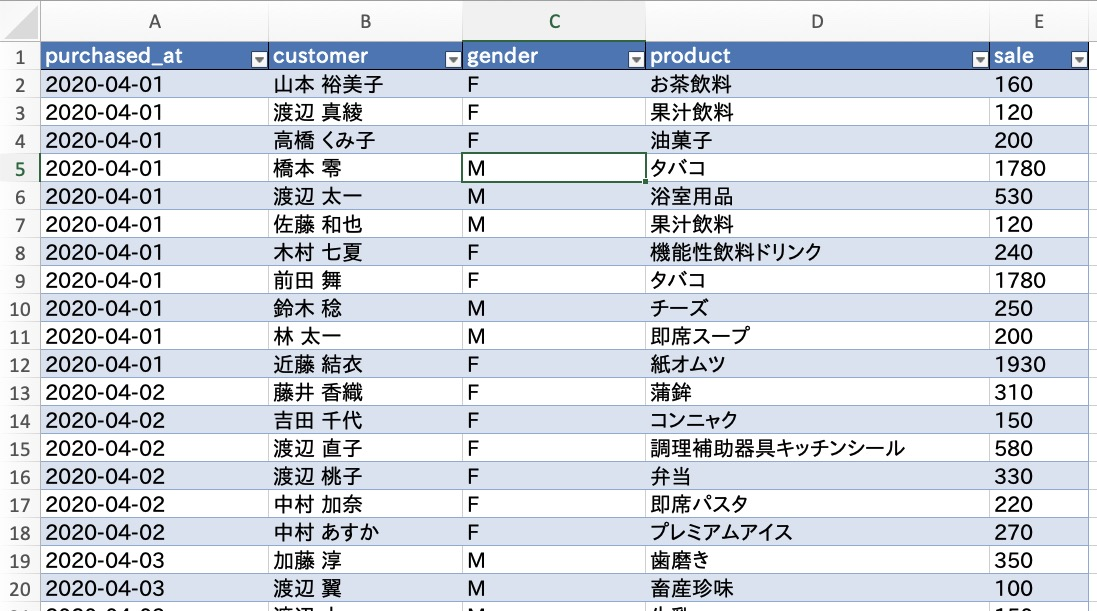
\includegraphics[width=0.9\textwidth]{figure/introduction/yamabata-san-table.jpg}
    \caption{山畑さんが分析に用いた初期のExcelデータの一部．}
    \label{fig:yamabata-san-table}
\end{figure}

図\ref{fig:yamabata-san-table}は，山畑さんが分析の練習材料として用いたExcelデータの一部です．
図を見るとわかるように，このExcelシートでは以下の5項目についてデータが記録されています．
\begin{itemize}
\item \graybox{purchased\_at}: 購買（販売）日時
\item \graybox{customer}: 商品を購入した人物の氏名
\item \graybox{gender}: 商品を購入した人物の性別
\item \graybox{product}: 購入された商品名
\item \graybox{sale}: 販売価格
\end{itemize}

ご存じの通り，Excelはビジネス現場で非常によく使われている表計算ソフトです．
そのすべてを理解している人は少ないですが，データの絞り込みや集計など，便利な機能がたくさん備わっています．
ここでは，山畑さんになりきって以下のクイズに取り組んでみてください．
どのクイズも，販売履歴データの分析においてはよくあるタスクです．


\subsubsection{Q1-購買頻度：あの人は何回買い物をしている？}
Excelの検索機能を用いて，「岡田 真綾」という人物が何回買い物をしていたかを数えてください．

\subsubsection{Q2-購入者の絞り込み：商品Xを購入しているのは誰？}
Excelのオートフィルタ機能を用いて，「ビタミン補助剤」を購入している人をリストアップしてください．

\subsubsection{Q3-総売上金額}
Excel関数の\graybox{\texttt{SUM}}を用いて，現時点での総売上金額を計算してください．

\subsubsection{Q4-人気商品：最も売れた商品は？}
Excelの「ピボットテーブル」機能を使って，集計期間中に
\begin{itemize}
\item 最も購買回数が多かった商品
\item 最も売上金額の合計が大きかった商品
\end{itemize}
をそれぞれ求めてください．

\vspace{2zw}
いかがでしたでしょうか．
Excelの基本的な機能を使えば，どのクイズもサクっと解けたのではないでしょうか．

Excelはビジネス上計算に必要な機能が一通り備わっています．
なにより，大抵のPCにはインストールされているオフィスツールですから，手軽に使えるのが魅力です．
学術研究の世界でも，データの簡単な集計や可視化にはしばしばExcelが使われます．

何も問題がないように見えるExcelですが，扱うデータの規模や用途が大きくなると，様々な問題に遭遇します．
山畑さんのその後の話を例に，その問題点を一緒に考えてみましょう．


% ---------------------------------------
\section{ケース2: サイトの認知度向上につき，得られるデータも膨大に!?}
% ---------------------------------------
現時点では手持ちのデータは少ないものの，販売履歴データの分析に将来性を感じた山畑さん．
販売履歴データを有効活用できるよう，ショッピングサイト運営により力を入れる決意を固めたのでした．

以下は，山畑さんのその後の話（架空の話）です

\begin{framed}
ショッピングサイト立ち上げ以降，順調に利用者数も増えていった．
やはりメディアに取り上げられたのが大きかったのだろう．
あのタイミングでサイトの認知度が一気に高まり，サイトの利用者数や利用頻度も加速度的に増えていった．
それに伴い，サイト運営に関わるスタッフも増員した．

販売履歴の管理は，当初は山畑さんが一人で担当していたが，さすがに一人では対応しきれなくなった．
そこで，ある時点から数名体制で販売履歴の記録を行うことになった．
これまで販売履歴の管理に使ってきたExcelシートをクラウドストレージに置き，記録担当スタッフのPC間で同期を取る仕組みを導入．
同じExcelファイルの上で，スタッフ全員で販売履歴を記録できるようにしたのである．

2年後．サイト事業は軌道に乗った．
十分な量の販売履歴データが蓄積されたと判断した山畑さんは，いよいよ大規模な販売履歴データの分析に取りかかることを決意した．
立ち上げ当初は200〜300行しかなかったExcelシートであったが，シートを開きその行数を数えてみると・・・
なんとその数90万行以上！
データの量に小躍りした山畑さんは，Excelシートの扱いに詳しいスタッフと共に，意気揚々とデータ分析に取りかかったのであった．
\end{framed}

オンラインショッピング事業に成功した山畑さん，蓄積された販売データも膨大な量になりましたね．
90万行以上もあるExcelシートは，まさに「巨大なデータのかたまり」になっています．

さあ，ここからは再度，山畑さんになりきってこのExcelシートを用いたデータ分析に取り組んでみましょう．
こちらのURL（\url{https://github.com/trycycle/database-textbook/raw/refs/heads/main/dataset/purchase\_large.xlsx}）には，上記ケース2で山畑さんが分析しようとしているExcelファイルがあります\footnote{繰り返しになりますが，データはすべて架空のものです．}．
まずは，そのExcelファイル（\graybox{purchase\_large.xlsx}）をダウンロードし，ファイルを開いてください．
このExcelファイルのシートは，先ほどのケース1で用いたExcelシートと同じ構造（項目）となっています．
異なるのは，データの量（行数）だけです．
もし，ファイルがうまく開けない場合は，こちらのURL（\url{https://github.com/trycycle/database-textbook/raw/refs/heads/main/dataset/purchase\_medium.xlsx}）からダウンロードできるExcelファイル（\graybox{purchase\_medium.xlsx}）を用いてください．
ダウンロードが完了したら，ケース1と同じタスク（Q1〜Q4）に取り組んでみてください．
同じタスクでもデータが増えたことで異なる結果が得られるでしょうし，別の体験が得られるはずです．


% ---------------------------------------
\section{表計算ソフトでデータ管理を行ったときに起きる悲劇}
% ---------------------------------------
ケース1および2で用いたExcelファイルは，販売履歴データの集まりでした．
一般的には，このようなデータの集まりは「データベース」ということになるでしょう．

ところで，ケース2のタスクに取り組んでみて，イライラを感じたりしませんでしたか．
実はケース2のExcelファイルには，大量のデータを管理・処理する上での課題を感じていただくために，いくつかの問題を仕込んでおきました．

ファイルを開いた方がまず感じたのは，Excelの動作が重い，ということでしょうか．
Excelは，基本的にデータをすべてメモリに読み込もうとします．
PCのメモリは作業用机のようなものです．
メモリという机が広いほどたくさんの資料（データ）を開いて作業ができますが，机の広さを超えるデータ量を扱おうとすると，PCは身動きが取れなくなってしまいます．
ケース2で扱ったExcelシートは一般的な利用では扱わない量のデータが含まれているため，スペック（メモリ）がそれほど高くないPCを使っている場合，Q1からQ4のタスクに取り組むどころか，Excelファイルを開くことも難しいかもしれません．

無事Excelファイルを開くことができたとしても，ケース2のExcelファイルのデータを分析するには骨が折れます．
まずケース1に比べ，行数が圧倒的に多いです．
そのため，Q1タスクでは，Excelの検索機能を使って「岡田 真綾」さんの行を検索するにしても，データが多すぎて何度も「Enterキー」を押す羽目になります（しかも何回押したか分からなくなる）．
また，ケース2のExcelデータにはデータの誤記や不適切なフォーマットが混入しています．
たとえば，\graybox{sale}の列に半角数字と全角数字が混在しています\footnote{一般に，計算機は半角文字（例: 123，ABC）と全角文字（例: １２３，ＡＢＣ）を区別します．}．
\graybox{purchased\_at}列の日付は，「年\/月\/日」というフォーマットのデータもあれば，「年-月-日」というフォーマットのデータが混在しています．
そのため，Q3タスクでは，売り上げ金額の正しい合計値が得られません（\graybox{SUM}関数は全角数字を無視する）．
さらに，\graybox{product}列では「セル（マス目）1つにつき商品1つ」となっておらず，ある顧客が同時に複数の商品を購入した場合，1つのセルにカンマ区切りで複数の商品が登録されてしまっています．
そのため，Q4タスクではピボットテーブルを使っても，商品ごとの集計が行えなくなっています．

なぜ，このような問題が起きたのでしょうか．
それは，本来Excelは個人用の表計算アプリケーションであって，大規模データの管理や処理を前提として設計されていないためです．
ビジネスの現場で扱うデータは，個人で扱うそれと比べて規模が大きく，多様になることが多いです．
また，複数人，複数部署，複数サービスでデータを共有することも珍しくありません．
そのため，誰かが編集中のデータを別の人が意図せず上書きをしようとしたり，データのフォーマット（形式）や事前に定めた入力ルールを無視してデータを入力してしまう，といった問題も起きやすくなります．
このように，数十万行，数百万行ある表データをExcelで管理・処理しようとすると，さまざまな不都合が生じます（図\ref{fig:excel-disaster}）\footnote{数十万，数百万行の表データはExcelで扱うには大規模ですが，本書で学ぶデータベースシステムにとっては小規模です．現代のデータベースでは，何千万，何億行という規模の表データを扱うことは珍しくありません．}．



\begin{figure}[h]
    \centering
    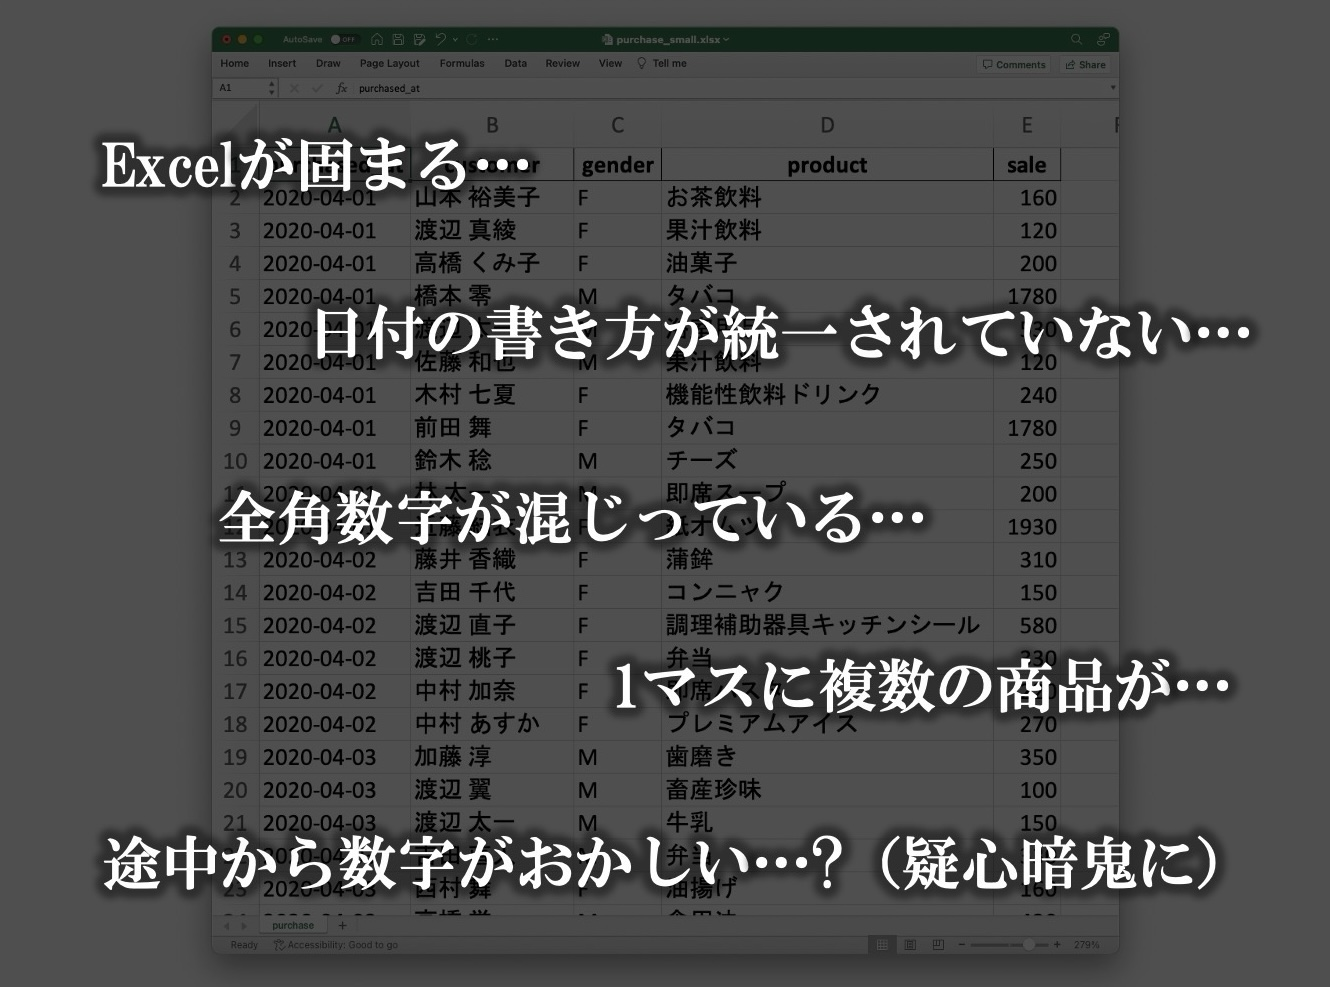
\includegraphics[width=0.8\textwidth]{figure/introduction/excel-disaster.jpg}
    \caption{大きな表データを複数人でExcelで扱うときの悲劇．}
    \label{fig:excel-disaster}
\end{figure}

今日，企業や組織が扱うデータの量はますます増加しています．
また，蓄積された大規模なデータを分析して，ビジネスに活かそうとする動きも活発化しています．
では，大規模なデータをうまく管理・処理するためにはどうすればよいでしょうか．
そのための技術こそが「データベース」です．
「データベース」を用いれば，不適切なデータが混入することを防いだり，大量のデータを効率よく検索・集計することが可能になります\cite{Astrahan1976}．
以降，本書では\strong{大規模データを効率よく管理・処理するための「データベース」技術} について解説します．


\chapter{データベースの基礎知識}\label{chap:concept-of-database}
今日，データベースは様々な業務やアプリケーションで利用されています．
例えば，Amazon\footnote{Amazon．\url{https://www.amazon.co.jp/}}や楽天市場\footnote{楽天市場．\url{https://www.rakuten.co.jp/}}といったオンラインショッピングサイトにおいては，購買履歴管理や在庫管理を行うためにデータベースが用いられています．
Instagram\footnote{Instagram．\url{https://www.instagram.com/}}やTiktok\footnote{Tiktok．\url{https://www.tiktok.com/}}といった，多数のユーザがコンテンツを投稿・閲覧するソーシャルメディアにおいてもデータベースは欠かせません．
個人用ブログのような比較的小規模なウェブサイトでも，記事データを管理するためにデータベースが用いられています（例: WordPress\footnote{WordPress．\url{https://ja.wordpress.org/}}．
このように，データを語る上でデータベースはなくてはならないものです．

本章では，データベースの概念を説明した後，最も代表的なデータベースであり，かつ本書の主要テーマでもある\strong{関係データベース}の概要について述べます．


% ---------------------------------------
\section{データベースとは}
% ---------------------------------------
データを収集・利用する文化が根付いてきたこともあり，データベースという言葉が市民権を得つつあります．
しかし，「データベース」という語が指す意味は，一般人とITの専門家とは大きく異なります．
第1章でも述べたように，一般の方にとってのデータベースとは「データの集まり」くらいの意味で捉えられていることが多いです\footnote{データと情報も明確に区別されることなく使われることが多いですが，情報学の世界では区別されています．データは「様々な活動や営為の結果得られる記号の集まり」であり，情報は「データが解釈され，意味や価値が付加されたもの」を指します．}．
一方，ITの専門家にとってのデータベースは，
\begin{quote}
``複数の応用目的での共有を意図して，組織的にかつ永続的に格納されたデータ群（北川博之著「データベースシステム」\cite{北川本}より）''
\end{quote}
あるいは
\begin{quote}
``データの正しさを管理する主体によって体系的に整理され，計算機によって永続的に格納されたデータの集まり（吉川正俊著「データベースの基礎」\cite{吉川本}より）''
\end{quote}
を意味します．
「データの正しさを組織的に管理する」という考えが強調されています．

データベースを扱うためのシステムは，\strong{データベース管理システム（database management system, DBMS）}と呼ばれます．
我が国のデータベース研究の大家である増永良文氏はその著者の中で，データベースとDBMSの関係を「料理」と「それを盛る器（うつわ）」の関係に例えています\cite{増永本}．
\begin{itemize}
\item データの正しさを組織的に管理するための「器」がDBMS
\item DBMSという器に盛られた「料理」，すなわち正しく管理されたデータの集まりがデータベース
\end{itemize}
という対応関係になります．
本来データベースとはDBMSによって管理されるデータ群を指しますが，データ管理の現場では，DBMSそのもの（あるいはDBMSとそれによって管理されるデータ群）をデータベース（DB）と呼ぶこともあります．

増え続ける多様かつ大量のデータと付き合っていくためには，データの\.う\.ま\.い管理・処理方法が必要になります．
場当たり的にデータを作ってはファイルとしてフォルダ（ディレクトリ）に突っ込んでおいたり，Excelシートにまとめていくというやり方は，扱うデータが増え，データを使う人間やアプリケーションが増えるにつれて，やがて破綻します．
ITの専門家が考えるデータベースは，こういった事態を未然に防ぐための強力なツールとなります．


% ---------------------------------------
\section{大規模なデータを扱う上での課題}
% ---------------------------------------
第1章の山畑さんの事例で見たように，大量のデータを適切かつ効率的に管理・処理するには，以下のような要件が求められます．

\subsubsection{多様かつ大規模なデータの管理}
ビジネスをはじめとする現場では，多種多様かつ大量のデータが時々刻々と発生しています．
例えば，2020年1月1日から2020年12月31日までの12か月間に，Amazon.co.jpで購買された商品の数は5億点以上にのぼるとされています\cite{DataVolumeOfAmazon}．

個人で管理する家計簿のような小規模な表データであれば，Excelのような表計算ソフトでも対応できます．
しかし，データの規模が大きくなり，様々な種類のデータが登録されるようになり，表データの登録・更新に関わる人が増えていくと…
やがてデータの管理が破綻するのは想像に難くありません．
何がどこに登録されているのかもよく分からなくなりますから，目当てのデータを探すのも大変です．
データの登録，修正，削除などなど，何をするのも大変になります．

そもそもExcelは1つの表につき最大100万行程度しか扱えません．
Excelのようなスプレッドシートでは，購買データのように数千万行，数億行もある多様かつ大規模なデータを効率よく蓄積，管理することは困難極まりないのです．


\subsubsection{データの正しさの保証}
管理するデータが大量かつ多様になってくると，データを正しく保つことが難しくなってきます．
特に，大量のデータを複数人，複数のグループや部署で扱うようになると，データの入力ミス，データ入力規則の無視，データ間の矛盾が発生しやすくなります．

当然ですが，管理対象となるデータに誤りが混入すると，そのデータを使うときに大変なことになります．
例えば，図\ref{fig:bad-data}のように，購買データの中に
\begin{itemize}
\item 現実にはあり得ない売り上げ金額が記録されている（データの入力ミス）
\item 入力形式が異なる日付が混在している（データの入力規則の無視）
\item 取扱商品リストにないはずの商品が購買履歴に含まれている（データ間の矛盾）
\end{itemize}
といったことが起きると，オンラインショッピング事業においては一大事です．
このような正しくないデータは直接参照されたときも問題になりますが，複数のデータを集計する際にも悪影響を及ぼします．
それゆえ，データ管理においては，格納されるデータの正しさ，データ間の矛盾のなさを保証する機能が求められます．

\begin{figure}[h]
    \centering
    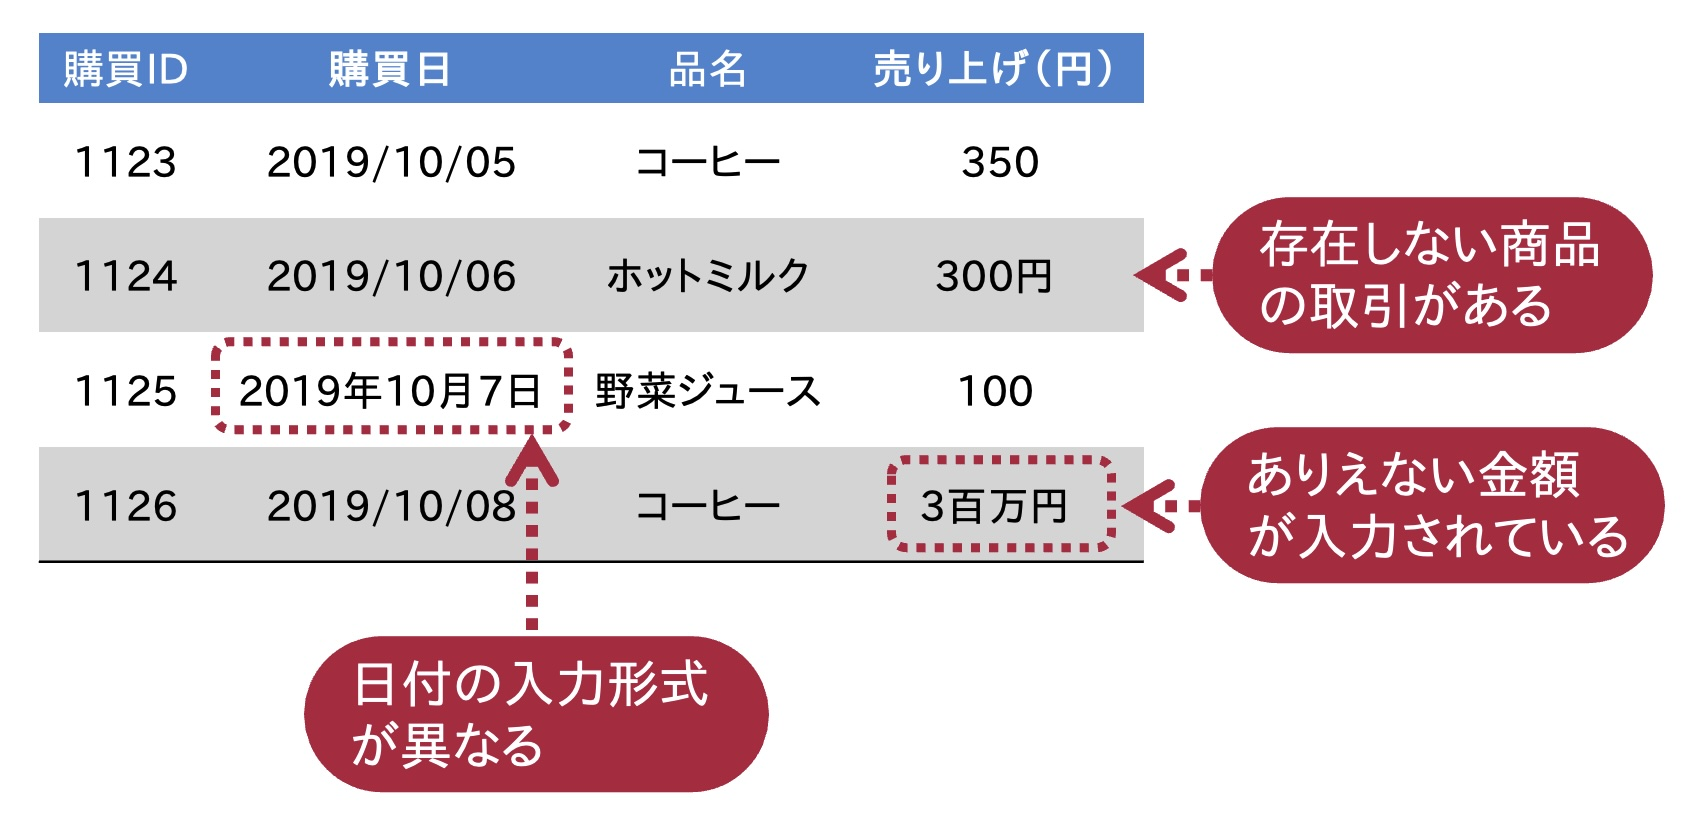
\includegraphics[width=1.0\textwidth]{figure/concept-of-database/bad-data.jpg}
    \caption{正しくないデータの例．}
    \label{fig:bad-data}
\end{figure}


\subsubsection{高速で効率的なデータ処理}
大量のデータを正しく管理できたとしても，対象となるデータを高速に処理できなければ実用的ではありません．
例えば，図書館における書籍の検索システムを考えてみよう．
たとえ数百万件の書籍情報を正しく管理する蔵書管理システムがあっても，ニーズにマッチする書籍のリストの検索に数分待たされるようでは，誰も使いたくありません．

一般に，あるシステムを利用するユーザが増えるにつれて，システムにかかる負荷も増えていきます．
例えば，Amazon.co.jpでは毎分平均900件以上の商品取引が行われています\cite{TransactionInAmazon}．
それゆえ，大量のデータが格納されているシステムにおいては，多発的に大量のデータのやりとりが発生することも想定して，高速かつ効率的なデータ処理が求められます（図\ref{fig:linear-search-for-table}）．

\begin{figure}[h]
    \centering
    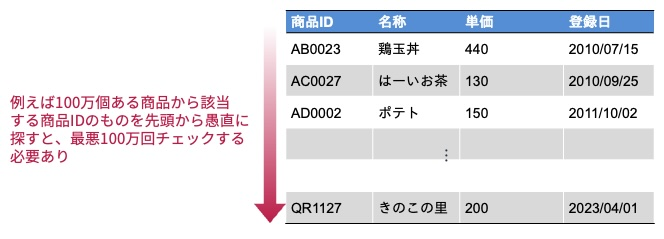
\includegraphics[width=1.0\textwidth]{figure/concept-of-database/linear-search-for-table.jpg}
    \caption{上から下に順に調べ上げていく線形探索では．大規模データに対する高速なアクセスは難しい．}
    \label{fig:linear-search-for-table}
\end{figure}


\subsubsection{同時実行（並列処理）}
関連して，大勢の人が同時にデータを追加，更新，削除しても，管理中のデータに矛盾が生じないようにシステムが動作することも重要です．

例えば，Xさん，Aさん，BさんがPoyPoyという名称のコード決済システムを利用しているとしましょう．
最近のコード決済システムはお店にお金を支払うだけでなく，ユーザ同士でお金を送金しあうこともできます．
さて，XさんのPoyPoy口座残高は5万円とします．
一般に，口座への送金があった際，送金先口座の残高の計算は
\begin{quotation}
残高 = 送金時の「送金先口座」の残高 + 送金額
\end{quotation}
送金元口座の残高の計算は
\begin{quotation}
残高 = 送金時の「送金元口座」の残高 - 送金額
\end{quotation}
となります．
これは至極当然の処理ですが，次のような状況を考えてみましょう．

ある日，Xさん，Aさん，Bさんは食事に出かけ，XさんがAさん，Bさんの代金を立て替えたとします．
AさんとBさんは，PoyPoyアプリを通じてXさんに立て替えてもらった金額（3000円）を精算することにしました．
さて，AさんとBさんは，XさんのPoyPoy口座に\strong{まったく同じタイミングで}3000円送金したとします．
この際，前述の計算式をそのまま適用すると，図\ref{fig:mutual-exclusion}のように誤った処理が行われてしまいます．
\begin{figure}[tb]
    \centering
    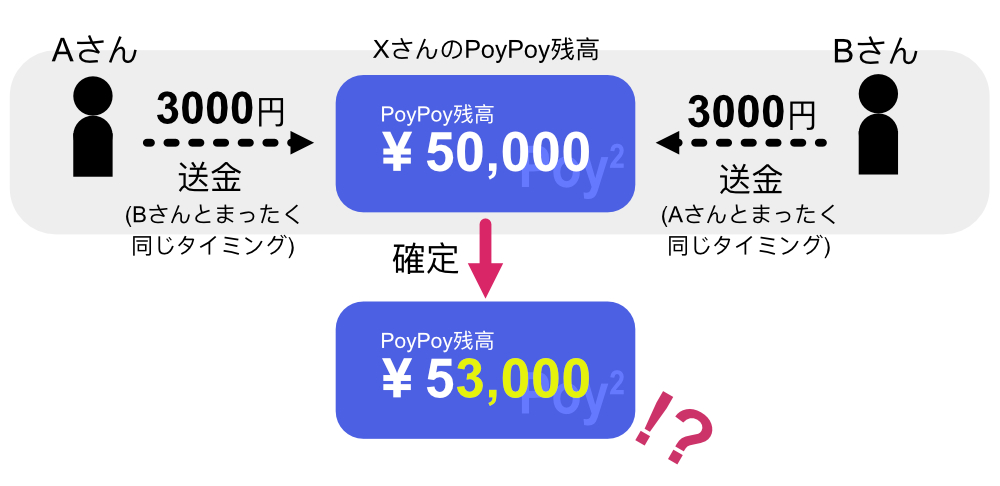
\includegraphics[width=0.8\textwidth]{figure/concept-of-database/mutual-exclusion.jpg}
    \caption{複数の処理要求を矛盾なく処理できていない例．}
    \label{fig:mutual-exclusion}
\end{figure}
AさんとBさんが送金を行った後，Xさんの口座の残高は5万3000円になりました -- こんなことが起きたら大変ですよね．
この例における問題点は，たとえ振込み処理が同時に発生したとしても，Aさんの振り込み処理を待ってからBさんの処理を行うべきであったという点です．

このように，データ処理の内容によっては，別の処理が完了したことを保証してから次の処理を行う必要があります．
さらに，処理の途中で何らかのエラーが起きた場合は，すべての処理をキャンセルして最初の状態に戻すことが求められます．
データを管理しているシステムに同時アクセスがあった場合でも，データを矛盾なく処理できることが重要となります．


\subsubsection{アクセス権限のコントロール}
データによっては，誰でも自由に閲覧してよいものもあれば，特定の立場のユーザしかアクセスできないようにすべきものも存在します．
多種多様なデータのやりとりが発生する環境においては，ユーザの属性ごとにデータの閲覧，作成，更新，削除といったアクセス権限を制御する機能が必要となります．


% ---------------------------------------
\section{データベースを用いるメリット}
% ---------------------------------------
一人で扱えるほどデータの規模が小さければ，Excelなどの表計算用のソフトウェアでデータ管理しても問題はありません．
しかし，扱うデータが多様かつ大規模になると，問題が生じなくするために要求されるデータ処理の質が変わります．
そのため，データの管理方法や処理方法を見直す必要があります．

本稿で学ぶデータベースを用いれば，\strong{データの一元管理}が可能となり，データの管理や利活用において様々な恩恵を受けられます．
具体的には，データベースが備える以下のような特性あるいは関連技術を用いることで，前節で述べた「大規模なデータを扱う上での課題」をクリアすることができます．
\begin{itemize}
\item 大規模なデータの管理：「\strong{物理的データ格納方式}」の工夫によって対応
\item データの正しさの保証：「\strong{一貫性制約}」によって対応
\item 高速で効率的なデータ処理：「\strong{索引づけ}」「\strong{問い合わせ最適化}」などで対応
\item 同時実行，データの共同利用：「\strong{トランザクション}」などで対応
\item アクセス権のコントロール：「\strong{ロール管理}」によって対応
\end{itemize}



% ---------------------------------------
\section{関係データベース超入門}
% ---------------------------------------
これから本書で学ぶ\strong{関係データベース（relational database）}とは，あらゆるデータを\strong{表（table）}\footnote{表のことをテーブルと呼ぶこともある．}の形式で管理するデータベースです\cite{Codd1970}．
第3章で述べるように，実はデータベースといっても様々な種類のものがありますが，関係データベースはその中でも最も代表的なものです．
関係データベースを管理するためのシステム（すなわちDBMS）は，\strong{関係データベース管理システム（relational database management system，略してRDBMS）}と呼ばれています．

\begin{figure}[h]
    \centering
    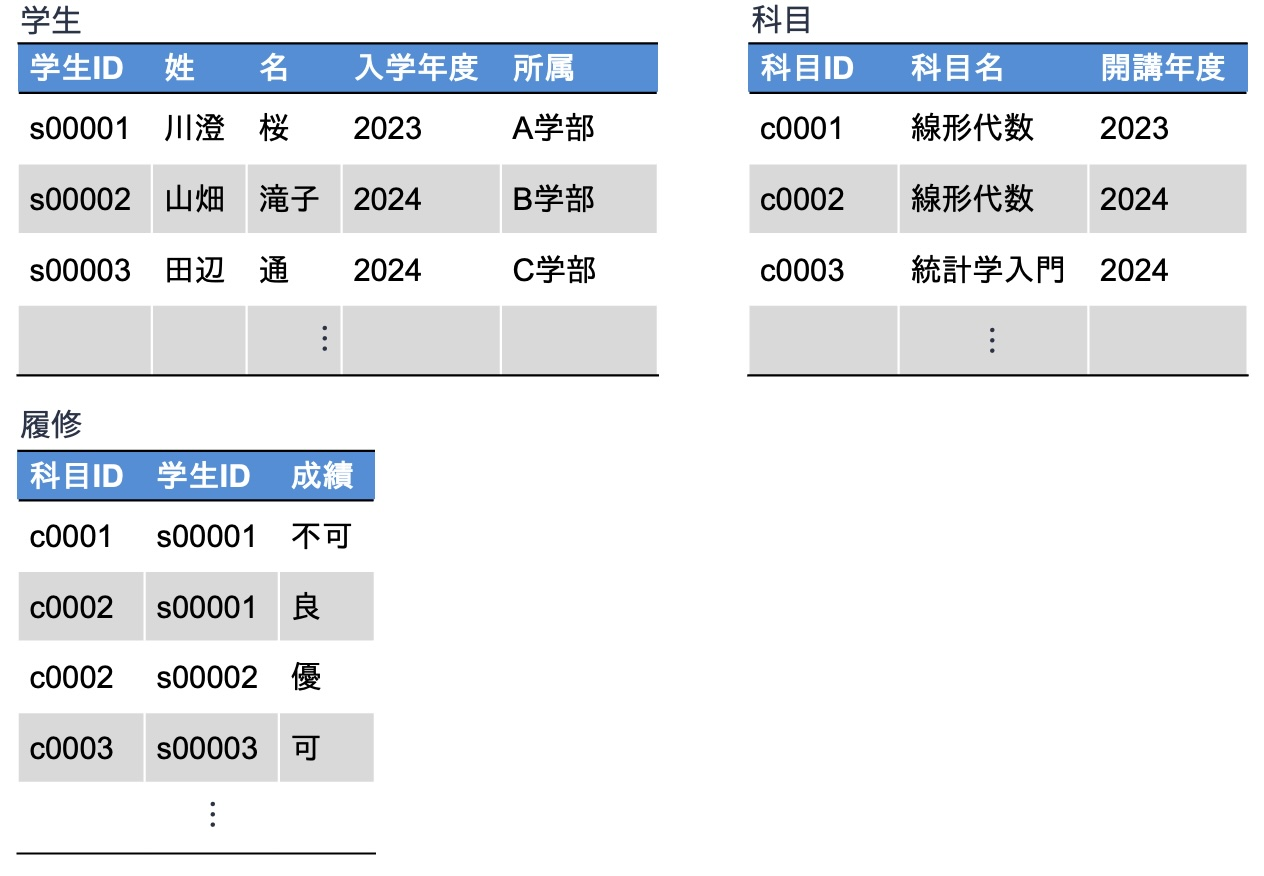
\includegraphics[width=1.0\textwidth]{figure/concept-of-database/example-of-relation.jpg}
    \caption{関係データベースの例．}
    \label{fig:example-of-relation}
\end{figure}

図\ref{fig:example-of-relation}は，授業の履修状況・成績を管理する関係データベースの例です．
この関係データベースには，以下の3つの表が存在しています．
\begin{itemize}
\item 学生テーブル：学籍番号，氏名，入学年度，所属といった学生に関する情報を格納
\item 科目テーブル：科目ID，科目名，開講年度といった科目に関する情報を格納
\item 履修テーブル：どの学生が何の科目を履修し，どのような成績であったかに関する情報を格納
\end{itemize}
各表は行と列から構成されており，各行には表が扱うデータが格納されています．
図\ref{fig:example-of-relation}の学生テーブルを例に取ると，各行のデータは学生一人一人の情報を表しています．
関係データベースでは，行のことを\strong{タプル（tuple）}あるいは\strong{レコード（record）}と呼びます．
各レコードは，表の見出しに対応するデータの値を持ちます．
各見出しのことを\strong{属性（attribute）}，属性に対応するレコードの値を\strong{属性値（attribute value）}と呼びます．
学生テーブルの例では，学生ID，姓，名，入学年度，所属が属性に対応し，一番上に書かれているレコードの属性「学生ID」の属性値は\graybox{s00001}となっています．

この例だけ見ると「なんだ，関係データベースは単なる表じゃないか」と思われたかもしれませんが，\strong{ただの表ではありません}．
一見するとただの表にしか見えませんが，データを正しくかつ効率よく管理・処理するために，あらかじめ定義された「データの構造」「データの制約」「データの操作」に関する規則に従ってデータが作られ，関係データベース内に格納されます\footnote{データの構造，制約，操作に関する規則を定めたものを「データモデル」と呼びます．データモデルについては，第3章で詳しく述べます．}．
例えば図\ref{fig:example-of-relation}の関係データベースであれば，以下のような規則に従い，授業の履修状況や成績を管理するための情報が複数のテーブルに分割され，データベース内に格納されています：
\begin{itemize}
\item 学生テーブルは「学生ID」「姓」「名」「入学年度」「所属」という属性をもつ
\item 学生テーブルの「学生ID」や科目テーブルの「科目ID」はテーブル内で値が重複することはない
\item 履修テーブルには，科目名や学生の氏名といった科目や学生の詳細情報は格納しない
\item 履修テーブルの成績には「優」「良」「可」「不可」のいずれかしか登録できない
\item 履修テーブルに現れる科目IDおよび学生IDは，必ず学生テーブルと科目テーブルに存在する
\end{itemize}

少し詳しく見てみましょう．
図\ref{fig:primary-key}のように，学生テーブルの「学生ID」は重複することがないため，その値が決まれば学生の情報が一意に決まります（どの学生かが特定できる）．
このような属性（またはその組み合わせ）テーバーン委データベースでは\strong{主キー（primary key）}と呼びます．

\begin{figure}[h]
    \centering
    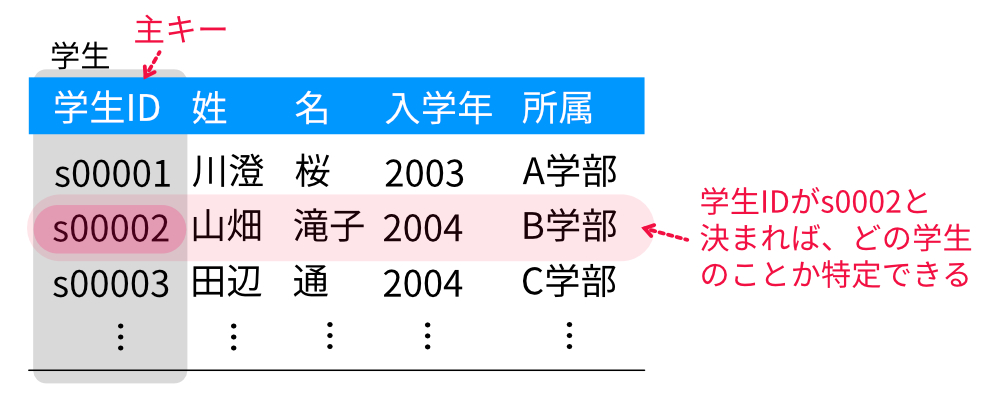
\includegraphics[width=0.8\textwidth]{figure/concept-of-database/primary-key.jpg}
    \caption{主キーの役割}
    \label{fig:primary-key}
\end{figure}

履修テーブルはどの学生が何の科目を履修し，どのような成績であったかを管理するための表ですが，学生の具体的な情報は保持せず，学生IDのみを保持しています．
学生の姓や名，所属といった情報が欲しい場合は，学生IDを手がかりに学生テーブルを参照すれば取得できます．
同じことは科目情報についても言えます．
これは見方を変えると，履修テーブルに格納された学生IDや科目IDは，必ず学生や科目の詳細情報を参照できるよう，必ず学生テーブルや科目テーブル内に存在している必要がある，ということになります．
このように，他のテーブルでは主キーとなっていて，それを手がかりにすることで関連情報を参照するための属性を，関係データベースでは\strong{外部キー（foreign key）}と呼びます．
図\ref{fig:foreign-key}の例では，履修テーブルにおける学生IDや科目IDは（学生テーブルや科目テーブルに対する）外部キーとなっています．
（直感的なイメージとしては）外部キーは，ウェブページにおけるハイパーリンクのような役割を果たしています．
先の例で言えば，履修テーブルの学生IDをクリックすると，学生テーブルから該当学生の詳しい情報が見れる，といったイメージです．
このような仕組みによって，関係データベースは情報が冗長にならないように整理整頓されています．

\begin{figure}[h]
    \centering
    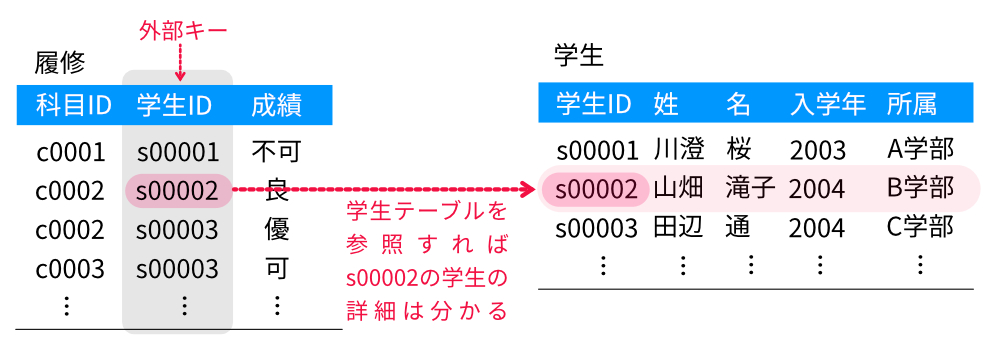
\includegraphics[width=1.0\textwidth]{figure/concept-of-database/foreign-key.jpg}
    \caption{外部キーの役割}
    \label{fig:foreign-key}
\end{figure}

なぜ履修テーブルに学生や科目の詳細情報も載せないのでしょうか．
それは，学生や科目の詳細情報が変更された場合に，履修テーブル内の情報もすべて更新しなければならなくなるからです．
もしすべての情報を1つの表にまとめていたら，どうなるでしょうか．
例えば，山畑さんが在学中にB学部からD学部に転部し，所属が変わったとしましょう．
この場合，もし履修テーブルに山畑さんに関する情報が100件登録されていたら，100件すべての所属をB学部からD学部に書き換えなければなりません．
その際，もし1件でも書き換え忘れがあったら，B学部の山畑さんとD学部の山畑さんが混在することになり，正しい成績証明書が出せなくなってしまいます．
図のように，学生や科目の詳細情報を履修テーブルとは別のテーブルに分けておけば，学生や科目の詳細情報が変更された場合でも，学生テーブルや科目テーブル内の情報を1か所更新すれば済みます．
このような工夫も，関係データベースの重要な特徴の1つです．

上記のような工夫はデータの正しさを保証するためのものでしたが，他にも関係データベースにはデータの検索・集約を効率よく行うための仕組みや同時アクセスの制御など，データを適切に扱うための様々な仕組みが備えられています．
次章以降では，
\begin{itemize}
\item 一見ただの表にしか見えない関係データベースが，どのような理論に基づいて定式化されているか
\item 関係データベースをどのように設計するのか
\item 関係データベースを用いると，なぜ大規模データの管理が効率的になるのか
\end{itemize}
などについて詳しく述べていきます．


% ---------------------------------------
\hrulefill
\section{クイズ}
% ---------------------------------------
\subsubsection{Q1. メジャーなデータベース管理システム}
ウェブ検索エンジンを用いて，世の中にあるメジャーなデータベース管理システムを調べなさい．
また，調べたデータベース管理システムを「関係データベースを扱うもの」と「そうでないもの」に分類しなさい．

\subsubsection{Q2. 線形探索}
100万件ある商品リストの中に特定の商品が含まれているかを確認したいとします．
商品リストの先頭から末尾まで順に商品名を確認していくと，平均で何回（何件）の確認で商品の有無を確認できるでしょうか．

\subsubsection{Q3. データベース管理システムの利用例}
普段利用しているサービスのうち，データベース管理システムを用いていると思われるものを3つピックアップしなさい．

\subsubsection{Q4. CSV/TSVファイル}
CSVファイルおよびTSVファイルとは何かを調べなさい．
また，（データベース管理システムでデータを管理する場合と比較して）CSV/TSVファイルに存在する欠点を挙げなさい．

\subsubsection{Q5. チューリング賞}
関係データベースの理論的基盤である関係モデルを提唱したEdgar F. Codd氏は，計算機科学分野のノーベル賞といわれるチューリング賞の受賞者である．
Codd氏以外で，データベースに関する功績でチューリング賞を受賞した人をピックアップしなさい．

\chapter{関係データモデル}\label{chap:relational-data-model}

\strong{関係データベース（relational database）} とは，関係データモデルにもとづき表現されたデータの集まりである．
関係データモデルは，最も代表的なデータモデルである．
1970年にEdgar F. Codd氏により提案されたもので，単純ながらその背後には強力な数学的基盤をもつ\cite{Codd1970}．
関係データモデルでは，あらゆるデータを\strong{表（table）}としてモデル化する．
%前章で述べたように，関係データモデルとは，表によってデータを表現するデータモデルである．
一見すると単純な表にしか見えない関係データモデルは数学によって定式化されており，強固な理論的基盤を有している．
関係データモデルを用いることで，データから冗長性を排除し，データを正しく管理することが可能となる．

以下では，数学的な観点から関係データモデルについて述べる．
少々堅い説明にはなるが，関係データベースという計算機科学技術が数学に支えられていることを知るためにも，眠気を我慢して読んでほしい．
なお，本講では数学における「集合と写像」の知識を使う．
%最低限の知識を[コチラ](../misc/math.md)にまとめたので，不安がある方はそちらを参照されたい．



\begin{notebox}{計算機科学とは抽象化の学問}
計算機科学（あるいは情報科学）というと「プログラミングでしょ」と考える学生は多いが，それは間違いである．
計算機科学の本質は，\strong{物事を計算可能な状態にする（抽象化）して，計算機の上で処理・分析}することにある．
データベースもその一つである．
計算機科学は抽象化の学問なのである．
\end{notebox}

% ---------------------------------------
\section{関係データモデルのデータ構造}
% ---------------------------------------
\begin{table}[tb]
\centering
\caption{ある小売店の商品に関するデータを収めた関係}
\label{tab:correct-table}
\begin{tabular}{@{}llll@{}}
商品            &             &             &              \\ \midrule
\textbf{商品ID} & \textbf{名称} & \textbf{単価} & \textbf{登録日} \\ \midrule
P1            & はーいお茶       & 130         & 2020/07/15   \\
P2            & 午前の紅茶       & 130         & 2020/09/25   \\
P3            & 健康麦茶        & 150         & 2021/02/16   \\
$\vdots$      & $\vdots$    & $\vdots$    & $\vdots$     \\
P1000         & きのこの里       & 200         & 2023/01/08   \\ \bottomrule
\end{tabular}
\end{table}

表\ref{tab:correct-table}は，ある小売店で取り扱っている商品のデータを関係データモデルによって表現したものである．
この表において，各行は小売店で取り扱っている商品に対応し，各列には各商品に関するデータが記述されている．

表の左上にある「商品」はこの表の名前を示しており，\strong{関係名}と呼ばれる．
関係データモデル上では，各行は\strong{タプル（tuple）} と呼ばれる．
表の1行目には，「商品」がどのようなデータを持つかを示す見出しが付けられている．
表における各見出しに対応するものを，関係データモデルでは\strong{属性（attribute）}と呼ぶ．
また，各タプルにおけるある属性の値を\strong{属性値}と呼ぶ．
例えば，表中の2行目に対応するタプルは
\begin{equation}
(``P1", ``はーいお茶", 130, ``2020/07/15")
\end{equation}
であるが，このタプルの属性「単価」の属性値は\graybox{130}となる．

% ---------------------------------------
\subsection{数学における「関係」}
% ---------------------------------------
ところで，関係データベースあるいは関係データモデルの「関係」とは一体何だろうか．
\strong{関係（relation）} とは数学上の概念である．
集合$S_1, S_2, ..., S_n$が与えられたとき，それらの直積集合$S_1 \times ... \times S_n$とは

\begin{equation}
S_1 \times ... \times S_n = \{(x_1, ..., x_n) \ | \ x_1 \in S_1, ..., x_n \in S_n \}
\end{equation}
と表現されるものである．
（数学上の概念である）関係とは，このような直積集合の部分集合を意味する．
正確に書くと，集合$S_1, S_2, ..., S_n$が与えられたとき，直積集合$S_1 \times ... \times S_n$の部分集合を$S_1, S_2, ..., S_n$上の\strong{n項関係}と呼ぶ．

例えば，$A=\{2, 3\}$，$B=\{-2, -3\}$が与えられたとき，直積$A \times B$は集合AおよびBの要素のすべての組み合わせであるから

\begin{equation}
A \times B = \{(2, -2), (2, -3), (3, -2), (3, -3)\}
\end{equation}
となる．
このとき，その部分集合の1つである
\begin{equation}
\{(2, -3), (3, -2)\}
\end{equation}
は集合AおよびB上の2項関係となる．
このような（n項）関係の概念を使って，関係データモデルは理論構築されている．


% ---------------------------------------
\subsection{関係データモデルにおける「関係」}
% ---------------------------------------
\strong{関係データモデルにおける関係}は「数学における関係」を拡張したものになっており，以下の2つから構成される．
\begin{itemize}
\item 関係スキーマ
\item インスタンス
\end{itemize}

\strong{関係スキーマ（relation schema）} とは，関係の名前と属性の集合，および（後述する）一貫性制約の情報を示すものである．
関係スキーマは

\begin{equation}
(\boldsymbol{R}(A_1, ..., A_n), \{\sigma_1, \sigma_2, ..., \sigma_m\})
\end{equation}
の形式で記述される．
ここで
\begin{itemize}
\item $\boldsymbol{R}$は関係名
\item $A_1, ..., A_n$は属性
\item $\sigma_1, ..., \sigma_m$は一貫性制約
\end{itemize}
に対応する．
一貫性制約が自明な場合やそれを考慮しないときは，関係スキーマを

\begin{equation}
\boldsymbol{R}(A_1, ..., A_n)
\end{equation}
のように簡潔に表記することもある．
表\ref{tab:correct-table}の関係「商品」の例の場合，関係スキーマは
\begin{equation}
商品（商品ID, 名称, 単価, 登録日）
\end{equation}
と記述する．

関係スキーマに記された各属性には，属性が取り得る値の集合を定義する．
この集合は\strong{ドメイン（domain; 定義域）} と呼ばれ，属性$A$のドメインは$Dom(A)$と記す．
例えば，表\ref{tab:correct-table}の関係「商品」の例では，属性「単価」は金額を表すので，そのドメイン$Dom(単価)$は0以上の整数値が想定される．
これを数学的に記すと，以下のようになる:
\begin{equation}
Dom(単価) = \{ x \ | \ x \in \mathbb{N} \}
\end{equation}

同様に，属性「商品ID」「名称」「登録日」についても，以下のようにドメインを定義できる．
\begin{eqnarray}
Dom(商品ID) = \{ x \ | x \in Pから始まる文字列集合 \} \\
Dom(名称) = \{ x \ | \ x \in 文字列集合 \} \\
Dom(登録日) = \{ x \ | \ x \in 年月日集合（ただし西暦表記） \}
\end{eqnarray}

\strong{インスタンス（instance）} は，関係スキーマ$\boldsymbol{R}(A_1, ..., A_n)$におけるドメイン$Dom(A_1), ..., Dom(A_n)$の直積の部分集合である．
仮にインスタンスを$R$とすると，
\begin{equation}
R \subseteq Dom(A_1) \times ... \times Dom(A_n)
\end{equation}
である．
インスタンスは，前節で説明した数学上の関係に相当する．
また，インスタンス$R$の要素がタプルとなる．

例に戻って，定義と照らし合わせてみよう．
表\ref{tab:correct-table}の関係「商品」の関係スキーマは$商品(商品ID, 名称, 単価, 登録日)$であった．
各属性のドメインの定義も与えたが，その定義から，例えば属性「単価」については
\begin{equation}
Dom(単価) = \{1, 2, 3, .... 10000, .... \}
\end{equation}
のようにあらゆる自然数を取り得る．
また，属性「名称」については
\begin{equation}
Dom(名称) = \{``あ", ``い", ..., ``はーいお茶", ... \}
\end{equation}
のようにあらゆる文字列を取り得る．

各属性の直積$Dom(商品ID) \times Dom(名称) \times Dom(単価) \times Dom(登録日)$には，
\begin{equation}
(``P001", ``こんな商品はありません", 100兆, ``2020/01/01")
\end{equation}
のように，実際に商品情報としてありえないタプルも含めて，様々なタプルが要素として含まれる．
なぜなら，直積とは集合（ドメイン）の要素のすべての組み合わせであるためである．
ドメインの直積の部分集合をインスタンスとすることは，取り得るタプルの候補から実際にデータとして扱われるタプルの集合を選択することに相当する．


\begin{notebox}{タプルは重複が許されない}
一般的に使われる表では，同じ内容を表す行が複数あっても許される．
一方，関係データモデルに基づく表は行，すなわちタプルの重複は許されない．
なぜなら，関係データモデルのインスタンスは（数学的な）集合だからである．
\end{notebox}


% ---------------------------------------
\section{非正規関係と第1正規形}
% ---------------------------------------
関係データモデルにおけるドメインとは属性が取り得る値の集合を意味するが，ドメインの要素はそれ以上分解不可能な値を意味する\strong{原子値（atomic value）} であることを想定している．
原子値の例としては，文字列，整数，実数，真偽値，日付などが挙げられ，どれもデータの基本単位と呼べるものである．
逆に原子値で「ない」例としては，タプルや集合，関係などが挙げられる．
ドメインとして原子値以外の値をとることを許す関係を\strong{非正規関係（unnormalized relation）} と呼ぶ．
逆に，ドメインとして原子値しかとらない関係は\strong{第1正規形（first normal form; 1NF）である} という．

\begin{figure}[tb]
    \centering
    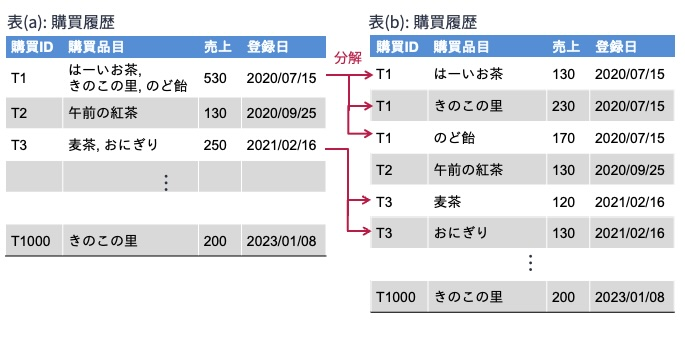
\includegraphics[width=1.0\textwidth]{figure/relational-data-model/unnormalized-relation.jpg}
    \caption{非正規関係}
    \label{fig:unnormalized-relation}
\end{figure}

例えば，図\ref{fig:unnormalized-relation}の(a)(b)はともに商品の購買履歴を表しているが，(a)は属性「購入品目」に集合要素が入ってしまっている（例えば，\graybox{\{``はーいお茶'', ``きのこの里'', ``のど飴''\}}）．
(a)の属性「購入品目」のドメインが原子値以外の値（つまり文字列の集合）を許してしまっていることから，(a)は非正規関係と見なせる．

一方，図\ref{fig:unnormalized-relation}(b)は(a)の購買品目の値が原子値（文字列の集合ではなく文字列）になるように設計されているため，第1正規形と見なせる．
図\ref{fig:unnormalized-relation}(a)では1行で表現できていた1回分の購買データが，(b)では複数行を使って表現されている．
図\ref{fig:unnormalized-relation}(b)のほうがデータ構造が簡潔になるため，データが扱いやすい．


% ---------------------------------------
\section{一貫性制約}
% ---------------------------------------
\strong{一貫性制約（integrity constraint）} とは，データベースが対象とする実世界を反映するように設定された，データが満たすべき規則である．
関係データモデルにおいては，代表的な一貫性制約として以下がある：
\begin{itemize}
\item ドメイン制約
\item キー制約
\item 参照制約
\item データ従属性
\end{itemize}

関係データモデルを扱うデータベースを設計する際には，上記一貫性制約を踏まえて\strong{関係スキーマの定義や（複数の関係スキーマへの）分解} を行う．


% ---------------------------------------
\subsection{ドメイン制約}
% ---------------------------------------
\strong{ドメイン制約（domain constraint）} とは，関係$\boldsymbol{R}(A_1, ..., A_n)$に含まれるタプルの各成分は，対応する属性のドメインの要素でなければならないという制約である．
これは属性の定義ですでに触れたことである．
ドメイン制約では，各属性のドメインのデータ型（例: 整数，実数，文字列，日付）に加えて，値が取り得る範囲を指定することもある．
例えば，

先の例でとりあげた関係
\begin{equation}
商品(商品ID, 名称, 単価, 登録日)
\end{equation}
において，属性「単価」や「登録日」のドメインは
\begin{eqnarray}
Dom(単価) = \{ x \ | \ x \in \mathbb{N} \} \\
Dom(登録日) = \{ x \ | \ x \in 年月日集合（ただし西暦表記） \}
\end{eqnarray}
のように定義されていた．
これらはドメイン制約である．
これら制約にもとづき，
\begin{itemize}
\item 「単価」属性の値は\strong{必ず}自然数
\item 「登録日」属性の値は\strong{必ず}西暦表記の年月日集合
\end{itemize}
でなければならない．
よって，表\ref{tab:incorrect-table}に記した表「商品(*)」の各タプルは関係「商品（商品ID, 名称, 単価, 登録日）」のインスタンスには\strong{なれない}．
なぜなら，
\begin{itemize}
\item 商品IDがP1の商品の登録日は年月はあるが日が抜けている
\item 商品IDがP3の商品の登録日は和暦で表現されている
\item 商品IDがP1000の商品の単価は漢数字（文字列）で表現されている
\end{itemize}
からである．

\begin{table}[tb]
\centering
\caption{ドメイン制約に違反する関係}
\label{tab:incorrect-table}
\begin{tabular}{@{}llll@{}}
商品(*)            &             &             &              \\ \midrule
\textbf{商品ID} & \textbf{名称} & \textbf{単価} & \textbf{登録日} \\ \midrule
P1            & はーいお茶       & 130         & 2020/07   \\
P2            & 午前の紅茶       & 130         & 2020/09/25   \\
P3            & 健康麦茶        & 150         & 令和3年2月16日   \\
$\vdots$      & $\vdots$    & $\vdots$    & $\vdots$     \\
P1000         & きのこの里       & 2百         & 2023/01/08   \\ \bottomrule
\end{tabular}
\end{table}


% ---------------------------------------
\subsection{キー制約}
% ---------------------------------------
まず，キー制約の前提となるキーの概念について説明する．
関係$\boldsymbol{R}$における\strong{超キー（super key）} とは，関係$\boldsymbol{R}$における属性の集合のうち，それらの属性値が決まればおのずと関係$\boldsymbol{R}$のタプルが唯一ひとつに決まる（タプルを一意に特定できる）ものを指す．

例えば，表\ref{tab:contact-relation}は関係スキーマ
\begin{equation}
連絡先(学生ID, 名前, 学年, 大学email, 自宅住所)
\end{equation}
に従うデータを表形式で記したもので，各行（タプル）は学生の連絡先情報を示している．
大学において学生情報を管理する場合，学生ID（の値）が決まれば唯一ひとつの学生連絡先情報（行; タプル）を照会できるよう，学生IDは重複がないように設定される．
それゆえ，この関係「連絡先」において属性「学生ID」は超キーとなる．
同様に，属性「大学email」も超キーとなる．

なお，\{ 学生ID, 名前 \}，\{ 学生ID, 名前, 学年 \} のように学生IDを含む属性の集合も超キーになる．
例えば，「学生ID」が\graybox{S1}，「名前」が\graybox{川澄桜}である行は唯一1行に決まるので，属性集合 \{ 学生ID, 名前 \} も超キーになる．
これは属性「学生ID」が超キーであるから，当たり前である．

一方，属性「住所」は超キーにはなり得ない．
学生IDが\graybox{S3}と\graybox{S4}の学生の住所が同じ（つまり同じところに住んでいる）であるから，住所を1つ指定しても連絡先タプルが一意に特定できないからである．


\begin{table}[tb]
\centering
\caption{関係「連絡先」}
\label{tab:contact-relation}
\begin{tabular}{@{}lllll@{}}
連絡先           &             &             &                    &               \\ \midrule
\textbf{学生ID} & \textbf{名前} & \textbf{学年} & \textbf{大学email}   & \textbf{自宅住所} \\ \midrule
S1            & 川澄 桜        & 4           & kawasumi@xxx.ac.jp & 名古屋市xxx       \\
S2            & 山畑 滝子       & 3           & taki@xxx.ac.jp     & 岡崎市xxx        \\
S3            & 田辺 通        & 3           & t.tanabe@xxx.ac.jp & 尾張旭市xxx       \\
S4            & 田辺 瑞穂       & 1           & m.tanabe@xxx.ac.jp & 尾張旭市xxx       \\
$\vdots$      & $\vdots$    & $\vdots$    & $\vdots$           & $\vdots$      \\
S1000         & 北 千種        & 2           & kita@xxx.ac.jp     & 名古屋市xxx       \\ \bottomrule
\end{tabular}
\end{table}


超キーは複数ありえるが，上の例では属性「学生ID」のみでタプルを特定できるように，属性集合 { 学生ID, 名前 } を使ってタプルを特定しようとするのは無駄であろう．
そこで，超キーのうち極小（つまり最も小さい部分集合）のものを\strong{候補キー（candidate key）} と定義する．
候補キーは単純に\strong{キー（key）} と呼ばれることもある．
例えば，上の関係「連絡先」では，属性「学生ID」や「大学email」が候補キーとなりえる．

最後に\strong{主キー（primary key）} の概念を導入する．
候補キーのうち，値として\strong{未定義や空の値（空値またはNULL値と呼ばれる）} を取る可能性がなく，かつデータベース管理上都合のよいキーの1つを主キーと決める．
主キー以外の候補キーは\strong{代替キー}と呼ばれる．
例えば，先の関係「連絡先」の場合，候補キーは「学生ID」と「大学email」であったが，大学emailは「氏名\@xxx.ac.jp」のようなものから「学籍番号\@xxx.ac.jp」のようなものに変更される可能性があったとしても，学生IDは一度決めたらほぼ変わらないと思われる．
これらを鑑みると，関係「連絡先」においては属性「学生ID」を主キーとして選ぶのがよさそうである．

なお，候補キーの定義から主キーは属性の集合をとることができる．
このような主キーを\strong{複合主キー（composite primary key）} と呼ぶ．
例えば，表\ref{tab:course-completion-relation}は，学生が履修した科目の成績をあらわす関係「履修」を表にしたものである．
この表においては科目IDあるいは学生IDだけでは成績が特定できないが，科目IDと学生IDの両方が決まれば，ある学生のある科目の成績が特定される．
それゆえ，関係「履修」においては \{ 科目ID, 学生ID \} の属性ペアが主キーとなる．

\begin{table}[tb]
\centering
\caption{関係「履修」}
\label{tab:course-completion-relation}
\begin{tabular}{@{}lll@{}}
履修            &               &             \\ \midrule
\textbf{科目ID} & \textbf{学生ID} & \textbf{成績} \\ \midrule
C1            & S1            & 不可          \\
C2            & S1            & 良           \\
C2            & S2            & 優           \\
C3            & S3            & 可           \\
$\vdots$      & $\vdots$      & $\vdots$    \\ \bottomrule
\end{tabular}
\end{table}

関係表と主キー，候補キー，超キーの関係は，図\ref{fig:key-concept-mapping}のようにまとめることができる．
\begin{figure}[tb]
    \centering
    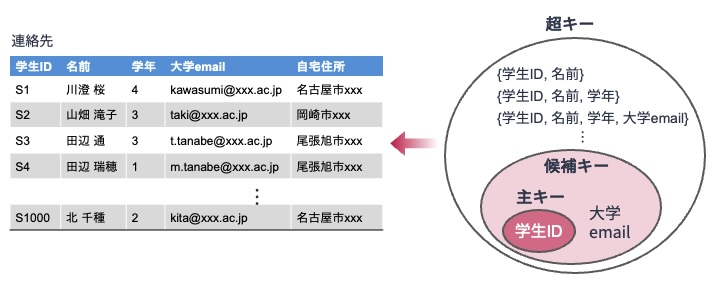
\includegraphics[width=1.0\textwidth]{figure/relational-data-model/key-concept-mapping.jpg}
    \caption{キーの概念の整理}
    \label{fig:key-concept-mapping}
\end{figure}

ここまで，超キー，候補キー，主キーの説明を行ったが，最後に本節の主題であるキー制約について述べる．
\strong{キー制約（key constraint）} は，関係$\boldsymbol{R}$の関係スキーマに対して主キーが設定されたとき，$\boldsymbol{R}$のインスタンスにおいて
\begin{itemize}
\item 主キーに設定された属性の値は重複があってはならない，かつ
\item その要素（タプル）は主キーによって一意に特定されなければならない，かつ
\item 主キーとなる属性の値は\strong{NULL値} であってはならない
\end{itemize}
という制約である．
定義は小難しく見えるかもしれないが，キー制約は「ある属性が主キーと設定されたら，それがきちんと主キーの役割を果たすようデータが作られなければならない」ということを意味している．
主キーを定義できれば，キー制約を定義できたようなものである．

さて，関係スキーマにおいてキー制約以外の一貫性制約には注目しない場合，関係スキーマでは主キーは以下のように下線を引いて表す．
\begin{equation}
\boldsymbol{R}(\underline{A_1, A_2}, ..., A_n)
\end{equation}
例えば，図\ref{fig:key-concept-mapping}の関係「連絡先」であれば，その関係スキーマは以下のように表す．
\begin{equation}
連絡先(\underline{学生ID}, 名前, 学年, 大学email, 自宅住所)
\end{equation}

\begin{notebox}{キーは関係スキーマに対して設定される}
キーは，関係データベース内にあるタプル（行）だけを見て決めてはいけない．
例えば表\ref{tab:contact-relation}に示した関係「連絡先」の場合，表の見えているところだけに注目すると，属性「名前」もキーに見える．
しかし，現実的には同性同名の学生が存在しうる．
そのため，「名前」をキーにすると，連絡先のタプルを一意に特定できない可能性が生じる（キーの性質を失う）．

そもそも関係データモデルにおいては，どのようなデータをデータベースに格納する可能性があるかを事前に想定して関係スキーマを設定する（その中にキーの設定も含まれる）．
その上で，設定した関係スキーマに従ってデータを生成し格納する．
決してインスタンスを見てキーを決めるわけではない．
キーは「\strong{関係スキーマに対して設定される}」ことを意識しよう．
\end{notebox}


% ---------------------------------------
\subsection{参照整合性制約}
% ---------------------------------------
（関係データモデルにもとづく）関係データベースでは，対象となる事象のデータを正しく管理するために，\strong{データを複数の関係（表）で管理する}ことがほとんどである．
複合主キーの説明の例で使った関係「履修」（表\ref{tab:course-completion-relation}参照）には，その値だけ見ても具体的に何を意味しているのかが分からない属性「科目ID」「学生ID」がある．
これらの意味を読み解くためには
\begin{itemize}
\item 「科目ID」がどのような科目のことを指しているのか
\item 「学生ID」がどの学生のことを指しているのか
\end{itemize}
といった情報を管理する他の関係（表）が必要となる．
図\ref{fig:score-db}は，学生の成績を管理するための関係データベースの例である．
この中には関係「履修」も含まれている．
\begin{figure}[tb]
    \centering
    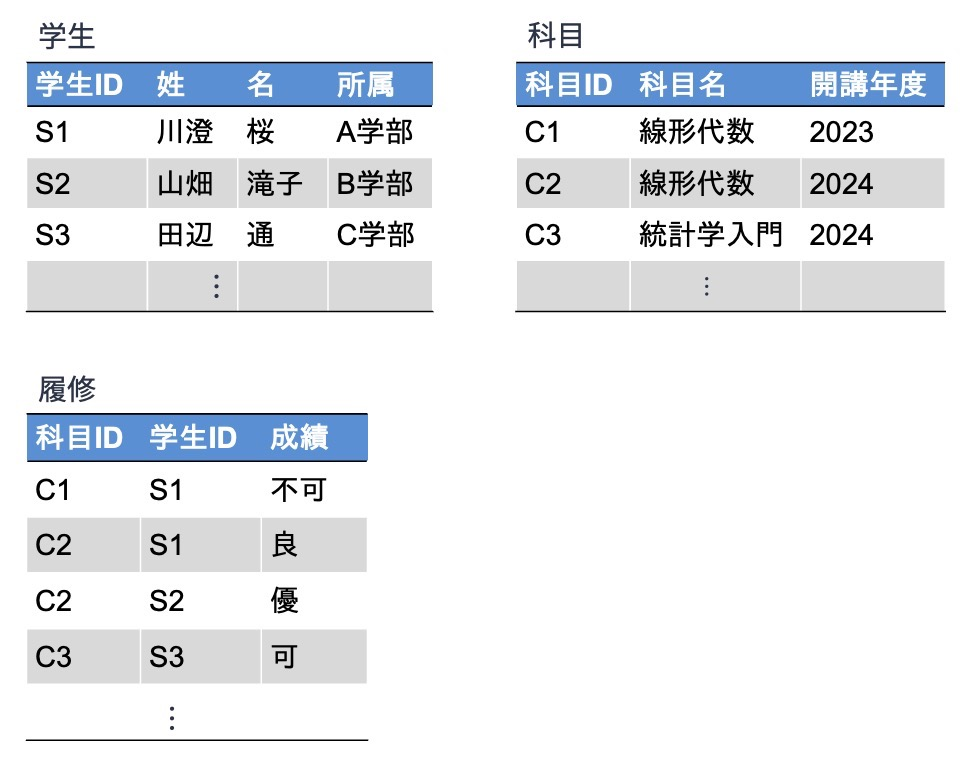
\includegraphics[width=1.0\textwidth]{figure/relational-data-model/score-db.jpg}
    \caption{成績管理データベース}
    \label{fig:score-db}
\end{figure}
図中の3つの関係（表）があれば，
\begin{itemize}
\item 関係「学生」から「学生ID」が\graybox{S1}のものを探し，
\item 関係「科目」から「科目ID」が\graybox{C1}のものを探す
\end{itemize}
ことで，関係「履修」において「学生ID」が\graybox{S1}で「科目ID」が\graybox{C1}の「成績」が\graybox{不可}だった件について，具体的にどんな学生が何の科目を落としてしまった（不可になってしまった）かを把握することができる．
このとき，関係「履修」のタプルにある「科目ID」の\graybox{C1}という値が，関係「科目」のインスタンスの属性「科目ID」に含まれていなければならない（関係「科目」の科目IDの列にその値が存在しなければならない），ということは自明であろう．
関係「履修」の中にはあるが，関係「科目」には存在していなければ，データ管理として破綻していることになる．
「学生ID」の\graybox{S1}についても同様である．

上記の例では，
\begin{itemize}
\item 関係「履修」の属性「学生ID」は関係「学生」の主キーである「学生ID」と
\item 関係「履修」の属性「科目ID」は関係「科目」の主キーである「科目ID」と
\end{itemize}

紐付いていることが分かる．
言い方を変えると，関係「履修」は属性「学生ID」および「科目ID」の値を通して，関係「学生」および「科目」の情報を参照していることになる．

このように，関係スキーマ$\boldsymbol{R_1}(..., FK, ...)$と$\boldsymbol{R_2}(\underline{PK}, ...)$が与えられ，$\boldsymbol{R_1}$におけるタプルの属性$FK$の値は必ず$\boldsymbol{R_2}$におけるいずれかのタプルの主キー$PK$の値と一致するように設計されているとき，$\boldsymbol{R_1}$の属性$FK$を$\boldsymbol{R_2}$の$PK$に対する\strong{外部キー（foreign key）} と呼ぶ．
関係スキーマ上では，関係$\boldsymbol{R_1}$の属性$FK$が関係$\boldsymbol{R_2}$の主キー$PK$に対する外部キーであることを以下のように記す．
\begin{equation}
\boldsymbol{R_1}.FK \subseteq \boldsymbol{R_2}.PK
\end{equation}

図\ref{fig:score-db}の例では，関係「履修」の属性「学生ID」および「科目ID」が外部キーとなるので，関係スキーマとして
\begin{eqnarray}
履修.学生ID \subseteq 学生.学生ID \\
履修.科目ID \subseteq 科目.科目ID
\end{eqnarray}
と記す．

前置きが長くなったが，本節のテーマである\strong{参照整合性制約（referential constraint）} とは「関係スキーマにおいて外部キーが設定されたとき，そのいかなるインスタンスも設定された外部キーの条件を満たさなければいけない」という制約である．

% ---------------------------------------
\subsection{データ従属性}
% ---------------------------------------
一貫性制約として，ドメイン制約，キー制約，参照制約を挙げてきた．
関係データモデルにはこれら以外にも，データ間に成立する制約を数学的に記述する手段がある．
これを\strong{データ従属性（data dependency）} と呼ぶ．

データ従属性としては，関数従属性，多値従属性，結合従属性など，様々なものが提案されている．
\strong{関数従属性（functional dependency）} は，データ従属性の中でも最も単純で，かつ実用的なものである．
関数従属性は，「関係$\boldsymbol{R}(..., X, ..., Y, ...)$において，属性（あるいは属性集合）$X$の値が決まると属性$Y$の値も一意に決まる」という性質である．
このことを
\begin{equation}
X \to Y
\end{equation}
と記す．

例えば，関係として
\begin{equation}
連絡先(\underline{学生ID}, 名前, 学年, 大学email, 郵便番号, 都道府県, 自宅住所)
\end{equation}
が与えられたとしよう．
一般常識から，住所が決まればそれが存在する都道府県や郵便番号もひとつに決まる．
このことから，関係「連絡先」においては
\begin{eqnarray}
自宅住所 \to 郵便番号 \\
自宅住所 \to 都道府県
\end{eqnarray}
という関数従属性が定義できる．
関数従属性はキー制約を一般化したものと捉えることができる．

データ従属性は，データの更新があったときにその影響が最小限になるように関係データベースを設計する上で，極めて重要である．
それゆえ，特に関数従属性については別章で取り上げる．


% ---------------------------------------
\hrulefill
\section*{クイズ}
% ---------------------------------------
\subsubsection{Q1. 直積}
集合$S_{lang}$，$S_{popularity}$，$S_{difficulty}$を以下のように定義する：
\begin{eqnarray}
S_{lang} = \{Python, R, C^{++}\} \\
S_{popularity} = \{人気, 不人気\} \\
S_{difficulty} = \{難, 普通, 易\}
\end{eqnarray}
このとき，直積集合$S_{lang} \times S_{popularity} \times S_{difficulty}$の要素をすべて列挙せよ．

\subsubsection{Q2. 関係}
Q1で定義した集合$S_{lang}$，$S_{popularity}$，$S_{difficulty}$上の3項関係を適当に考えよ
(※ 正解は一意に決まらないので，深く悩まずクイズに取り組むこと)．


\subsubsection{Q3. 関係スキーマ}
関係スキーマ
\begin{equation}
学生(\underline{学籍番号}, 氏名, 学部, 年齢, 出身都道府県)
\end{equation}
に従う表データの例を作成せよ．
なお，表の行数は見出し行を含めて5-6行程度でよい．


\subsubsection{Q4. ドメイン}
Q3で定義した関係スキーマ「学生」の各属性について，そのドメインを定義せよ．
\begin{equation}
Dom(学籍番号) = \{ ... \}
\end{equation}
の形式で頑張って書いてみること．

\subsubsection{Q5. ドメイン制約}
Q4で定義した関係スキーマ（ドメイン定義を含む）に対して，ドメイン制約に違反しているタプルの例を2，3個列挙せよ．


\subsubsection{Q6. 候補キー（令和4年度 ITパスポート試験 問65改題）}
関係スキーマ
\begin{equation}
従業員(従業員番号, 従業員名, 部門コード, 生年月日, 住所)
\end{equation}
において，候補キーは何か．
なお，関係「従業員」は以下のような制約条件をもつ：
\begin{itemize}
\item 各従業員は重複のない従業員番号を1つだけもつ
\item 同姓同名の従業員がいてもよい
\item 各部門は重複のない部門コードを1つだけもつ
\item 1つの部門には複数名の従業員が所属する
\item 1人の従業員が所属する部門は1つだけである
\end{itemize}


\subsubsection{Q7. 主キー}
表\ref{tab:membership-management}の「会員管理」において，想定される主キーは何か．

\begin{table}[tb]
\centering
\caption{関係「会員管理」}
\begin{tabular}{@{}lllll@{}}
会員管理 &            &             &               &               \\ \midrule
\textbf{店舗コード} & \textbf{店舗名} & \textbf{会員番号} & \textbf{会員名} & \textbf{会員種別} \\ \midrule
S01            & 星ヶ丘          & 1             & 山畑 滝子        & ゴールド          \\
S01            & 星ヶ丘          & 2             & 田辺 通         & ゴールド          \\
S02            & 八事           & 1             & 北 千種         & 学生            \\
S02            & 八事           & 2             & 川澄 桜         & プラチナ          \\
S02            & 御器所          & 1             & 川澄 桜         & 一般            \\ \bottomrule
\end{tabular}
\label{tab:membership-management}
\end{table}


\subsubsection{Q8. 参照整合性制約}
以下の関係スキーマをもつ5つの関係からなるデータベースにおいて，定義すべき参照整合性制約をあげよ．
\begin{eqnarray}
顧客(\underline{顧客ID}, 氏名, 性別) \\
店舗(\underline{店舗ID}, 店舗名, 住所) \\
商品(\underline{商品ID}, 商品名, 商品カテゴリID, 単価) \\
購買(\underline{購買ID}, 店舗ID, 顧客ID, 商品ID, 個数, 購買日) \\
商品カテゴリ(\underline{商品カテゴリID}, カテゴリ名)
\end{eqnarray}

\chapter{SQL -- その1}\label{chap:sql-part1}

\ref{chap:relational-data-model}章まで定義の話が続いてきたので，本章からは関係データベースを扱うための実践的な話題に移りましょう．

データベースからデータを抽出したり，データベースに新しいデータを登録したりするには，データベースを操作するための具体的なツールが必要となります．
\strong{SQL（Structured Query Language）} は関係データベースの操作に特化した言語です．
SQLはISOによって国際的に標準化されています．
よく用いられる関係データベース管理システム（RDBMS）としては，MySQL\footnote{\url{https://ja.wikipedia.org/wiki/MySQL}}やPostgreSQL\footnote{\url{https://ja.wikipedia.org/wiki/PostgreSQL}}，Oracle Database\footnote{\url{https://ja.wikipedia.org/wiki/Oracle_Database}}，Microsoft SQL Server\footnote{\url{https://ja.wikipedia.org/wiki/Microsoft\_SQL\_Server}}などが挙げられますが，どのRDBMSにもSQLは実装されています．

SQLを使うことで，関係データベースのユーザは
\begin{itemize}
\item データの登録（Create）
\item データの読み出し（Read）
\item データの更新（Update）
\item データの削除（Delete）
\end{itemize}
が可能となります\footnote{データの作成，読み出し，更新，削除はデータベースに求められる主要な操作で，それぞれの頭文字を取ってCRUD（クラッド）と呼ばれる．}．
ここで，関係データベースのユーザは人間だけでなく，アプリケーションなどのプログラムであっても構いません．
例えば，データ分析者は，データベースから分析に必要となるデータを抽出する際にSQLを使っています．
また，ショッピングサイトでは，消費者がある商品の注文ボタンを押すと，ウェブアプリケーションのプログラムがSQLを通じてデータベースに注文記録を登録するということが行われています．

ところで，SQLはデータベースに対する問い合わせ言語であって，プログラミング言語ではありません．
SQLはプログラミング言語に比べて覚えることは少なく，問い合わせ内容を英語に近い形で書き下すことができるよう設計されています．
もしあなたがデータ分析人材を目指しているのであれば，ソフトウェアを開発することが目的ではありませんから，高度なプログラミング能力を持つ必要はありません．
しかし，大量のデータを活かすことが期待されている今日，関係データベースに納められた大量のデータを自由自在に扱うためには，\strong{SQLの習得は必須}です．
本章ではデータ分析の基本となる「読み出し（Read）」の基礎に絞って解説し，複雑な読み出しやレコードの登録，更新などは次章以降で説明します．


\begin{notebox}{SQLの読み方}
SQLは「エス・キュー・エル」と読む．SQLは1970年代にIBM社が開発したデータベース管理システムSystem Rの操作言語SEQUELを起源としています\cite{SEQUEL}．
関係データベースに熱狂していた世代の人の中には，SEQUELの名残でSQLのことを「シークエル」と呼ぶ人もいます．
\end{notebox}

\begin{warningbox}{SQLにも方言がある}
RDBMSによって，SQLで使用できる関数が異なったりすることがあります．
特にSQLiteについては，簡易的なRDMBSということもあり，他のRDBMSでは実装されている機能や関数が実装されていない場合があります．
自分が書いたSQL文がうまく動作しない場合は，マニュアルに当たってみてください．
\end{warningbox}


\section{SQLと関係データモデルの比較}\label{chap:sql-vs-relational-data-model}
SQLは関係データベースを操作する言語で，それが扱うデータモデルは関係データモデルを実用的に拡張したものです．
ところが，「実用」のSQLデータモデルと「理論」の関係データモデルでは，同様の概念が異なる用語で定義されていることがあります．
以下，SQLと関係データモデルの用語の比較です．

\begin{table}[h]
    \centering
    \caption{SQLと関係データモデルの用語の比較}
    \begin{tabular}{ll}
    \toprule
    \textbf{関係データモデル}             & \textbf{SQL}            \\ \midrule
    関係（リレーション; relation） & 表（テーブル; table） \\
    タプル（tuple）           & レコード or 行（row） \\
    属性（attribute）        & 列（カラム; column） \\
    定義域（ドメイン; domain）    & データ型           \\ \bottomrule
    \end{tabular}
    \label{tab:sql-vs-relational-data-model}
\end{table}

表\ref{tab:sql-vs-relational-data-model}はSQLと関係データモデルで登場する類似概念を整理していますが，これら以外に重要な違いが3つあります．
1つ目が，SQLでは同じ内容を示すレコードの存在（重複）が許されることがあるという点です．
関係データモデルにおいてSQLのレコードに相当するのがタプルですが，タプルは（数学的な）集合の要素であるため，関係データモデルでは同じ内容のタプルを重複して存在することは許されていません．
ところが，SQLでは問い合わせの結果の中では同じ内容のレコードの存在が許されています．
これは，現実の関係データベースに対する問い合わせにおいては，レコードが重複することを許可しないと都合が悪い場合があるからです．
例えば，同じカテゴリに属する商品の売り上げの平均額を計算する場合，カテゴリ名に対応する商品の売り上げ高をまず抽出する必要がありますが，仮にカテゴリAに属する商品XとYの売り上げが同じ額の場合，抽出したレコードには同じ内容のレコードが2つ含まれることになります．
このとき，もしSQLが同じ内容のレコードの重複を許さなければ，商品X，Yいずれかの売り上げ情報が消えることになり，売り上げ額の平均計算が正しく行えなくなります．

違いの2つ目は，SQLでは問い合わせ結果に対して順序関係を定義できる点です．
関係データモデルでは関係中のタプルには順序関係がありません．
タプルは集合の要素であり，集合には順序の概念がないからです．
ところが，実用的な関係データベースに対する問い合わせにおいては，問い合わせ結果のレコードに順序を定義したい場合があります．
例えば，売り上げを記録している関係があったとき，売り上げ順に関係中のタプルを並べたくなりますよね．
関係データモデルのタプルと同様，SQLにおいてもテーブル中のレコードには順序関係がありません．
しかしながら，先のようなニーズに応えるため，SQLでは問い合わせの結果得られたレコードには順序づけを行うことができます．

3つ目の違いは，\strong{NULL値}の有無です．
関係データモデルでは各属性は必ずドメインで定義された値を持ちます．
一方，現実的にはある属性の値が存在しない，あるいは未定義（不明）のケースがあり得ます．
このような状況を表現するために，SQLでは特殊な値である\strong{NULL値}（ヌルと読む）を用います．

関係データモデルとSQLの対応付けが終わりましたので，早速関係データを具体的に操作する方法を見ていきましょう．


\section{準備}
以下の説明では，SQLite\footnote{\url{https://www.sqlite.org/index.html}}と解説用に作成した仮想データを用いてSQLについて解説します．

\subsection{SQLite}
SQLiteは個人用のPCでも簡単に利用できる，軽量なRDBMSです．
SQLiteは軽量であるものの，SQLの基本的な機能については十分にサポートされているため，SQLの学習に適しています．

SQLiteを利用する最も簡単な方法は，DB Browser for SQLiteを利用することです．
DB Browser for SQLiteの公式サイト（\url{https://sqlitebrowser.org/}）にはWindows，macOS，Linux向けのインストーラが配布されているので，本書で説明するSQLを実際に実行してみたい方はダウンロードしてください．

\subsection{仮想データ}
本章では，SQL解説用に著者が作成した仮想データを用います．
用意した仮想データは，こちらのURL（\url{https://github.com/trycycle/database-textbook/xxxx}）よりダウンロードできます．
ダウンロードしたファイル\graybox{sql1-example.db}はSQLiteのデータベースファイルです．
DB Browser for SQLiteなどのSQLiteクライアントソフトを用いて，本章用の関係データベースを操作することができます．

ダウンロードしたデータは，1章で取り上げたような小売店ショッピングサイトに掲載された商品の情報を管理する関係データベースです．
この関係データベースには，表\ref{table:product-table}のように，商品ID，商品名，カテゴリ，メーカー，価格，在庫数を列（属性）として持つ「商品」テーブルが格納されています．
以後，このテーブルが格納された関係データベースが手元にあると想定して，SQLの使い方を説明します．
\begin{table}[h]
    \centering
    \caption{「商品」テーブル}
    \scalebox{0.93}{
    \begin{tabular}{@{}llllll@{}}
    \toprule
    \textbf{商品ID} & \textbf{商品名} & \textbf{カテゴリ} & \textbf{メーカー} & \textbf{価格} & \textbf{在庫数} \\ \midrule
    P001 & 国産カレーパン         & パン     & A製パン       & 270 & 206 \\
    P002 & 職人仕込みクロワッサン & パン     & Bフーズ & 230 & 443 \\
    P003 & 国産チキンカレー       & レトルト & C食品     & 420 & 149 \\
    P004 & 天然中華丼の素         & レトルト & Dフード       & 180 & 166 \\
    P005 & 味わい焼肉のたれ       & 調味料   & E食品         & 890 & 18  \\
         &                        & $\vdots$ &                  &     &      \\
    P500 & 辛口めんつゆ          & 調味料 & E食品 & 590 & 19 \\ \bottomrule
    \end{tabular}
    }
    \label{tab:product-table}
\end{table}


\section{SQLの基本形}
関係データベースに対する最も典型的な問い合わせ要求は，
\begin{itemize}
\item 特定の\strong{表（table，テーブル）}から
\item \strong{列（column，カラム）} が特定の条件を満たす\strong{行（row）}\footnote{レコード（record）と呼ぶこともある．} を見つけ出し
\item 結果を表形式で出力する
\end{itemize}
というものです．
問い合わせのために記述するSQL文のことを\strong{クエリ（query）} と呼びます．

SQLによる代表的なクエリは，コード\ref{code:first-sql}に記したようなの形式の\strong{SELECT文}です．
\begin{figure}[h]
    \begin{minted}[gobble=1,
        bgcolor=background,
        fontsize=\small,
        linenos=false,
        xleftmargin=0em]{sql}

    SELECT
        商品名
    FROM
        商品
    WHERE
        在庫数 >= 100;

    \end{minted}
    \captionsetup{name=コード}
    \caption{単純なSELECT文}
    \label{code:first-sql}
\end{figure}
このクエリは，
\begin{framed}
「商品」テーブルから「在庫数」という列の値が100以上である行を見つけ，その行の列「商品名」を出力してください
\end{framed}
という問い合わせ要求を表現したものです．
これら要求を表現するために，コード\ref{code:first-sql}のクエリでは
\begin{itemize}
\item \graybox{SELECT}句を用いて「問い合わせ結果に表示したい列情報」，
\item \graybox{FROM}句を用いて「参照したい表」，
\item \graybox{WHERE}句を用いて「表示する際の条件」
\end{itemize}
を指定しています．
上記要求を英語に直してみると，SQL文は問い合わせ要求をできるだけ直感的に表現しようとしていることが見て取れます．

コード\ref{code:first-sql}のクエリは単純な例に過ぎませんが，関係データベースからデータを引っ張ってくる問い合わせについては，コード\ref{code:sql-structure}のように必ず\graybox{SELECT}句から始まるクエリが用いられます．
\begin{figure}[h]
    \begin{minted}[gobble=1,
        bgcolor=background,
        fontsize=\small,
        linenos=false,
        xleftmargin=0em]{sql}

    SELECT
        列名1, 列名2, ...
    FROM
        参照する表1, 表2, ...
    [WHERE 条件]
    [GROUP BY 列名1, 列名2, ...]
    [HAVING 条件]
    [ORDER BY 列名1, 列名2, ...]
    [LIMIT 数字];

    \end{minted}
    \captionsetup{name=コード}
    \caption{SQLの構文}
    \label{code:sql-structure}
\end{figure}
問い合わせを行うSQL文\ref{code:sql-structure}において，問い合わせ結果に表示したい情報を指定する\graybox{SELECT}句，および問い合わせの際に参照するテーブルを指定している\graybox{FROM}句は必須です．
これらが欠けていると，SQL文は動作しません．
一方，\graybox{[ ]}で囲まれた箇所については，書かなくてもSQLとして動作します．
なお，\graybox{SELECT}や\graybox{FROM}，\graybox{WHERE}，\graybox{GROUP BY}，\graybox{HAVING}，\graybox{ORDER BY}，\graybox{LIMIT}といった句の意味については後ほど説明しますが，どの句も\strong{この順序で使う}必要があります．
例えば，\graybox{HAVING}句は必ず\graybox{GROUP BY}句の後ろに書きます．
また，クエリの末尾にはセミコロン（;）をつけ忘れてはいけません．
文法に違反するSQL文は動作しないので，注意しましょう．


\section{射影（SELECT） -- 列の抽出}
最も単純なSQLは\graybox{SELECT}句と\graybox{FROM}句のみを使うものです．
\strong{射影（projection）}は，\graybox{FROM}句で指定されたテーブルから\graybox{SELECT}句で指定した特定の列のデータのみを抽出する操作です．

例題として用いる「商品」テーブルには，列として「商品ID」「商品名」「カテゴリ」「メーカー」「価格」「在庫数」がありますが，用途によっては特定の列のデータのみ欲しい場合があります．
そのようなケースで用いるのが射影です．
例えば，「商品」テーブルから「商品名」「メーカー」「価格」の列のデータのみを抽出する場合，SQL文はコード\ref{code:sql-select}となります．
\begin{figure}[h]
    \begin{minted}[gobble=1,
        bgcolor=background,
        fontsize=\small,
        linenos=false,
        xleftmargin=0em]{sql}

    SELECT
        商品名, メーカー, 価格
    FROM
        商品;

    \end{minted}
    \captionsetup{name=コード}
    \caption{射影 - SELECT}
    \label{code:sql-select}
\end{figure}
このSQL文を実行すると，表\ref{tb:sql-select}のように，\graybox{SELECT}句内で指定した「商品名」「メーカー」「価格」列のデータのみが抽出されます．

\begin{table}[h]
    \centering
    \caption{「商品」テーブルに対する射影の結果}
    \begin{tabular}{@{}lll@{}}
    \toprule
    \textbf{商品名} & \textbf{メーカー} & \textbf{価格} \\ \midrule
    国産カレーパン & A製パン & 270 \\
    職人仕込みクロワッサン & Bフーズ & 230 \\
    国産チキンカレー & C食品 & 420 \\
    天然中華丼の素 & Dフード & 180 \\
    味わい焼肉のたれ & E食品 & 890 \\
    &   $\vdots$      &      \\
    辛口めんつゆ & E食品 & 590  \\ \bottomrule
    \end{tabular}
    \label{tb:sql-select}
\end{table}

「商品」テーブルは合計で500行のレコードが格納されているため，表が縦に長くなり，PCの画面からはみ出してしまいます．
SQL文の問い合わせで得られた結果のうち，先頭の$N$行だけを表示させたい時は，コード\ref{code:sql-select2}のようにLIMIT句を使うとよいでしょう．
コード\ref{code:sql-select2}を実行すると，表\ref{tb:sql-select2}のように，先頭の5行だけが表示されます．
\begin{figure}[h]
    \begin{minted}[gobble=1,
        bgcolor=background,
        fontsize=\small,
        linenos=false,
        xleftmargin=0em]{sql}

    SELECT
        商品名, メーカー, 価格
    FROM
        商品;
    LIMIT 5;  --- コメント:先頭の5件のみ表示

    \end{minted}
    \captionsetup{name=コード}
    \caption{「商品」テーブルに対して射影を行い，その結果の先頭5件だけ表示するSQL文}
    \label{code:sql-select2}
\end{figure}
\begin{table}[h]
    \centering
    \centering
    \caption{「商品」テーブルに対する射影の結果（先頭5件に限定）}
    \begin{tabular}{@{}lll@{}}
    \toprule
    \textbf{商品名} & \textbf{メーカー} & \textbf{価格} \\ \midrule
    国産カレーパン & A製パン & 270 \\
    職人仕込みクロワッサン & Bフーズ & 230 \\
    国産チキンカレー & C食品 & 420 \\
    天然中華丼の素 & Dフード & 180 \\
    味わい焼肉のたれ & E食品 & 890 \\ \bottomrule
    \end{tabular}
    \label{tb:sql-select2}
\end{table}

コード\ref{code:sql-select2}のSQL文では，表示する列を「商品名」「メーカー」「価格」に限定していました．
一方で，テーブルがもつすべての列情報を表示させたい場合もあるでしょう．
真面目にやるならば\graybox{SELECT}句にすべての列名を列挙することになりますが，テーブルが持つ列の数が多い場合は大変です．
このような場合，コード\ref{code:sql-select3}のように\graybox{SELECT}句に\strong{アスタリスク（*）}を使えばよいです\footnote{計算機科学の世界では，アスタリスク（*）は「なんでもあり（すべて）」を表す「ワイルドカード」と呼ばれる記号としてよく使われます．}．
アスタリスクを用いると，表\ref{tb:sql-select3}のようにすべての列名を列挙するのと同等の結果が得られます．
\begin{figure}[h]
    \begin{minted}[gobble=1,
        bgcolor=background,
        fontsize=\small,
        linenos=false,
        xleftmargin=0em]{sql}

    SELECT
        *
    FROM
        商品
    LIMIT 5;

    \end{minted}
    \captionsetup{name=コード}
    \caption{アスタリスクを用いてすべての列を列挙するSQL文}
    \label{code:sql-select3}
\end{figure}

\begin{table}[h]
    \centering
    \caption{「商品」テーブルに対する射影の結果（すべての列について，先頭の5件のレコードを表示）}
    \scalebox{0.93}{
    \begin{tabular}{@{}llllll@{}}
    \toprule
    \textbf{商品ID} & \textbf{商品名} & \textbf{カテゴリ} & \textbf{メーカー} & \textbf{価格} & \textbf{在庫数} \\ \midrule
    P001 & 国産カレーパン & パン & A製パン & 270 & 206 \\
    P002 & 職人仕込みクロワッサン & パン & Bフーズ & 230 & 443 \\
    P003 & 国産チキンカレー & レトルト & C食品 & 420 & 149 \\
    P004 & 天然中華丼の素 & レトルト & Dフード & 180 & 166 \\
    P005 & 味わい焼肉のたれ & 調味料 & E食品 & 890 & 18  \\ \bottomrule
    \end{tabular}
    }
    \label{tb:sql-select3}
\end{table}


\begin{tipbox}{読みやすいSQL}
SQL文では改行や余分な空白は無視されます．
例えば，コード\ref{code:sql-select3}のSQL文は\graybox{SELECT * FROM 商品 LIMIT 5;}と解釈されます．

それでも本書でわざわざ改行や余分な空白を入れてSQL文を書いているのは，SQL文を読みやすくするためです．
複雑な問い合わせを行う場合，SQL文も複雑かつ長くなります．
そういったSQL文を読むのは苦痛ですし，ミスも見落としやすくなります．
できる限りSQL文は読みやすくしておくのが良いです．
\end{tipbox}


\section{選択（WHERE） -- 行の絞り込み}
\strong{選択}とは，関係データベースから特定の条件を満たすレコードを抽出する操作です．
選択を行うには\graybox{WHERE}句を用います．
\graybox{WHERE}句を使うことで，\graybox{FROM}句で参照したテーブル中のレコードについて列の値と定数，あるいは列同士の値を比較して，条件に合致するレコードを絞り込むことができます．

\graybox{WHERE}句で使える代表的な比較演算子は，以下の通りです：
\begin{itemize}
\item $=$（等しい）
\item $!=$（等しくない）
\item $<$（より小さい）
\item $>$（より大きい）
\item $<=$（以下）
\item $>=$（以上）
\end{itemize}
例えば，「商品」テーブルから「価格」が500以上のレコードを抽出するSQL文はコード\ref{code:sql-where}のようになります．
このSQL文を実行すると，表\ref{tab:sql-where}のように，「価格」列の値が500以上のレコードのみが抽出されます．
\begin{figure}[h]
    \begin{minted}[gobble=1,
        bgcolor=background,
        fontsize=\small,
        linenos=false,
        xleftmargin=0em]{sql}

    SELECT
        *
    FROM
        商品
    WHERE
        価格 >= 500;

    \end{minted}
    \captionsetup{name=コード}
    \caption{「商品」テーブルから価格が500以上のレコードを抽出するSQL文}
    \label{code:sql-where}
\end{figure}
\begin{table}[h]
    \centering
    \caption{「商品」テーブルから価格が500以上のレコードを抽出した結果}
    \scalebox{0.93}{
    \begin{tabular}{@{}llllll@{}}
    \toprule
    \textbf{商品ID} & \textbf{商品名} & \textbf{カテゴリ} & \textbf{メーカー} & \textbf{価格} & \textbf{在庫数} \\ \midrule
    P005 & 味わい焼肉のたれ & 調味料 & E食品 & 890 & 18 \\
    P011 & 無添加麻婆豆腐の素 & レトルト & Fファーム & 520 & 299 \\
    P015 & 濃厚ごまドレッシング & 調味料 & Fファーム & 650 & 57 \\
    P019 & 贅沢焼肉のたれ & 調味料 & E食品 & 890 & 391 \\
    P021 & 味わい中華丼の素 & レトルト & C食品 & 550 & 254 \\
    &        &       $\vdots$    &     &        &       \\
    P500 & 辛口めんつゆ & 調味料 & E食品 & 590 & 19 \\ \bottomrule
    \end{tabular}
    }
    \label{tab:sql-where}
\end{table}

比較したい列のデータ型が文字列の場合は，比較したい文字列を\strong{シングルクォーテーション（'）}で囲って指定します．
コード\ref{code:sql-where2}は，「商品」テーブルから「メーカー」が「Fファーム」のレコードを抽出するSQL文の例です．
このSQL文を実行すると，表\ref{tab:sql-where2}のように，「メーカー」列の値が「Fファーム」のレコードのみが抽出されます．
\begin{figure}[h]
    \begin{minted}[gobble=1,
        bgcolor=background,
        fontsize=\small,
        linenos=false,
        xleftmargin=0em]{sql}

    SELECT
        *
    FROM
        商品
    WHERE
        メーカー = 'Fファーム';

    \end{minted}
    \captionsetup{name=コード}
    \caption{「商品」テーブルからメーカーが「恵みファーム」のレコードを抽出するSQL文}
    \label{code:sql-where2}
\end{figure}
\begin{table}[h]
    \centering
    \caption{「商品」テーブルからメーカーが「Fファーム」のレコードを抽出した結果}
    \scalebox{0.93}{
    \begin{tabular}{@{}llllll@{}}
    \toprule
    \textbf{商品ID} & \textbf{商品名} & \textbf{カテゴリ} & \textbf{メーカー} & \textbf{価格} & \textbf{在庫数} \\ \midrule
    P011 & 無添加麻婆豆腐の素 & レトルト & Fファーム & 520 & 299 \\
    P012 & じっくり煮込んだブラックコーヒー & 飲料 & Fファーム & 160 & 3 \\
    P015 & 濃厚ごまドレッシング & 調味料 & Fファーム & 650 & 57 \\
    P024 & 朝のオレンジジュース & 飲料 & Fファーム & 230 & 246 \\
    P025 & こだわりアップルジュース & 飲料 & Fファーム & 170 & 11 \\
    &               & $\vdots$     &   &        &       \\
    P491 & 無添加ビーフカレー & レトルト & Fファーム & 350 & 175 \\ \bottomrule
    \end{tabular}
    }
    \label{tab:sql-where2}
\end{table}

文字列の条件指定においては，列データに特定の文字列を含むレコードを抽出したいケースもあります．
そのようなケースではLIKE句を用います．
以下の例のように，\graybox{WHERE}句内に\graybox{LIKE \%部分文字列\%}といった文を書くと，指定した部分文字列を列データに含むレコードに絞り込むことができます．
なお，\%（パーセント）は0文字以上の任意の文字列を意味します．
以下は，「商品」テーブルから「商品名に「チョコ」の文字を含むレコードのみを抽出するSQL文の例です．
このSQL文を実行すると，表\ref{tab:sql-where3}のようなレコードが抽出されます．
\begin{figure}[h]
    \begin{minted}[gobble=1,
        bgcolor=background,
        fontsize=\small,
        linenos=false]{sql}

    SELECT
        *
    FROM
        商品
    WHERE
        商品名 LIKE '%チョコ%';

    \end{minted}
    \captionsetup{name=コード}
    \caption{「商品」テーブルから商品名に「チョコ」を含むレコードを抽出するSQL文}
    \label{code:sql-where3}
\end{figure}
\begin{table}[h]
    \centering
    \caption{「商品」テーブルから商品名に「チョコ」を含むレコードを抽出した結果}
    \scalebox{0.93}{
    \begin{tabular}{@{}llllll@{}}
    \toprule
    \textbf{商品ID} & \textbf{商品名} & \textbf{カテゴリ} & \textbf{メーカー} & \textbf{価格} & \textbf{在庫数} \\ \midrule
    P028 & 昔ながらのミルクチョコレート & 菓子 & C食品 & 220 & 458 \\
    P030 & 国産ミルクチョコレート & 菓子 & I製菓 & 310 & 117 \\
    P038 & 贅沢チョココロネ & パン & A製パン & 210 & 354 \\
    P041 & 天然チョココロネ & パン & Oベーカリー & 390 & 81 \\
    P070 & こだわりミルクチョコレート & 菓子 & N製菓 & 400 & 364 \\
    &               & $\vdots$     &   &        &       \\
    P493 & さくさくチョココロネ & パン & Bフーズ & 210 & 340 \\ \bottomrule
    \end{tabular}
    }
    \label{tab:sql-where3}
\end{table}
「チョコ」の前後にパーセント記号をつけることによって，商品名のどこかに「チョコ」という文字列が現れるレコードを絞り込んでいます．
もし\graybox{LIKE}句の条件を\graybox{\%チョコ\%}ではなく\graybox{\%チョコ}にした場合，「無添加 チョコチップパン」のように文末がチョコで終わらない商品名のレコードはマッチしなくなります．

\begin{notebox}{SQLの処理順序}
    \graybox{SELECT}文による問い合わせが行われたとき，関係データベース管理システムは以下のステップで処理を行います．
    \begin{enumerate}
    \item FROM句で指定した表を参照
    \item 表中の各レコードがWHERE句で指定された条件を満たしているかを確認
    \item ステップ2で条件を満たしていると判定された行のみ，その行にあるSELECT句で指定した列のデータを表示
    \end{enumerate}
\end{notebox}

\graybox{WHERE}句では条件を複数指定することもできます．
複数条件は，条件を論理演算子である\graybox{AND}もしくは\graybox{OR}で結合して表現します．
この際，
\begin{itemize}
\item \graybox{条件1 AND 条件2}と指定すれば，条件1と条件2をともに満たすレコード
\item \graybox{条件1 OR 条件2}と指定すれば，条件1もしくは条件2のいずれかを満たすレコード
\end{itemize}
を抽出することができます．

コード\ref{code:sql-where4}は，「商品」テーブルからメーカーが「N製菓」でかつ価格が500以上のレコードを抽出するSQL文の例です．
このSQLを実行すると，表\ref{tab:sql-where4}のように，「メーカー」列の値が「N製菓」でかつ「価格」列の値が500以上のレコードが抽出され，その「商品名」「価格」「在庫数」の値が表示されます．
\begin{figure}[h]
    \begin{minted}[gobble=1,
        bgcolor=background,
        fontsize=\small,
        linenos=false]{sql}

    SELECT
        商品名, 価格, 在庫数
    FROM
        商品
    WHERE
        (メーカー = 'N製菓')
        AND (価格 >= 500);

    \end{minted}
    \captionsetup{name=コード}
    \caption{「商品」テーブルから「メーカー」が「N製菓」でかつ「価格」が500以上のレコードを抽出するSQL文（表示する列は「商品名」「価格」「在庫数」限定）}
    \label{code:sql-where4}
\end{figure}
\begin{table}[h]
    \centering
    \caption{「商品」テーブルから「メーカー」が「N製菓」でかつ「価格」が500以上のレコードを抽出し，「商品名」「価格」「在庫数」の値を表示した結果}
    \scalebox{1.00}{
    \begin{tabular}{@{}lll@{}}
    \toprule
    \textbf{商品名} &  \textbf{価格} & \textbf{在庫数} \\ \midrule
職人仕込み塩クラッカー & 540 & 322 \\
贅沢ビスケット & 500 & 163 \\
特製塩クラッカー & 510 & 273 \\ \bottomrule
    \end{tabular}
    }
    \label{tab:sql-where4}
\end{table}

\begin{tipbox}{条件の明確化}
    条件の前後に丸括弧をつけることで，条件の記述範囲を明確にすることができます．
    条件の範囲やAND/ORのかかる順序をわかりやすくするためにも，条件が複雑な場合は条件の前後に丸括弧をつけることをオススメします．
\end{tipbox}

\section{重複の除外}
\ref{chap:sql-vs-relational-data-model}節で述べたように，SQLはレコードの重複を許しています．
そのため，SQL文の実行結果には重複するレコードが含まれることがあります．

例えば，「商品」テーブルの「メーカー」列に着目して，「商品」テーブルで取り扱っている商品のメーカーの一覧を抽出することを考えてみましょう．
これまで説明してきた内容を踏まえると，コード\ref{code:sql-undistinct}のように「メーカー」列を射影するSQL文でメーカーの一覧を抽出できると考えた方がいるかもしれません．
\begin{figure}[h]
    \begin{minted}[gobble=1,
        bgcolor=background,
        fontsize=\small,
        linenos=false]{sql}

    SELECT
        メーカー
    FROM
        商品;

    \end{minted}
    \captionsetup{name=コード}
    \caption{「商品」テーブルから「メーカー」列の値を抽出するSQL文}
    \label{code:sql-undistinct}
\end{figure}
ところが，期待に反してコード\ref{code:sql-undistinct}のSQL文を実行すると，表\ref{tab:sql-undistinct}のように「メーカー」列の値が重複しているレコードが抽出されてしまいます．
\begin{table}[h]
    \centering
    \caption{「商品」テーブルから「メーカー」列の値を抽出した結果}
    \scalebox{1.00}{
    \begin{tabular}{@{}l@{}}
    \toprule
    \textbf{メーカー} \\ \midrule
A製パン \\
Bフーズ \\
C食品 \\
Dフード \\
E食品 \\
$\vdots$ \\
E食品 \\
\bottomrule
    \end{tabular}
    }
    \label{tab:sql-undistinct}
\end{table}

レコードの重複を除いた結果を出力したい場合は，\graybox{SELECT}の直後に\graybox{DISTINCT}を指定します．
コード\ref{code:sql-undistinct}はコード\ref{code:sql-distinct}のように書き換えることで，重複を除いたレコード，つまり「商品」テーブルにある商品を取り扱っているメーカーの一覧を抽出することができます（結果は\ref{tab:sql-distinct}）．
\begin{figure}[h]
    \begin{minted}[gobble=1,
        bgcolor=background,
        fontsize=\small,
        linenos=false]{sql}

    SELECT DISTINCT
        メーカー
    FROM
        商品;

    \end{minted}
    \captionsetup{name=コード}
    \caption{「商品」テーブルから「メーカー」列の値を重複を省いて抽出するSQL文}
    \label{code:sql-distinct}
\end{figure}
\begin{table}[h]
    \centering
    \caption{「商品」テーブルから「メーカー」列の値を重複を省いて抽出した結果}
    \scalebox{1.00}{
    \begin{tabular}{@{}l@{}}
    \toprule
    \textbf{メーカー} \\ \midrule
A製パン \\
Bフーズ \\
C食品 \\
Dフード \\
E食品 \\
$\vdots$ \\
Q醤油 \\ \bottomrule
    \end{tabular}
    }
    \label{tab:sql-distinct}
\end{table}



\section{整列（ORDER BY）}
データ分析では，大きいもの（小さいもの）順にデータを\strong{整列（ソート）}させたいケースが多々あります．
そのようなケースで使用するのが\graybox{ORDER BY}句です．

SQLでは，コード\ref{code:sql-orderby}のように\graybox{ORDER BY}の後に列名を指定することで，抽出したレコードを指定した列の値の小さいもの順（昇順） に並び替えることができます．
このSQL文を実行すると，表\ref{tab:sql-orderby}のように，「商品」テーブルから在庫数の少ない順にレコードが抽出されます．
\begin{figure}[h]
    \begin{minted}[gobble=1,
        bgcolor=background,
        fontsize=\small,
        linenos=false]{sql}

    SELECT
        *
    FROM
        商品
    ORDER BY
        在庫数
    LIMIT 5; --- 先頭の5件のみ表示

    \end{minted}
    \captionsetup{name=コード}
    \caption{「商品」テーブルから在庫数の少ない順にレコードを上位5件抽出するSQL文}
    \label{code:sql-orderby}
\end{figure}
\begin{table}[h]
    \centering
    \caption{「商品」テーブルから在庫数の少ない順にレコードを抽出した結果（上位5件）}
    \scalebox{0.93}{
    \begin{tabular}{@{}llllll@{}}
    \toprule
    \textbf{商品ID} & \textbf{商品名} & \textbf{カテゴリ} & \textbf{メーカー} & \textbf{価格} & \textbf{在庫数} \\ \midrule
P074 & 贅沢カレーパン & パン & Oベーカリー & 460 & 2 \\
P084 & 天然親子丼の素 & レトルト & Mフーズ & 470 & 2 \\
P012 & じっくり煮込んだブラックコーヒー & 飲料 & Fファーム & 160 & 3 \\
P125 & 甘口パスタソース & レトルト & Fファーム & 460 & 3 \\
P157 & 辛口シチュー & レトルト & Dフード & 620 & 3 \\
 \bottomrule
    \end{tabular}
    }
    \label{tab:sql-orderby}
\end{table}

\graybox{ORDER BY}はデフォルト設定では指定した列の値が小さいもの順（昇順，in ascending order）にレコードをソートします．
大きいもの順（降順, in descending order）でソートしたい場合は，\graybox{ORDER BY}で列名を指定する際，列名の後に\graybox{DESC}キーワードを付けます．
コード\ref{code:sql-orderby2}は，「商品」テーブルから在庫数が多いもの順にレコードを抽出するSQL文の例です．
このSQL文の実行結果は，表\ref{tab:sql-orderby2}のようになります．
\begin{figure}[h]
    \begin{minted}[gobble=1,
        bgcolor=background,
        fontsize=\small,
        linenos=false]{sql}

    SELECT
        *
    FROM
        商品
    ORDER BY
        在庫数 DESC
    LIMIT 5; --- 先頭の5件のみ表示

    \end{minted}
    \captionsetup{name=コード}
    \caption{「商品」テーブルから在庫数の多い順にレコードを上位5件抽出するSQL文}
    \label{code:sql-orderby2}
\end{figure}
\begin{table}[h]
    \centering
    \caption{「商品」テーブルから在庫数の多い順にレコードを抽出した結果（上位5件）}
    \scalebox{0.93}{
    \begin{tabular}{@{}llllll@{}}
    \toprule
    \textbf{商品ID} & \textbf{商品名} & \textbf{カテゴリ} & \textbf{メーカー} & \textbf{価格} & \textbf{在庫数} \\ \midrule
P089 & カロリーオフビスケット & 菓子 & K製菓 & 270 & 500 \\
P179 & 国産ポテトチップス & 菓子 & C食品 & 190 & 500 \\
P370 & プレミアムハンバーグ & レトルト & Dフード & 590 & 498 \\
P364 & プレミアムミートボール & レトルト & Fファーム & 960 & 496 \\
P422 & 天然のど飴 & 菓子 & I製菓 & 130 & 496 \\
 \bottomrule
    \end{tabular}
    }
    \label{tab:sql-orderby2}
\end{table}


\section{集約関数}
合計値や平均値の計算などのデータの集計は，データ集合の特徴を知る上での基礎となります．
関係データベースから抽出したレコード集合に対して集計処理を行いたい場合は，\strong{集約関数（aggregate functions）}を用います．

SQLに実装されている代表的な集約関数は以下の通りです：
\begin{itemize}
\item \graybox{SUM}: 合計値の計算
\item \graybox{MAX}: 最大値の計算
\item \graybox{MIN}: 最小値の計算
\item \graybox{AVG}: 平均値の計算
\item \graybox{COUNT}: 行数のカウント
\end{itemize}
各種関数の引数には計算に用いたい列名などを指定します．
（次節で解説する\graybox{GROUP BY}句を用いない場合）集約関数は，\strong{\graybox{WHERE}句までで絞り込まれたレコード全体を1つのグループと見なして}集計処理を行います．

例えば，「商品」テーブルから「メーカー」がL食品のレコードだけに限定して，商品の「在庫数」の合計値を計算することを考えましょう．
合計値を求める集約関数は\graybox{SUM}です．
コード\ref{code:sql-sum}のように\graybox{SUM}関数の引数に「在庫数」を指定することで，「在庫数」の合計値を計算できます（結果は\ref{tab:sql-sum}）．
\begin{figure}[h]
    \begin{minted}[gobble=1,
        bgcolor=background,
        fontsize=\small,
        linenos=false]{sql}

    SELECT
        SUM(在庫数)
    FROM
        商品
    WHERE
        メーカー = 'L食品';

    \end{minted}
    \captionsetup{name=コード}
    \caption{「商品」テーブルから「メーカー」がL食品のレコードに限定して「在庫数」の合計値を計算するSQL文}
    \label{code:sql-sum}
\end{figure}
\begin{table}[h]
    \centering
    \caption{「商品」テーブルから「メーカー」がL食品のレコードに限定して「在庫数」の合計値を計算した結果}
    \scalebox{0.93}{
    \begin{tabular}{@{}r@{}}
    \toprule
    \textbf{SUM(在庫数)} \\ \midrule
8641 \\
 \bottomrule
    \end{tabular}
    }
    \label{tab:sql-sum}
\end{table}

\graybox{SELECT}句に複数の集約関数を指定することで，複数の集計処理を同時に行うこともできます．
コード\ref{code:sql-multiple-aggregates}は，「商品」テーブルから「メーカー」がL食品のレコードだけに限定して，商品の「在庫数」の合計値，平均値，最大値と最小値の差を同時に計算するSQL文の例です（結果は表\ref{tab:sql-multiple-aggregates}）．
\begin{figure}[h]
    \begin{minted}[gobble=1,
        bgcolor=background,
        fontsize=\small,
        linenos=false]{sql}

    SELECT
        SUM(在庫数),
        AVG(在庫数),
        MAX(在庫数) - MIN(在庫数)
    FROM
        商品
    WHERE
        メーカー = 'L食品';

    \end{minted}
    \captionsetup{name=コード}
    \caption{「商品」テーブルから「メーカー」がL食品のレコードに限定して，「在庫数」の合計値，平均値，最大値と最小値の差を同時に計算するSQL文}
    \label{code:sql-multiple-aggregates}
\end{figure}
\begin{table}[h]
    \centering
    \caption{「商品」テーブルから「メーカー」がL食品のレコードに限定して「在庫数」の合計値，平均値，最大値と最小値の差を同時に計算した結果}
    \scalebox{0.93}{
    \begin{tabular}{@{}rrr@{}}
    \toprule
    \textbf{SUM(在庫数)} & \textbf{AVG(在庫数)} & \textbf{MAX(在庫数) - MIN(在庫数)} \\ \midrule
8641 & 246.9 & 477 \\
 \bottomrule
    \end{tabular}
    }
    \label{tab:sql-multiple-aggregates}
\end{table}

\begin{notebox}{集約関数におけるNULL値の扱い}
\graybox{SUM}や\graybox{AVG}といった集約関数は，NULL値を無視して計算を行います．
例えば，\graybox{AVG}関数を使って平均値を計算する際，分母の件数にはNULL値を含むレコードはカウントされないので注意しましょう．
\end{notebox}

\begin{notebox}{様々な演算子}
\graybox{SELECT}句や\graybox{WHERE}句の中では，四則演算も行うことができます．
加算（+），減算（-），乗算（*），除算（/）といった四則演算のための演算子以外にも，余りを求めるための剰余演算子（\%），絶対値を求めるABS関数といった様々な算術演算ツールが用意されています．
気になった演算があればマニュアルを調べてみてください．
\end{notebox}

\graybox{COUNT}関数は行数（レコード数）をカウントすることができます．
\graybox{COUNT}関数の引数には，すべての列を意味するアスタリスク（*）が用いられることが多いです．
コード\ref{code:sql-count}は，「商品」テーブルに格納されたレコード数を調べるSQL文です（結果は表\ref{tab:sql-count}）．
このSQL文は\graybox{SELECT * FROM 商品;}の実行結果の行数を数えていると考えればOKです．
\begin{figure}[h]
    \begin{minted}[gobble=1,
        bgcolor=background,
        fontsize=\small,
        linenos=false]{sql}

    SELECT
        COUNT(*)
    FROM
        商品;

    \end{minted}
    \captionsetup{name=コード}
    \caption{「商品」テーブルに格納されたレコード数を調べるSQL文}
    \label{code:sql-count}
\end{figure}
\begin{table}[h]
    \centering
    \caption{「商品」テーブルに格納されたレコード数を調べた結果}
    \scalebox{0.93}{
    \begin{tabular}{@{}r@{}}
    \toprule
    \textbf{COUNT(*)} \\ \midrule
500 \\
 \bottomrule
    \end{tabular}
    }
    \label{tab:sql-count}
\end{table}

一方，コード\ref{code:sql-count2}のSQL文は結果だけ見るとコード\ref{code:sql-count}のSQL文と同じになりますが，振る舞いは少し異なります．
\graybox{COUNT}(列名) は，指定した列の値が「\graybox{NULL}（空値）ではないレコード」の件数を数え上げます．
要するに，\graybox{SELECT メーカー FROM 商品 WHERE メーカー IS NOT NULL;}\footnote{SQLではNULL値は特別な値なので，ある列の値がNULLであるかの判定には\graybox{IS NULL}や\graybox{IS NOT NULL}を使用します．\graybox{列名 = NULL}や\graybox{列名 != NULL}とは書きません．}の実行結果の行数を数えており，\graybox{SELECT COUNT(*) FROM 商品;}とは微妙に振るまいが異なることに注意してください．
\begin{figure}[h]
    \begin{minted}[gobble=1,
        bgcolor=background,
        fontsize=\small,
        linenos=false]{sql}

    SELECT
        COUNT(メーカー)
    FROM
        商品;

    \end{minted}
    \captionsetup{name=コード}
    \caption{「商品」テーブルに格納されたレコード数を調べるSQL文 - その2}
    \label{code:sql-count2}
\end{figure}
なお，コード\ref{code:sql-count2}の\graybox{COUNT(メーカー)}は，同じメーカー名が複数回登場した場合，それらも重複してカウントしてしまいます．
「商品」テーブルに現れるメーカーの種類数を数えたい場合は，コード\ref{code:sql-distinct-count}のSQL文のように重複を除いて数え上げたい列名の前に\graybox{DISTINCT}を付けましょう（結果は表\ref{tab:sql-distinct-count}）．
\begin{figure}[h]
    \begin{minted}[gobble=1,
        bgcolor=background,
        fontsize=\small,
        linenos=false]{sql}

    SELECT
        COUNT(DISTINCT メーカー)
    FROM
        商品;

    \end{minted}
    \captionsetup{name=コード}
    \caption{「商品」テーブルに格納された商品のメーカー数を重複を除いて調べるSQL文}
    \label{code:sql-distinct-count}
\end{figure}
\begin{table}[h]
    \centering
    \caption{「商品」テーブルに格納された商品のメーカー数を重複を除いて調べた結果}
    \scalebox{0.93}{
    \begin{tabular}{@{}r@{}}
    \toprule
    \textbf{COUNT(DISTINCT メーカー)} \\ \midrule
17 \\
 \bottomrule
    \end{tabular}
    }
    \label{tab:sql-distinct-count}
\end{table}

\begin{tipbox}{AS修飾句}
長いテーブル名，紛らわしいテーブル名，列名は混乱の元です．
SQL文やその実行結果を分かりやすくするために，SQLにはテーブル名や列名に別名を与えることができる\graybox{AS}修飾句が用意されています．
\graybox{AS}修飾句を用いて別名を与えると，別名でテーブルや列を参照することができます．
また，SQL文の実行結果の列名も付与した別名になります．

例えば，コード\ref{code:sql-distinct}は，\graybox{SELECT COUNT(DISTINCT メーカー) AS メーカー数 FROM 商品;}とすることで，実行結果の列名を「メーカー数」に変更できます．
元のSQL文の場合，列名は「COUNT(DISTINCT メーカー)」だったので，別名を付けた方がスッキリしますし分かりやすくもなります．
\end{tipbox}


\section{グループ化による集約演算（GROUP BY）}
前節までに解説した集約のためのSQL文は，\graybox{WHERE}句で絞り込まれたレコード全体に対して集計操作を行うものでした．
しかし実際にデータ分析を行う場合，レコード全体での集計にとどまらず，ある基準でレコードをまとめ，グループごとに集計を行うことも少なくありません．

\graybox{GROUP BY}句は，グループごとに集約演算を行うための機能です．
「\graybox{GROUP BY}句 + 列名」の形式で指定をすると，指定された列名について同じ値をもつレコードが1つのグループにまとめられた\strong{グループ表}が（ユーザには見えない形で）一時的に作成されます．
例えば，「商品」テーブルに対して問い合わせを行うSQL文内で「\graybox{GROUP BY} メーカー」と書くと，図\ref{fig:groupby}のようなイメージのグループ表が一時的に作成されます（点線がグループを表す）．
その後，まとめられたグループのそれぞれに対して\graybox{SELECT}句で指定された集約関数が適用されます．
\begin{figure}[h]
    \centering
    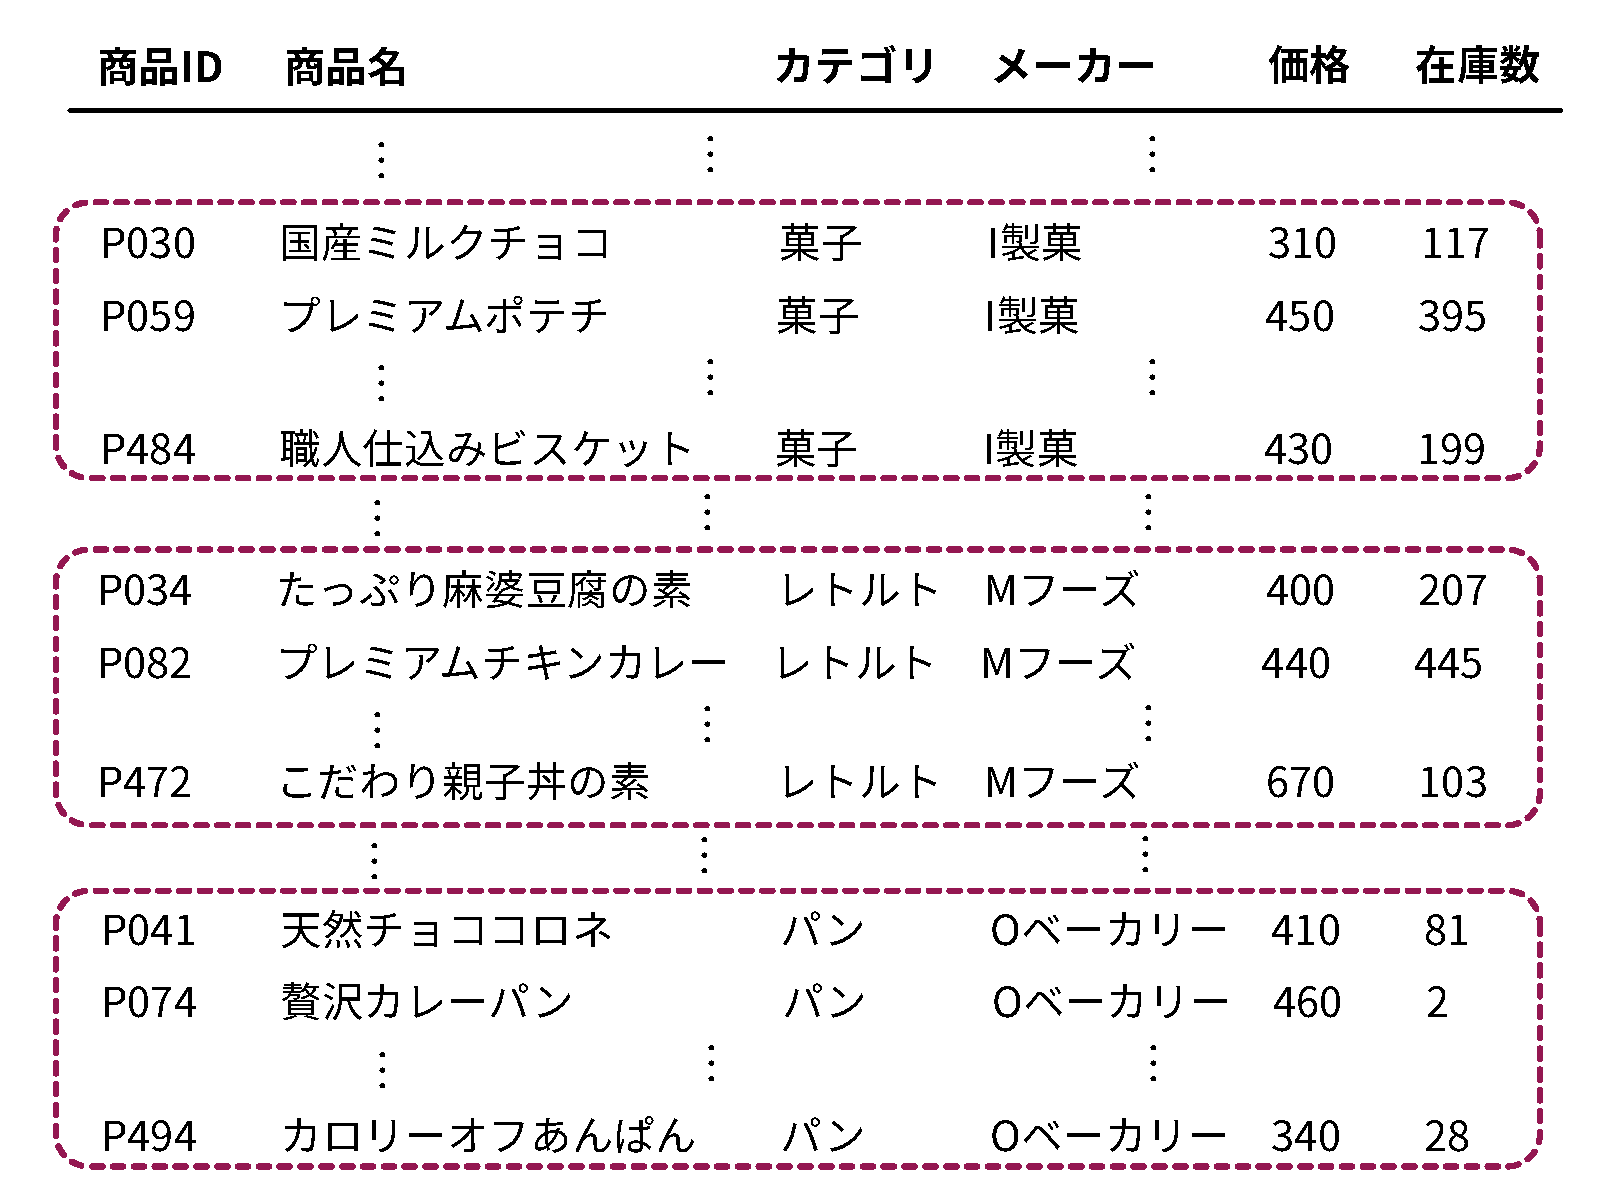
\includegraphics[width=0.95\textwidth]{figure/sql-part1/groupby.pdf}
    \caption{GROUP BY句によって「商品」テーブルを「メーカー」列の値でグループ化したイメージ図}
    \label{fig:groupby}
\end{figure}

コード\ref{code:sql-groupby}は，「商品」テーブルを用いて，「メーカー」ごとに商品の「在庫数」の平均値を計算するSQL文です．
このSQL文を実行すると，表\ref{tab:sql-groupby}のように，「商品」テーブルのレコードが「メーカー」列の値でグループ化され，グループごとに「在庫数」の平均値が計算されて表示されます．
メーカー名を表示させるために，\graybox{SELECT}句に「メーカー」列を指定していることに注意してください．
\begin{figure}[h]
    \begin{minted}[gobble=1,
        bgcolor=background,
        fontsize=\small,
        linenos=false]{sql}

    SELECT
        メーカー,
        AVG(在庫数) AS 平均在庫数 --- コメント: 列名を「平均在庫数」に変更
    FROM
        商品
    GROUP BY
        メーカー;

    \end{minted}
    \captionsetup{name=コード}
    \caption{「商品」テーブルを用いて，「メーカー」ごとに商品の「在庫数」の平均値を計算するSQL文}
    \label{code:sql-groupby}
\end{figure}
\begin{table}[h]
    \centering
    \caption{「商品」テーブルを用いて，「メーカー」ごとに商品の「在庫数」の平均値を計算した結果}
    \scalebox{0.93}{
    \begin{tabular}{@{}ll@{}}
    \toprule
    \textbf{メーカー} & \textbf{平均在庫数} \\ \midrule
A製パン & 255.8 \\
Bフーズ & 249.0 \\
C食品 & 265.3 \\
Dフード & 274.3 \\
E食品 & 285.1 \\
$\vdots$ & \\
Q醤油 & 246.3 \\
 \bottomrule
    \end{tabular}
    }
    \label{tab:sql-groupby}
\end{table}

\graybox{GROUP BY}句は\graybox{WHERE}句と組み合わせて使うこともできます．
\graybox{WHERE}句を使うことで，ある条件で絞り込んだレコード集合に対して\graybox{GROUP BY}を適用することができます．

コード\ref{code:sql-groupby-where}は，「商品」テーブルの中で価格が360円以上の商品が何件あるか，それら商品の平均価格はいくらかについて，メーカーごとに集計するSQL文です．
\graybox{WHERE}句を使うことで，集約対象を「価格が360円以上の商品レコード」に絞り込んだ後，グループ化と集約を行っていることに注意しましょう．
このSQL文を実行すると，表\ref{tab:sql-groupby-where}のような結果が得られます．
\begin{figure}[h]
    \begin{minted}[gobble=1,
        bgcolor=background,
        fontsize=\small,
        linenos=false]{sql}

    SELECT
        メーカー,
        COUNT(*) AS 商品数, --- コメント: 列名を「商品数」に変更
        AVG(価格) AS 平均価格 --- コメント: 列名を「平均価格」に変更
    FROM
        商品
    WHERE
        価格 >= 360
    GROUP BY
        メーカー;

    \end{minted}
    \captionsetup{name=コード}
    \caption{「商品」テーブルを用いて，価格が360円以上の商品の数と平均価格を「メーカー」ごとに集計するSQL文}
    \label{code:sql-groupby-where}
\end{figure}
\begin{table}[h]
    \centering
    \caption{「商品」テーブルを用いて，価格が360円以上の商品の数と平均価格を「メーカー」ごとに集計した結果}
    \scalebox{0.93}{
    \begin{tabular}{@{}lll@{}}
    \toprule
    \textbf{メーカー} & \textbf{商品数} & \textbf{平均価格} \\ \midrule
A製パン & 5 & 474.0 \\
Bフーズ & 11 & 432.7 \\
C食品 & 19 & 461.1 \\
Dフード & 35 & 674.3 \\
E食品 & 17 & 669.4 \\
& $\vdots$ & \\
Q醤油 & 25 & 707.6 \\
 \bottomrule
    \end{tabular}
    }
    \label{tab:sql-groupby-where}
\end{table}

上のケースでは集約前にレコードを絞り込んでいましたが，グループごとに集計した後に指定した条件を満たした結果を抽出したいケースもあります．
そのようなニーズに応えるのが\graybox{HAVING}句です．
\graybox{HAVING}句は\graybox{WHERE}句と同じ形式で条件を指定しますが，\graybox{GROUP BY}句の後に書くことに注意しましょう（\graybox{WHERE}句は\graybox{GROUP BY}句の前）．

コード\ref{code:sql-groupby-having}は，「商品」テーブルのレコードについて，「メーカー」ごとに取り扱っている商品数と商品の平均価格を集約し，その後商品の平均価格が360円以上のメーカーの情報だけを残して抽出するSQL文です．
実行結果は表\ref{tab:sql-groupby-having}のようになりますが，\graybox{WHERE}句を用いた場合と\graybox{HAVING}句を用いた場合で挙動が異なることを意識しましょう．
\begin{figure}[h]
    \begin{minted}[gobble=1,
        bgcolor=background,
        fontsize=\small,
        linenos=false]{sql}

    SELECT
        メーカー,
        COUNT(*) AS 商品数,
        AVG(価格) AS 平均価格
    FROM
        商品
    GROUP BY
        メーカー
    HAVING
        AVG(価格) >= 360; -- コメント: WHEREとは違って，HAVINGはGROUP BYの後に書く

    \end{minted}
    \captionsetup{name=コード}
    \caption{「商品」テーブルを用いて，価格が360円以上の商品の数と平均価格を「メーカー」ごとに集計した後，平均価格が360円以上のメーカーの情報だけを抽出するSQL文}
    \label{code:sql-groupby-having}
\end{figure}
\begin{table}[h]
    \centering
    \caption{「商品」テーブルを用いて，価格が360円以上の商品の数と平均価格を「メーカー」ごとに集計した後，平均価格が360円以上のメーカーの情報だけを抽出した結果}
    \scalebox{0.93}{
    \begin{tabular}{@{}lll@{}}
    \toprule
    \textbf{メーカー} & \textbf{商品数} & \textbf{平均価格} \\ \midrule
Dフード & 42 & 600.0 \\
E食品 & 22 & 573.6 \\
Fファーム & 68 & 459.9 \\
L食品 & 35 & 598.3 \\
Mフーズ & 15 & 480.7 \\
Q醤油 & 27 & 678.5 \\
 \bottomrule
    \end{tabular}
    }
    \label{tab:sql-groupby-having}
\end{table}

\begin{notebox}{SQLの処理順序（再び）}
本章では\graybox{SELECT}句，\graybox{FROM}句，\graybox{WHERE}句，\graybox{ORDER BY}句，\graybox{GROUP BY}句，\graybox{HAVING}句が登場しました．

関係データベース管理システムは，以下の順序でSQL文の評価と処理を行います．
\begin{enumerate}
\item \graybox{FROM}句で指定した表を参照
\item \graybox{WHERE}句があれば\graybox{WHERE}句で指定された条件を満たすレコードを選択．なければ\graybox{FROM}句で指定した表中の全レコードを選択．
\item （\graybox{GROUP BY}句があれば）ステップ2で選択されたレコードをグループ化する
\item （\graybox{HAVING}句があれば）ステップ3でまとめられたグループに対する条件付けを行う
\item 条件を満たしたものについて，\graybox{SELECT}句で指定された値を抽出する．
\item （\graybox{ORDER BY}句があれば）指定された基準に基づきレコードをソートする
\end{enumerate}

SQLは「何が欲しいか」を記述する宣言型の言語です．
料理に例えると，SQL文は料理のレシピと言えます．
まず冷蔵庫（\graybox{FROM}）から食材（テーブル）を出し，傷んだものを取り除き（\graybox{WHERE}），同じ種類の食材をまとめ（\graybox{GROUP BY}），お皿に盛り付けて（\graybox{SELECT}），最後に見栄え良く並べ替えます（\graybox{ORDER BY}）．
SQL文を書く際には，SQL文で書かれた内容がどのような順序で処理されるかを意識しましょう．
\end{notebox}


% ---------------------------------------
\section{クイズ}
% ---------------------------------------

本クイズでは，独立行政法人統計センターが公開している教育用標準データセット（SSDSE）の基本素材SSDSE-E\footnote{教育用標準データセット（SSDSE）: \url{https://www.nstac.go.jp/use/literacy/ssdse/\#SSDSE-E}}から，著者が抜粋・加工したデータを用います．
加工済みのデータのファイル（\graybox{SSDSE.db}）はコチラのURL（\url{https://xxxxxxx}）よりダウンロードできます．

ダウンロードしたファイル\graybox{SSDSE.db}はSQLite形式のデータベースファイルです．
本章の冒頭で説明したDB Browser for SQLiteなどのツールを用いてこのファイルを開くと，データベース内のテーブルを参照することができます．

\graybox{SSDSE.db}には複数のテーブルが格納されていますが，このクイズで用いるのは\graybox{population}テーブルです．
表\ref{tab:population-table}の通り，\graybox{population}テーブルには，47ある各都道府県に関する総人口，小学校児童数，中学校生徒数，高等学校生徒数，大学学生数のデータが2021年度，2020年度分格納されています．
\begin{table}[tb]
    \centering
    \caption{SSDSE-Eからクイズ用に著者が抜粋・加工したデータ: populationテーブル}
    \scalebox{0.73}{
    \begin{tabular}{@{}rrrrrrrr@{}}
    \toprule
    \textbf{地域コード} & \textbf{都道府県} & \textbf{調査年度} & \textbf{総人口} & \textbf{小学校児童数} & \textbf{中学校生徒数} & \textbf{高等学校生徒数} & \textbf{大学学生数} \\ \midrule
    R01000 & 北海道 & 2021 & 5183000 & 231714 & 122742 & 115335 & 79729 \\
    R02000 & 青森県 & 2021 & 1221000 & 54460  & 29940  & 30543  & 15419 \\
    R03000 & 岩手県 & 2021 & 1196000 & 55597  & 30269  & 29980  & 11340 \\
    R04000 & 宮城県 & 2021 & 2290000 & 112246 & 58748  & 55329  & 49580 \\
    R05000 & 秋田県 & 2021 & 945000  & 38992  & 21924  & 21448  & 8904  \\
    &        &      &          & $\vdots$  &        &        &       \\
    R46000 & 鹿児島県 & 2021 & 1576000  & 88636  & 45294  & 43029  & 15477  \\
    R47000 & 沖縄県  & 2021 & 1468000  & 101342 & 49716  & 43221  & 17882  \\
    R01000 & 北海道  & 2020 & 5224614  & 236396 & 123129 & 119773 & 79409 \\
           &        &      &          & $\vdots$  &        &        &       \\ \bottomrule
    \end{tabular}
    }
    \label{tab:population-table}
\end{table}

\graybox{population}テーブルを対象として，以下のSQL課題に取り組んでください．

\subsubsection{Q1. 射影}
「都道府県」「調査年度」「大学学生数」フィールドに限定して，\graybox{population}テーブルのレコードを表示するSQL文を書きなさい．
なお，表示するレコード数は30件としなさい．

\subsubsection{Q2. 選択 (1/3)}
\graybox{population}テーブル内のレコードのうち，都道府県が\graybox{愛知県}で調査年度が\graybox{2020}であるものを表示するSQL文を書きなさい．

\subsubsection{Q3. 選択 (2/3)}
\graybox{population}テーブル内のレコードのうち
\begin{itemize}
\item 総人口が\graybox{300万人}未満，かつ
\item 都道府県名が\graybox{県}で終わる，かつ
\item 中学校生徒数が高等学校生徒数以下
\end{itemize}
であるレコードを表示するSQL文を書きなさい．

\subsubsection{Q4. 選択 (3/3)}
Q3のSQL文を修正して，Q3の条件を満たす都道府県を表示するSQL文を書きなさい．
ただし，出力される都道府県名に重複がないようにしなさい．

\subsubsection{Q5. ソート (1/2)}
\graybox{population}テーブル内のレコードのうち調査年度が\graybox{2021}のものについて，大学学生数の大きいもの順に並び替えて表示するSQL文を書きなさい．

\subsubsection{Q6. ソート (2/2)}
\graybox{population}テーブル内のレコードのうち調査年度が\graybox{2021}のものについて，総人口に占める大学学生数の割合が大きいもの順に並び替えて表示するSQL文を書きなさい．
その際，総人口に占める大学学生数の割合も合わせて表示しなさい．

\subsubsection{Q7. GROUP BY (1/3)}
\graybox{population}テーブル内のレコードに対して都道府県ごとの集約演算を行い，都道府県別に
\begin{itemize}
\item （調査期間中の）大学学生数の平均
\item （調査期間中の）大学学生数の最大値と最小値の差
\end{itemize}
を求めるSQL文を書きなさい．

\subsubsection{Q8. GROUP BY (2/3)}
\graybox{population}テーブル内の総人口が\graybox{300万人}を超えるレコードに対して調査年度ごとの集約演算を行い，
調査年度別に
\begin{itemize}
\item 「（各地域コードにおける）小学校児童数と中学校生徒数の合計」の平均
\item「（各地域コードにおける）高等学校生徒数と大学学生数の差」の平均
\item「（各地域コードにおける）高等学校生徒数と大学学生数の差」の最小値
\item「（各地域コードにおける）高等学校生徒数と大学学生数の差」の最大値
\end{itemize}
を求めるSQL文を書きなさい．

\subsubsection{Q9. GROUP BY (3/3)}
\graybox{population}テーブルのレコードに対して都道府県ごとの集約演算を行い，
都道府県別に
\begin{itemize}
\item 「（調査期間中の）総人口」の平均
\item 「（調査期間中の）高等学校生徒数」の平均
\item 「（調査期間中の）大学学生数」の平均
\item 「（調査期間中の）高等学校生徒数と大学学生数の差」の平均
\end{itemize}
を求めるSQL文を書きなさい．
ただし，「（調査期間中の）大学学生数と高等学校生徒数の差」の平均が\graybox{10000}以下になるものだけを表示しなさい．


\chapter{データベースの異状}\label{chap:anomaly}

\ref{chap:sql-part1}章で例として用いた「商品」テーブルは，データに誤りがないことを前提にしていました．
データベース内のデータが正しく保たれているからこそ，SQLによる正確なデータ分析が可能になり，データベースに接続するアプリケーションも矛盾なく動作します．

\ref{chap:relational-data-model}章で説明したように，関係データモデルにはデータを正しく保つため様々な制約が備わっています．
例えば，前章の「商品」テーブルであれば，「価格は整数でなければならない」というドメイン制約や「商品IDは同じ値を持つことができない」というキー制約を定義することができます．
ドメイン制約やキー制約を定義すれば，RDBMSはデータの登録，更新が行われる際，違反するデータが登録されないよう自動でチェックしてくれます．

ところが，これら制約をテーブルに定義すれば問題なし，というわけにはいかないのです．
こうした制約を設定したとしても，現実のデータベースには誤ったデータが混入していることが多々あります．
ドメイン制約やキー制約は，与えられた関係スキーマに対して，登録されるデータが満たすべきルールを定義するものです．
そのため，テーブルの構造（関係を構成する属性集合）そのもの，つまり関係スキーマが正しく設計されていないと，データベースが冗長になったり，データベース内のレコード間で矛盾が発生したりすることがあります．

関係スキーマが望ましくない構造を持つことによって，関係データベース内に生じる矛盾や不整合を\strong{異状（anomaly）}と呼びます\cite{Codd1970, Codd1972}．
関係データベースの異状は，RDBMSが自動的に防いでくれるものではありません．
そのため，一度異状が発生すると，データベースの運用を続けていく過程で異状の影響がデータベース全体に広がり，取り返しの付かないことになります．
異状を発生させないためには関係スキーマを正しく設計することが重要となりますが，本章では関係スキーマが悪いことによって生じる3つの異状を紹介します．



\section{挿入時異状}
架空ショッピングサイトの管理人である山畑さんが，ショッピングサイトの注文履歴を管理するデータベースを作るために，次のような関係スキーマを定義したとしましょう．
\begin{equation*}
  \text{注文}(\underline{\text{注文ID}}, \text{ユーザ}, \text{商品名}, \text{単価}, \text{数量})
\end{equation*}
山畑さんはサイトで取り扱っている商品であれば必ず「注文」テーブルの中に現れるし，「注文」テーブルには商品名だけでなく商品の価格に関する情報が含まれるのだから，サイトで取り扱っている商品の情報の管理も「注文」テーブルの中で済ませてしまおうと考えました．
その結果，ある時点で「注文」テーブルのレコードは図\ref{fig:order}のようになりました．
\figure[h]
  \centering
  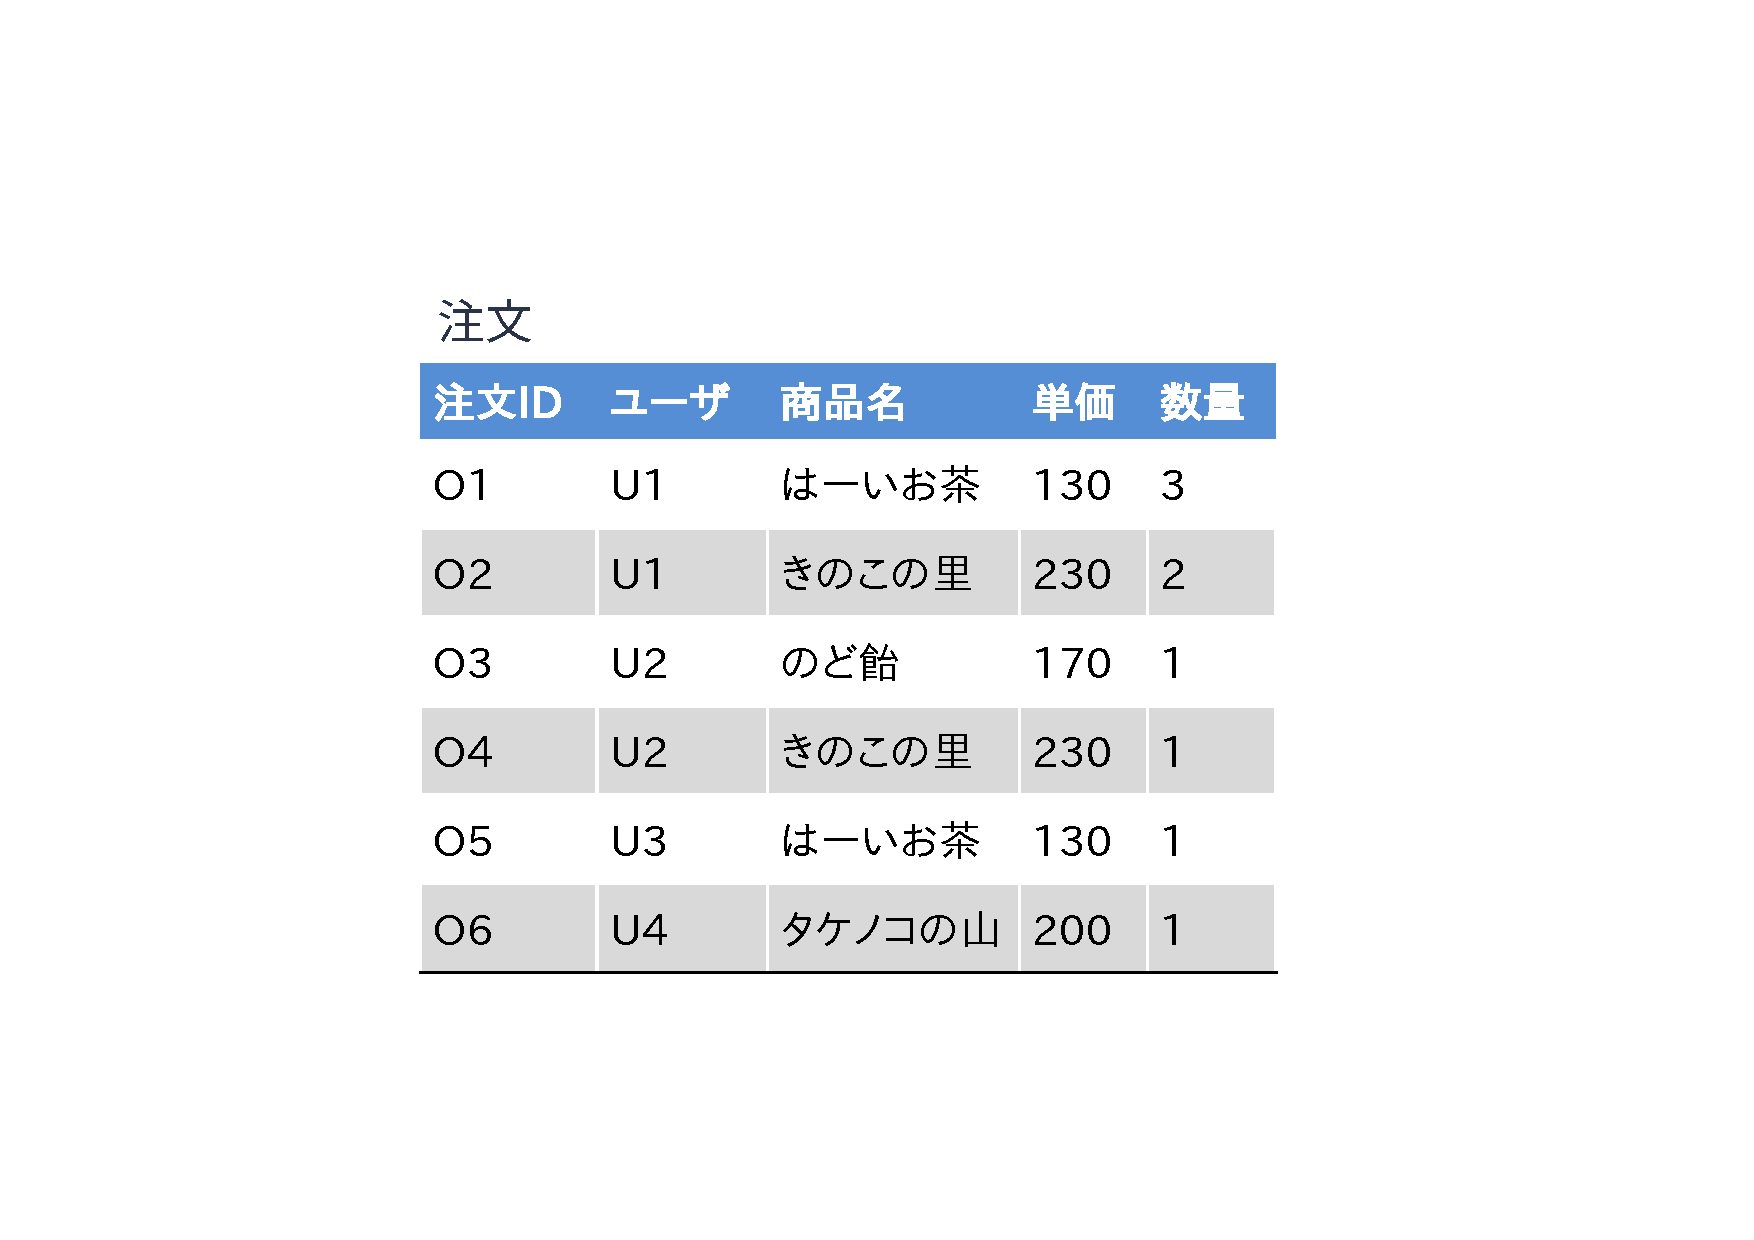
\includegraphics[width=0.7\textwidth]{figure/anomaly/order.pdf}
  \caption{ある時点までに蓄積された「注文」テーブル}
  \label{fig:order}
\endfigure

さて，山畑さんのショッピングサイトでは，新商品として\graybox{たきのこの里山}の取り扱いを開始することになりました．
新商品の情報をデータベースに登録するために，山畑さんは図\ref{fig:insertion-anomaly}のように「注文」テーブルに\graybox{(NULL, NULL, 'たきのこの里山', 250, NULL)}というレコードを追加しようとします．
ところが，RDBMSからデータの登録を拒否されてしまいました．
理由は，関係「注文」のスキーマにおいては\graybox{注文ID}が主キーとして設定されているからです．
まだ誰も注文していない\graybox{たきのこの里山}には\graybox{注文ID}が割り当てられていません．
そのため，主キーの値がないレコード\graybox{(NULL, NULL, 'たきのこの里山', 250, NULL)}はキー制約違反となって追加できないのです．
誰かが新商品を注文してくれないと新商品の情報をデータベースに登録できないとは，なんと不便なことでしょう．
山畑さんは「まだ誰も注文していない新商品」を登録できず，困ってしまいました…
\figure[tb]
  \centering
  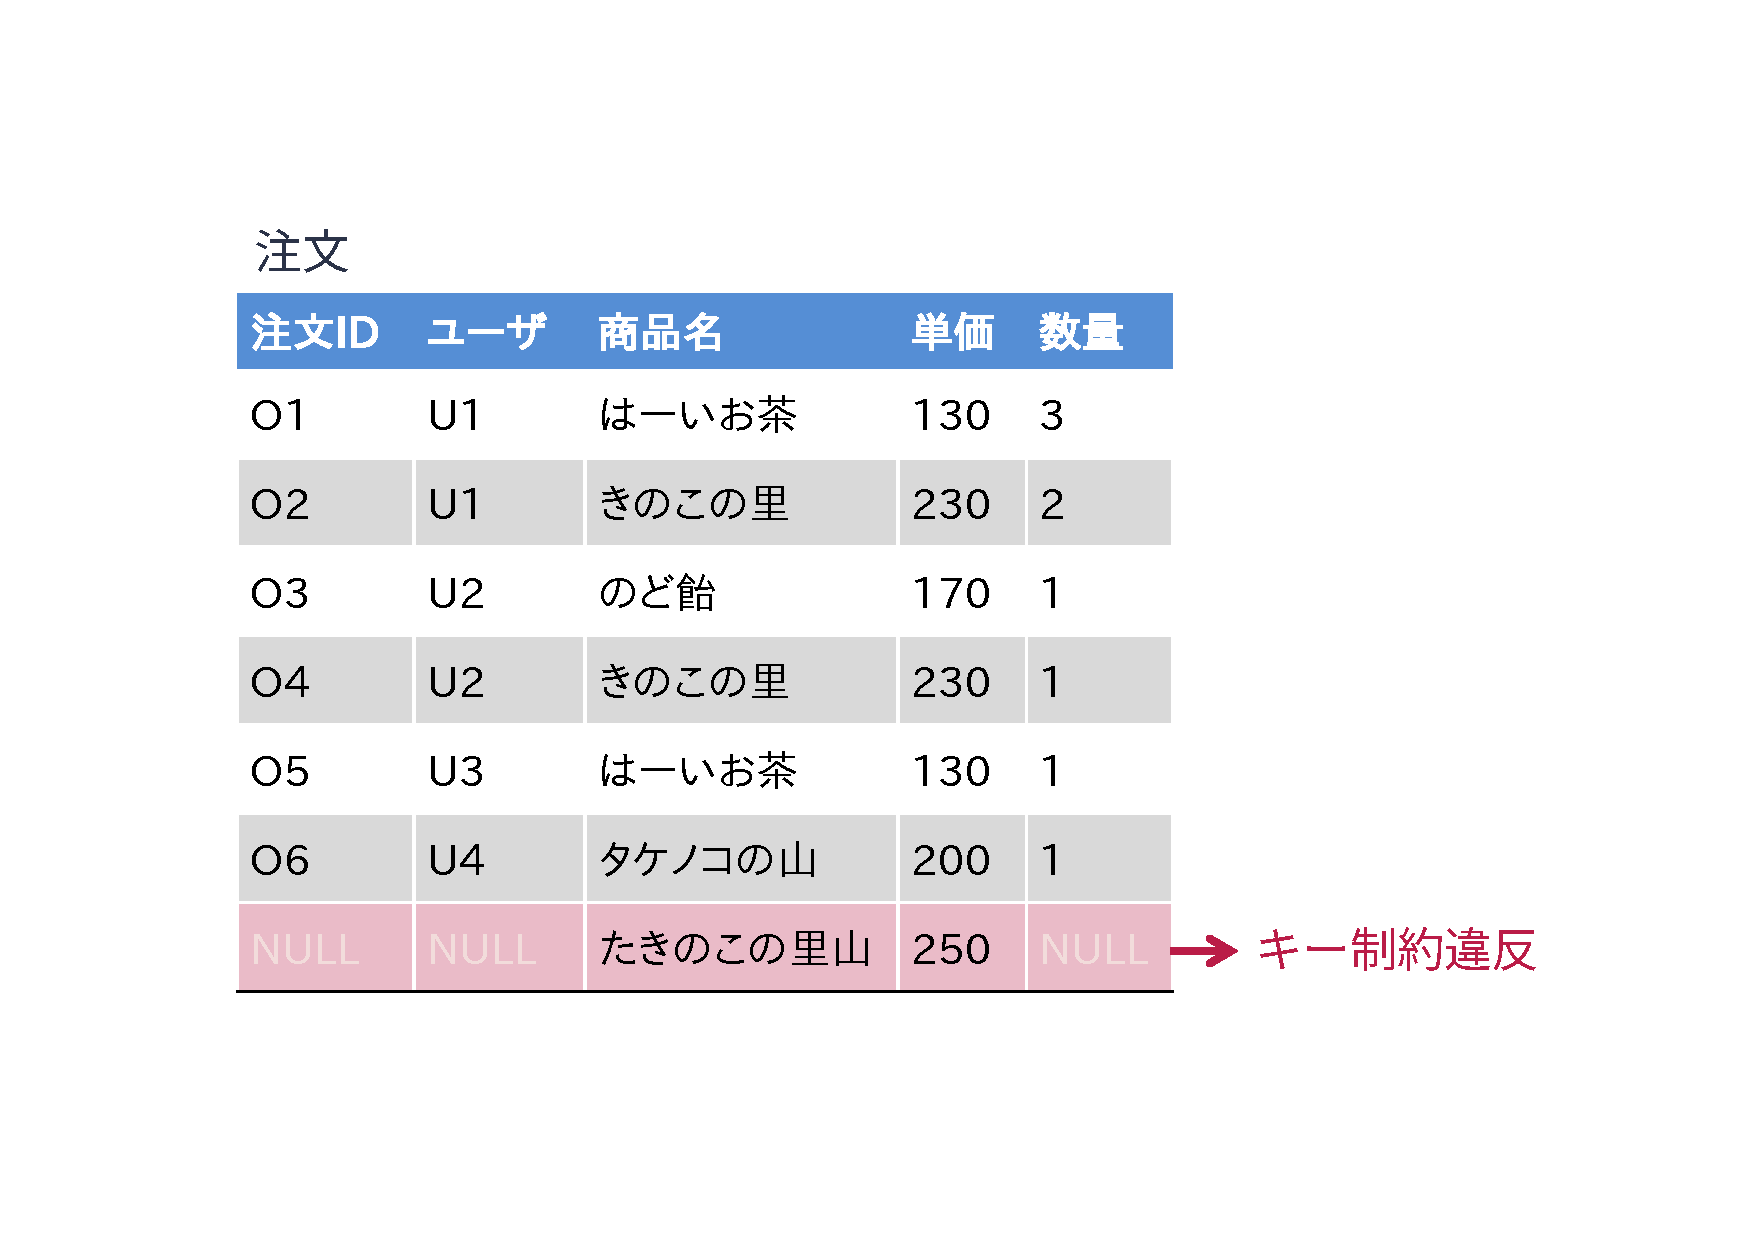
\includegraphics[width=0.9\textwidth]{figure/anomaly/insertion-anomaly.pdf}
  \caption{挿入時異状の例}
  \label{fig:insertion-anomaly}
\endfigure
このように，特定のレコードを挿入しようとしたときに，必要なデータが存在しないためにレコード登録ができない不都合な状態を\strong{挿入時異状（insertion anomaly）} と呼びます．



\section{削除時異状}
次に，図\ref{fig:order}のテーブルにおいて注文実績が1件しか存在しない\graybox{のど飴}について，ユーザ\graybox{U2}が払い戻しを希望したため，テーブルから関連する記録を削除しようとしているシーンについて考えてみましょう．
このとき，\strong{削除時異状（deletion anomaly）}と呼ばれる状態が発生します．

「注文」テーブルの設計の説明をした際，山畑さんはサイトで取り扱う商品についても「注文」テーブルの中で管理していると説明しました．
このような状況では，図\ref{fig:order}の3行目（注文IDが\graybox{O3}）のレコードを削除すると，図\ref{fig:deletion-anomaly}の状態になり，山畑さんのサイトで商品\graybox{のど飴}を取り扱っている事実や，商品の詳細情報（単価情報など）が意図しない形で失われてしまいます．
ユーザ\graybox{U2}は「注文をキャンセルしたかっただけ」なのに，サイト上は「\graybox{のど飴}という商品の存在そのものをデータベースから抹消してしまった」ことになります．
もし他のユーザが\graybox{のど飴}を買おうとしても，もうお店のサイトには並んでいない状態になってしまうのです．
このように削除時異状とは，あるレコードを削除したときに，残しておきたかった別の情報まで意図せずに消えてしまう状態を指します，
\figure[tb]
  \centering
  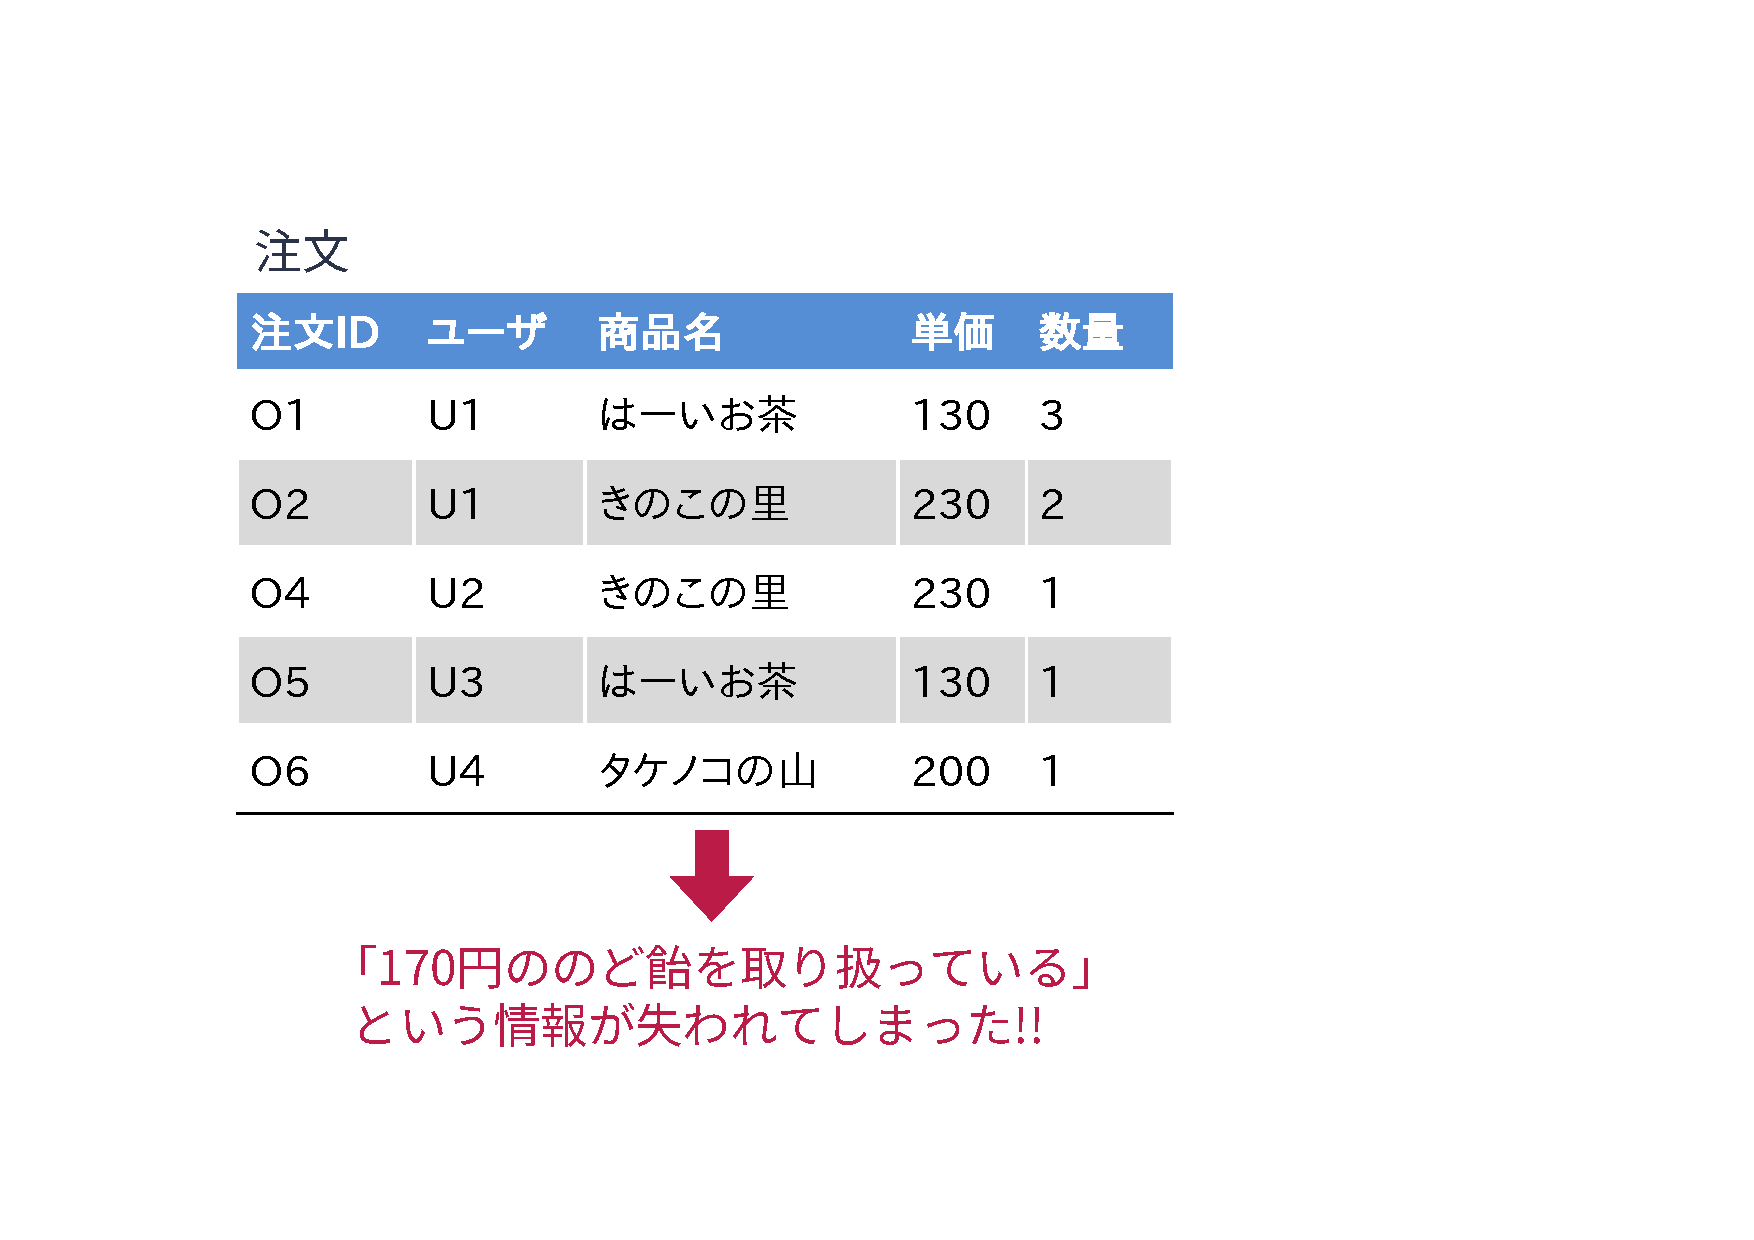
\includegraphics[width=0.8\textwidth]{figure/anomaly/deletion-anomaly.pdf}
  \caption{削除時異状の例}
  \label{fig:deletion-anomaly}
\endfigure

ところで，注文IDが\graybox{O3}のレコードを削除した後，山畑さんはのど飴の商品情報が消えてしまったことに気づいたとしましょう．
このとき，山畑さんが\graybox{(NULL, NULL, 'のど飴', 170, NULL)}というレコードを焦って追加して，\graybox{のど飴}の商品情報を復活させようとしても後の祭りです．
なぜなら，注文IDが存在しないため，このレコード追加しようとしても先に説明した挿入時異状が発生するからです．


\section{更新時異状}
3つ目の異状は\strong{更新時異状（update anomaly）}と呼ばれるものです．
例を見てみましょう．

図\ref{fig:order}のテーブルにおいて，\graybox{はーいお茶}の単価が\graybox{120円}であるにもかかわらず，山畑さんが勘違いして\graybox{130円}として注文テーブルに登録し続けていたとしましょう．
後日，山畑さんはこの誤りに気付きました．

さて，\graybox{はーいお茶}に関する注文は，注文IDが\graybox{O1}および\graybox{O5}の2件が該当します．
そのため，図\ref{fig:update-anomaly}のように，この2件の「単価」の値を\graybox{120}に書き換える必要があります．
ところが，山畑さんは該当商品の注文が1件しかないと思い込み，注文IDが\graybox{O1}のレコードの単価だけを修正し，\graybox{O5}の修正を忘れてしまいました．
ここで，山畑さんは「注文」テーブルの中でサイトの取扱商品も管理していたことを思い出してください．
先ほどのような修正忘れがあると，「注文」テーブルの中で同じ商品にも関わらず単価が異なる\graybox{はーいお茶}が存在することになり，どちらの単価が正しいのか分からない状態になってしまいます．
このように，一部のレコードの値を変更する際，更新漏れによるデータの矛盾が発生している状態を更新時異状と呼びます．
\figure[tb]
  \centering
  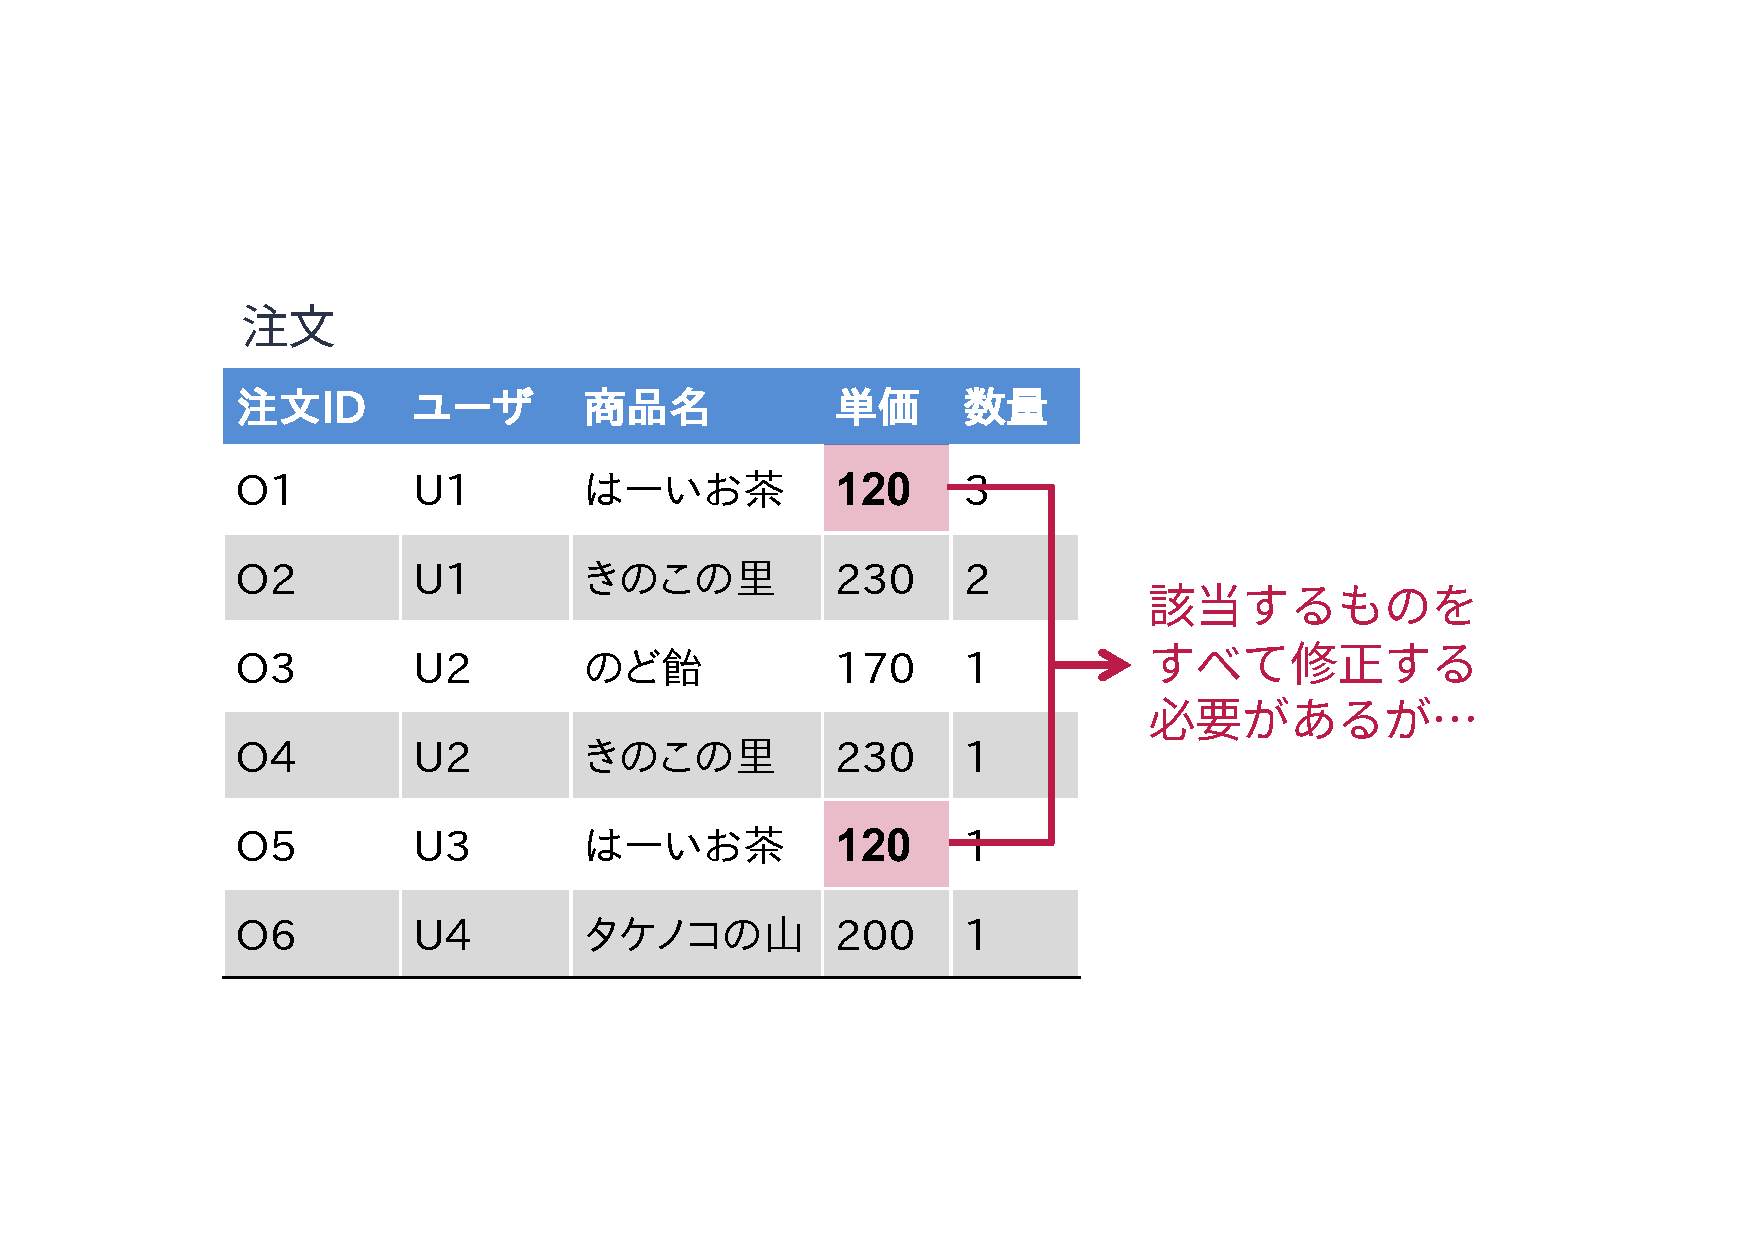
\includegraphics[width=0.9\textwidth]{figure/anomaly/update-anomaly.pdf}
  \caption{更新時異状の例}
  \label{fig:update-anomaly}
\endfigure

今回の例では「はーいお茶の単価が120円の間違いだった」という単一の商品に関する修正事象にもかかわらず，データベース上では2件のレコードの書き換え（修正）の必要がありました．
図\ref{fig:update-anomaly}の例では\graybox{はーいお茶}の注文履歴が2件しかありませんでしたが，修正対象となる履歴が100万件あれば100万回の修正が必要になります．
このように，データの重複が多いという状態は\strong{冗長性が高い}と表現されます．
データベースの冗長性が高いと，修正漏れが発生する可能性が高まるだけでなく，修正作業自体も非常に大変なものになってしまいます．


\section{異状を防ぐには}
上記のような「挿入時異状」「削除時異状」「更新時異状」が起きないようにするには，どうしたらよいのでしょうか．
\begin{itemize}
  \item 「注文」テーブルの中で商品情報も管理しているのが間違いなのでは…
  \item \ref{chap:sql-part1}章の説明で出てきた「商品」テーブルのように，商品の詳細情報を管理するためだけのテーブルを作ったら良いのでは…
\end{itemize}
このように考えた方は鋭いです．

山畑さんの「注文」テーブルの問題は，商品に関する属性を注文履歴と分けて扱えるにも関わらず，両者を同じテーブルの中で詰め込んで管理していることが原因でした．
山畑さんの異状問題を解決するためには，図\ref{fig:decomposition-example}のように，「注文」テーブルから商品に関する属性を切り離して，注文履歴とは別に商品情報を管理するための「商品」テーブルを作っておけばよかったのです．
このようにすれば，新商品である「たきのこの里山」を取り扱い商品に追加したい場合は，「商品」テーブルにそれに関するレコードを追加するだけで済み，挿入時異状が発生しません．
また，注文IDが\graybox{O3}のレコードを削除しても，「商品」テーブルの中の「のど飴」のレコードは残るため，削除時異状も発生しません．
「はーいお茶」の価格を変更する必要が生じても，「商品」テーブルの中の「はーいお茶」のレコードの「価格」を1箇所書き換えるだけで済むため，更新時異状も発生しません．
「注文」テーブルには商品の単価情報がありませんが，必要なときは「商品」テーブルを参照すれば，該当する商品の単価を知ることができます．
\figure[tb]
  \centering
  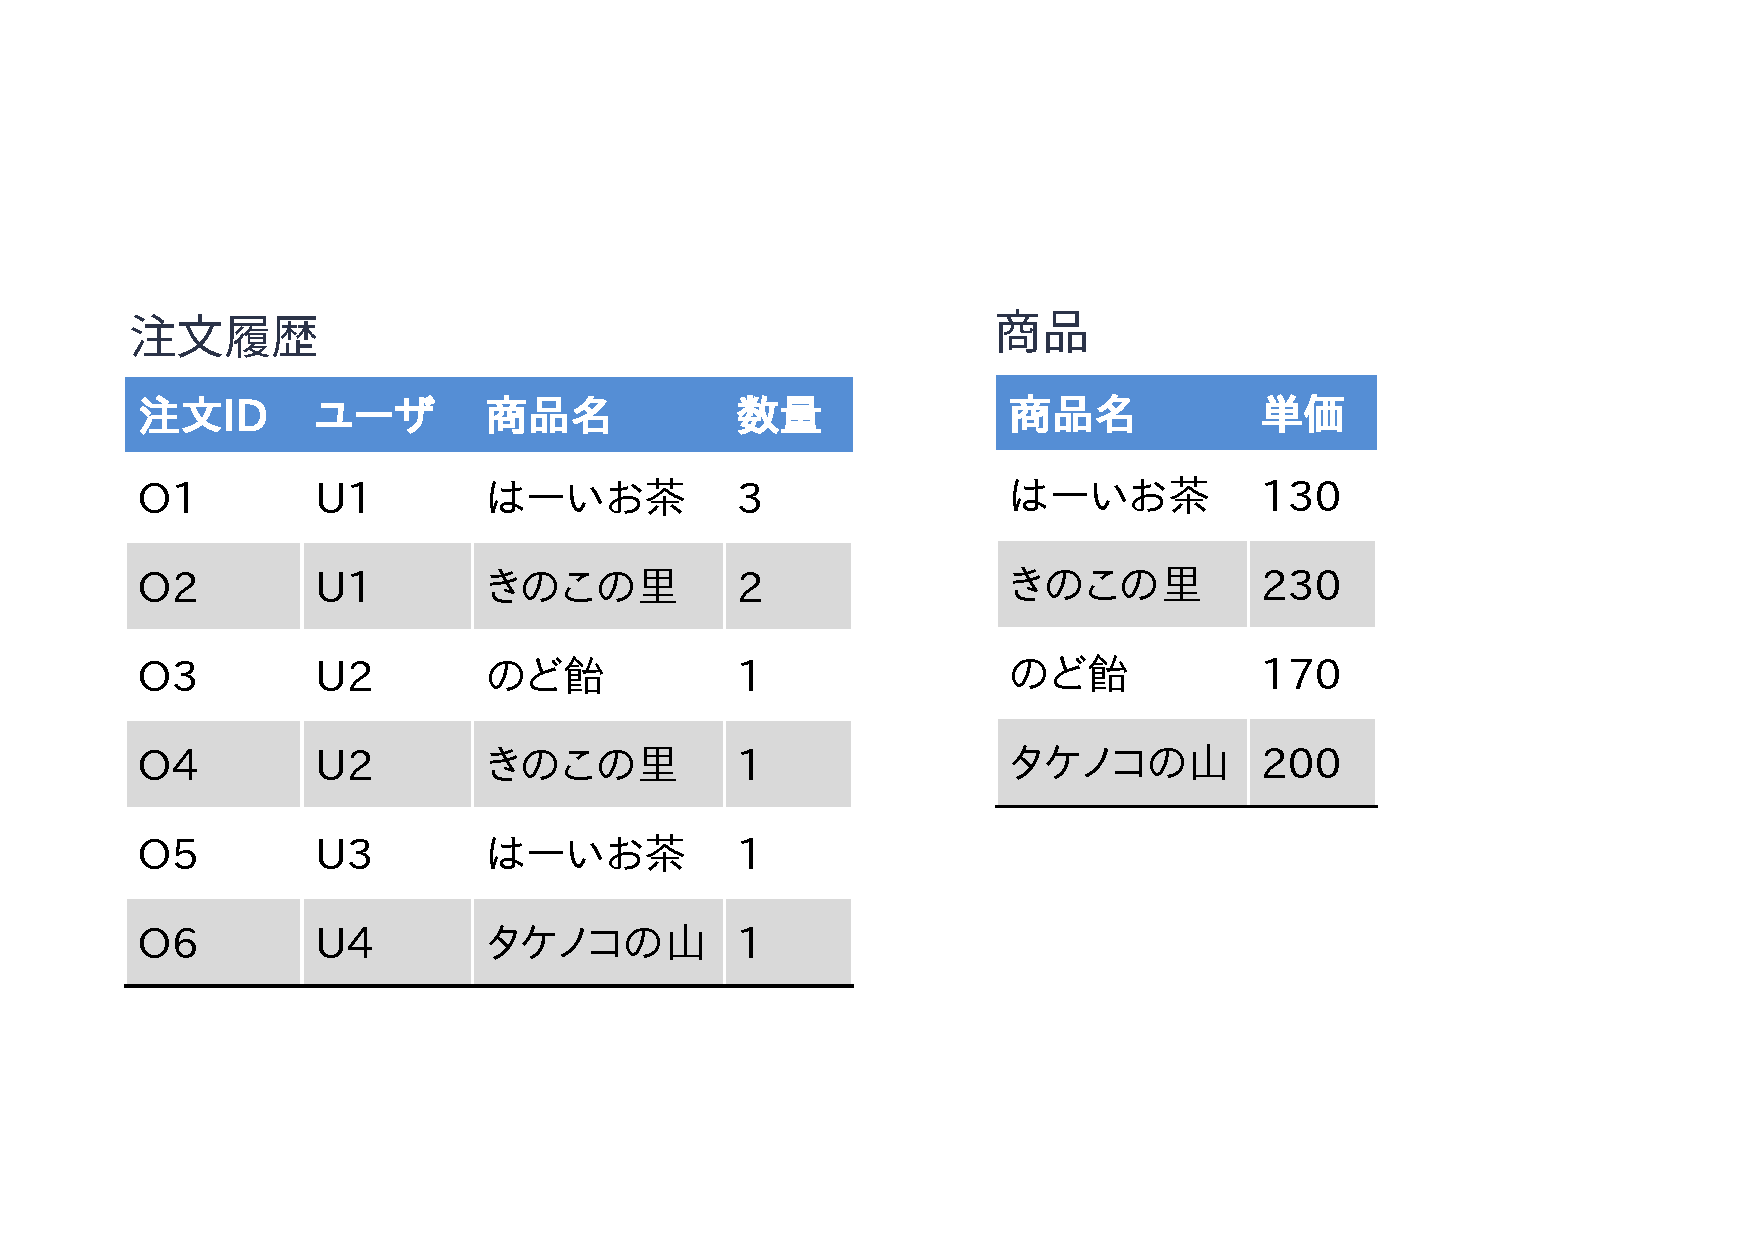
\includegraphics[width=0.9\textwidth]{figure/anomaly/decomposition-example.pdf}
  \caption{「注文」テーブルから商品に関する属性を切り離して「商品」テーブルを作ることによって異状を防ぐ例}
  \label{fig:decomposition-example}
\endfigure

このように，データベースの異状は関係スキーマ（テーブルの構造）を適切に設計することによって防ぐことができます\cite{Bernstein1976}．
今回の例では「注文」テーブルから商品に関する情報を切り出して「商品」テーブルを作ればよいということが直感的に分かりました．
しかし，実際のデータベースの設計においてはデータ間の関係が複雑であることも多く，テーブルの中で取り扱うべき属性情報を決めるのも簡単なことではありません．
そこで次章では，データを正しく矛盾なく保つための適切な関係スキーマの設計方法について学びましょう．


% ---------------------------------------
%\hrulefill
\section{クイズ}
% ---------------------------------------
\subsubsection{Q1. 異状の分類}
ある大学の授業システム上で，以下のような「履修登録」テーブルが作られました．
主キーは\graybox{\{学生ID, 科目ID}\}です．

\begin{equation*}
  \text{履修登録}(\underline{\text{学生ID, 科目ID}}, \text{学生名}, \text{科目名}, \text{担当教員})
\end{equation*}

このテーブルを運用していたところ，以下の(1)〜(3)のトラブルが発生しました．
それぞれ，「挿入時異状」「削除時異状」「更新時異状」のどれに該当するか答えなさい．
\begin{enumerate}
\item 科目「データサイエンス入門」が新設され，担当教員も決まったが，まだ誰も履修登録をしていないため，データベースに科目を登録できない．

\item「プログラミング基礎」という科目を担当していた教員が変わったため，この科目を履修している学生100人分のレコードすべての「担当教員」を書き換えなければならず，一部で修正漏れが発生した．

\item 「離散数学」という科目を履修していた唯一の学生が履修を取り消した（レコードを削除した）ところ，「離散数学」という科目が存在したこと，誰が担当教員だったのかという情報までデータベースから消えてしまった．
\end{enumerate}


\subsubsection{Q2. 更新時異状}
架空の家具販売店「八高家具」では顧客と購入希望商品の「ペア」（誰が何の商品の購入を希望しているか）で営業担当を割り当てています．
営業担当は年度ごとに営業成績が評価されることになっています．

八高家具では，下記関係スキーマに従った関係データモデルを用いて営業記録，取扱商品，営業成績の管理を行っています．
\begin{equation*}
  \text{営業記録}(\underline{\text{ユーザ}}, \text{商品}, \text{連絡先}, \text{メーカー}, \text{営業担当}, \text{営業成績})
\end{equation*}

図\ref{fig:sale-history}は，関係スキーマ「営業記録」にしたがって八高家具における営業記録を記録したテーブルです．
営業担当者の成績の修正に際して，関係「営業記録」のみを用いてデータを管理する際に発生しうる更新時異状の例を挙げなさい．
\figure[htb]
  \centering
  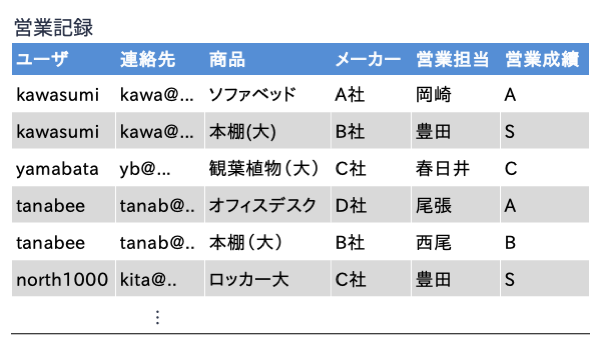
\includegraphics[width=0.7\textwidth]{figure/anomaly/sale-history.png}
  \caption{八高家具の「営業記録」テーブル}
  \label{fig:sale-history}
\endfigure


\subsubsection{Q3. 削除時異状}
架空の家具販売店「八高家具」では，以下のような修正した関係スキーマを用いて，改めて営業記録をつけ始めました．
\begin{equation*}
  \text{営業記録2}(\underline{\text{ユーザ}, \text{商品}}, \text{連絡先}, \text{メーカー}, \text{営業担当})
\end{equation*}

図\ref{fig:sale-history2}は，関係スキーマ「営業記録2」にしたがって営業記録を記録したテーブルです．
営業担当者の成績の修正に際して，関係「営業記録2」のみを用いてデータを管理する際に発生しうる削除時異状の例を挙げなさい．
\figure[htb]
  \centering
  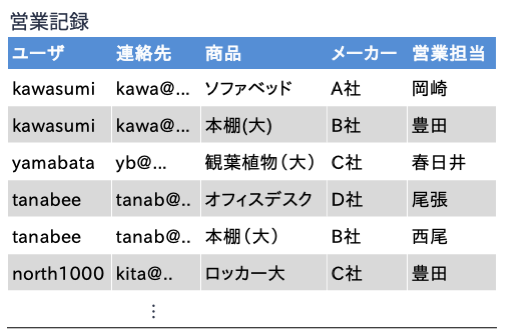
\includegraphics[width=0.7\textwidth]{figure/anomaly/sale-history2.png}
  \caption{八高家具の「営業記録2」テーブル}
  \label{fig:sale-history2}
\endfigure


\subsubsection{Q4. 挿入時異状}
架空の家具販売店「八高家具」では，更に修正した以下の関係スキーマを用いて改めて営業記録をつけ始めました．
\begin{equation*}
  \text{営業記録3}(\underline{\text{ユーザ}, \text{商品}},  \text{メーカー}, \text{営業担当})
\end{equation*}

図\ref{fig:sale-history3}は，関係スキーマ「営業記録3」にしたがって営業記録を記録したテーブルです．
営業担当者の成績の修正に際して，関係「営業記録3」のみを用いてデータを管理する際に発生しうる挿入時異状の例を挙げなさい．
\figure[htb]
  \centering
  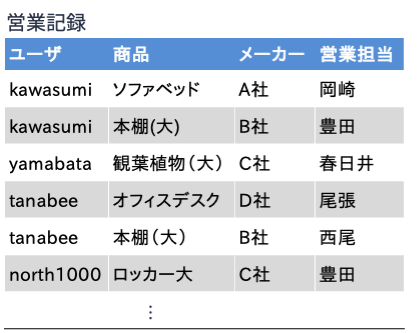
\includegraphics[width=0.7\textwidth]{figure/anomaly/sale-history3.png}
  \caption{八高家具の「営業記録3」テーブル}
  \label{fig:sale-history3}
\endfigure



% \chapter{関係データベースの設計 -- 実体関連モデル}\label{chap:er-model}

\ref{chap:anomaly}章では，データの挿入，削除，更新時に発生するデータベースの不都合である異状について説明しました．
データベースの異状を含め，データベースが常に正しく矛盾がない状態に保つためには，\ref{chap:relational-data-model}章で説明した関係データモデルの制約やテーブルの構造を適切に設計することが重要になってきます．

ところが，データベースを正しく設計することは想像以上に難しいことです．
これまでの章で説明に用いてきたテーブルは高々2，3個でした．
しかし，データ管理の現場では関係データベース内のテーブルの数が数十，数百になることはめずらしくありません．
また，データベース設計においては唯一の正解があるわけではなく，現実世界の複雑なルールやデータが用いられる文脈を紐解き，それをデータベース管理システムが扱える形に落とし込む必要があります．
そのため，どれほど経験があるデータエンジニアであっても，いきなり完全無欠でメンテナンスもしやすい関係データベースを設計することは難しいです．
データが正しく保たれ，冗長なデータも発生せず，かつ一貫性制約の保持が容易である関係データベースを設計するには，対象とする事象やその中に存在するルールに対する理解を深めた上で，体系的にデータモデルを構築する必要があります．

そこで本章および次章では，関係データベースの設計手法である\strong{実体関連モデルを変換する方法}および\strong{正規化}について解説します．


\section{データモデリングの流れ}
\ref{chap:concept-of-database}章で説明したように，データモデリングとは対象とする課題に応じて扱うべき情報を取捨選択し，データの構造，制約条件，操作方法を設計する行為です．
図\ref{fig:data_modeling_process}が示すように，一般にデータモデリングは概念モデリング，論理モデリングの順で行われます．
\begin{figure}[tb]
    \centering
    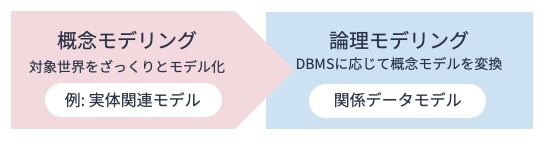
\includegraphics[width=0.8\textwidth]{figure/er-model/data-modeling-process.jpg}
    \caption{データモデリングの流れ}
    \label{fig:data_modeling_process}
\end{figure}

\strong{概念モデリング}は，最終的にどのようなデータベース技術を利用するかに関係なく，対象とする課題（例：ビジネスの業務要件）の全体像を把握した上で，扱おうとするデータ対象がどのようなものであるか（どのような意味を持つか）を記述する手続きです．
概念モデリングにおいては，本章で説明する実体関連モデルが用いられることが多いです．

\strong{論理モデリング}の過程では，概念モデリングで設計された概念モデルをデータベース管理システムが扱えるよう変換します．
例えば，データベース管理システムが関係データベース管理システムであれば，あらかじめ設計された概念モデルを関係データモデルに変換することになります．


本書では関係データベースの設計手法として，実体関連モデルに基づく方法と関数従属性にもとづく正規化の2種類の方法を学びます．
これらは二者択一ではなく，両方を組み合わせて用いることが実務におけるベストプラクティスです．
詳細は本章，次章で説明しますが，それぞれの利用シーンは以下の通りです：
\begin{description}
    \item[実体関連モデルに基づく方法]：何もない状況から対象課題の要件を整理し，データの構造や関連を俯瞰的に設計したい場合
    \item[データ従属性にもとづく正規化]：ある程度具体的なデータ項目（テーブルの属性）が出揃っている状況で，データの重複や異状が発生しないテーブル構造を導出したい場合
\end{description}

以降本章では，代表的な概念モデルである実体関連モデルを解説した後，実体関連モデルを関係データモデルに変換する方法について述べます．


\begin{notebox}{データモデリングは難しい!?}
本章および次章では「データベースの設計方法」を学びますが，学ばなければならない知識はそれほど多くありません．
例えば，本章で学ぶ実体関連モデルでは，主要概念は「実体」と「関連」の2種類しかありません．
内容も一見すると，大したことがないように見えます．
ところが，実際にデータベース設計ができるようになるには時間がかかります．
例えば，実体関連モデルの概念を学んだ初心者がいざ実体関連モデルを作ろうとすると，何をどうすればよいのか困るでしょうし，モデルを作ったもののそれが正しいものか不安になるでしょう．
設計は知識よりも経験（考え方の体得）がものを言うからです．
データモデリングのような抽象的な思考を体得するには，とにかく「やってみては間違えるを繰り返す」しかありません．
\end{notebox}



\section{実体関連モデルとは}
\strong{実体関連モデル（entity-relationship model; ERモデル）} は，Peter Chenにより提唱された概念モデリング用のデータモデルです\cite{Chen1976}．
実体関連モデルでは，実世界のデータのすべてを「実体」と「関連」の2種類で分類・記述します．
実体関連モデルを図として表現したものを\strong{実体関連図（entity-relationship diagram; ER図）} と呼びます．

実体関連モデルおよび実体関連図には様々な記法\footnote{本書で説明するPeter Chen記法以外には，カラス足記法，IDEF1X記法などが存在します．}・拡張が存在します\cite{Batini1991}が，本書ではPeter Chenの記法に従い説明を行います．

\subsection{実体}
\strong{実体（entity）}とは，データ対象をモデル化しようとしたときに，独立した存在として一意に識別可能な物体や事象です．
例えば，ショッピングサイトで取り扱う商品や購買記録をデータベースで管理することを考えてみましょう．
そこに登場する個々のゆーザや商品，販売者，商品レビュー，カートなどはすべて実体と見なせます．
なお，商品レビューやカートは物理的に存在するものではありませんが，概念的には独立した存在として識別可能な事象であるため実体となりえます．

同じ種類の実体の集合を\strong{実体集合}と呼びます．
実体集合と実体は「集合とその要素（インスタンス）」の関係になります．
例えば，
\begin{itemize}
 \item 実体集合「ユーザ」の要素（つまり実体）としては，「ユーザA」「ユーザB」「ユーザC」など
 \item 実体集合「商品」の要素（つまり実体）としては，「はーいお茶」「午前の紅茶」「健康麦茶」など
\end{itemize}
が考えられます．

実体集合の属性や一貫性制約を定めたものを\strong{実体型（entity type）}と呼びます．
実体型の実体の「ひな形」のようなものです．．
実体型は必ず1つ以上の\strong{属性（attribute）}を持ちます．
属性とは実体を特徴づける性質を表すものです．
例えば，実体集合「商品」の属性としては「商品ID」「商品名」「価格」「発売日」などが挙げられます．

関係データモデルと同様，実体集合の実体（要素）を一意に識別（特定）するための極小な属性集合を\strong{キー}と呼びます．
例えば，先の実体集合「商品」が「商品ID」という属性を持ち，どの実体「商品」も異なる「商品ID」を持つのであれば，「商品ID」はキーとなります．
キーのうち，管理上最適と考えられるものを\strong{主キー}と呼びます．
実体型は\strong{必ず主キーを持ちます}．
つまり，実体は実体集合内で必ず一意に識別できる必要があります．

Peter Chenの記法では，実体関連図において，
\begin{itemize}
\item 実体型は矩形
\item 属性は楕円
\end{itemize}
実体型とその属性は線で結びます．
また，主キーとなる属性には\strong{下線を引きます}．

図\ref{fig:product_entity}は，あるショッピングサイトにおける実体型「商品」を実体関連図として表現したものです．
仮にこのような実体型「商品」を設計したとすると，このショッピングサイトで取り扱うすべての商品は必ず「商品ID」「商品名」「価格」「発売日」を属性として持つ（そして，これら以外の属性は持たない）ことがルールとして定められたことになります．
\begin{figure}[htb]
    \centering
    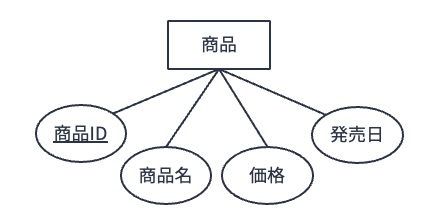
\includegraphics[width=0.7\textwidth]{figure/er-model/product-entity.jpg}
    \caption{実体型「商品」の実体関連図}
    \label{fig:product_entity}
\end{figure}

\begin{notebox}{「一意に識別できる」とは？}
実体や関連の定義において「一意に識別（特定）できる」という言い回しが頻繁に使われます．
「事柄Xが（ある集合内において）一意に識別できる」とは「集合内に事柄Xとまったく同じものがなく，集合の中からXをピタリと特定できる」という意味です．

例えば実体型「商品」において「商品ID」が主キーとなっている場合，商品集合内の各商品は「（商品IDをもって）一意に識別できる」と言えます．
これは「商品IDを見れば，（他の商品と区別して）ある商品を唯一1つに絞り込むことができる」という意味になります．
言い換えれば，実体集合「商品」においては，まったく同じ「商品」は存在しない（してはいけない）という意味になります．
\end{notebox}


\subsection{関連}
\strong{関連（relationship）}とは，複数の実体間のつながりを表します\footnote{「関連」と「関係」は混同しやすいが異なる概念なので注意すること．「関連（relationship）」は実体関連モデルにおける概念で，複数の実体間のつながりを表します．一方，「関係（relation）」は数学や関係データベース上の概念で，集合の直積の部分集合を意味します．}．
例えば，Amazonなどのショッピングサイトでしばしば提供されている，欲しい（購入希望の）商品をリスト化しておく「ウィッシュリスト（お気に入り）」機能について考えてみましょう．
これを実体関連モデルで表現するならば，実体「ユーザ」と実体「商品」の間に「お気に入り」という関連を定義することができます．
関連は，結びつく実体（ユーザや商品など）が存在して初めて意味を持ちます．
例えば，先に挙げた関連「お気に入り」について，お気に入り（として登録する）という行為は行為主体であるユーザと行為対象である商品がそろって初めて定義できます．

同じ種類の関連の集合は\strong{関連集合（relationship set）}と呼ばれます．
例えば，先の「お気に入り」の例では，
\begin{itemize}
\item ユーザAが商品Xをお気に入り登録したこと
\item ユーザBが商品Yをお気に入り登録したこと
\end{itemize}
など，個々のユーザが何かをお気に入り登録したという行為の集合が関連集合「お気に入り」となります．
% 関連集合内の各関連は，それとつながっている複数の実体によって「一意に識別」されます．
% 言い換えると，ある関連はそれとつながっている実体の主キーの値が指定されたとき，一意に識別されなければなりません．
% これは非常に重要かつ分かりにくいポイントです．

関連型も属性を持つ場合があります（属性がないこともあります）．
例えば，先の関連型「お気に入り」の例であれば，サイトにお気に入りを登録した「登録日」などが属性として考えられます．

Peter Chenの記法では実体関連図において，
\begin{itemize}
\item 関連型はひし形
\item その属性は楕円
\end{itemize}
で表現されます．
関連型とその属性は線で結び，関連型はつながりのある実体型と線で結びます．

図\ref{fig:wishlist_relationship}は，実体型「ユーザ」「商品」，および関連型「お気に入り」を実体関連図として表現したものです．
\figure[htb]
    \centering
    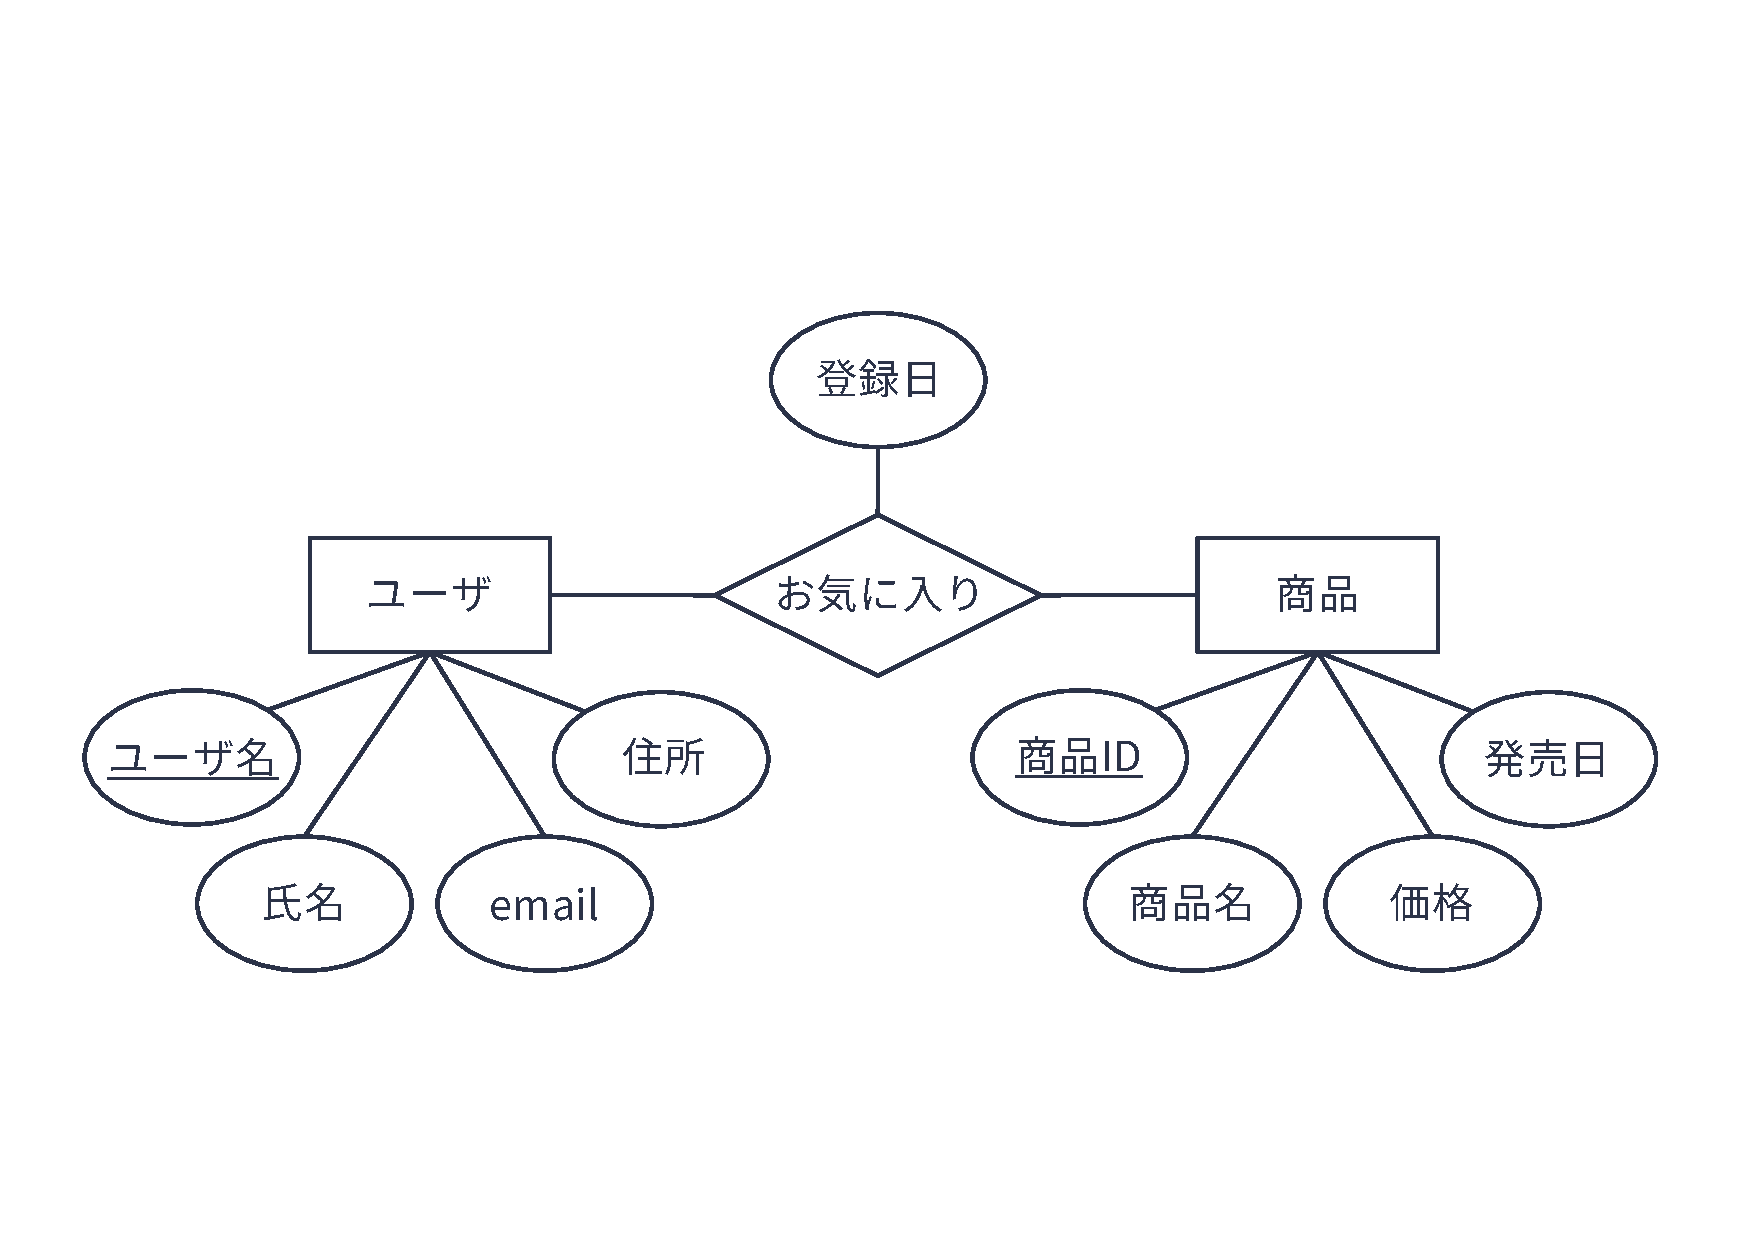
\includegraphics[width=0.85\textwidth]{figure/er-model/wishlist-relationship.pdf}
    \caption{実体型「ユーザ」「商品」と関連型「お気に入り」の実体関連図}
    \label{fig:wishlist_relationship}
\endfigure

実体は実体集合内で一意に識別できる必要があると述べましたが，関連も関連集合内で一意に識別できる必要があります．
もう少し具体的に言うと，ある関連はそれとつながっている実体の主キーの値が指定されたとき，一意に識別されなければなりません．
実際，実体関連モデルにおける関連は，数学的には「実体の主キーの組み合わせ」として扱われます．
これは非常に重要ですが，分かりにくいポイントでもあるので，例を挙げて考えてみましょう．

図\ref{fig:er_model_elements}は，上の実体関連図に示したモデルの実体および関連（つまり実体集合および関連集合の要素）の例を図示したものです．
ベン図において，点は各集合の要素（つまり実体や関連）を表しています．
実体「ユーザ」「商品」の点の下に書かれた値は，ある実体の主キーの値を示しています．
また，関連「お気に入り」の下に書かれた値は，各関連につながる実体の主キーの値のペアを示しています．
例えば，真ん中の\graybox{(U1,P1)}の点は，ユーザ\graybox{川澄}（主キーは\graybox{U1}）が商品\graybox{はーいお茶}（主キーは\graybox{P1}）をお気に入り登録したことを表しています．
このように，一つ一つの関連「お気に入り」は実体「ユーザ」と「商品」の主キーのペアで表現されます．
それによって，「ユーザ」の主キーと「商品」の主キーの値が指定されれば．どの関連「お気に入り」かを一意に識別できるようになっています．
すでに説明したように，関連集合の要素は一意に識別できる必要があります．
そのため，図の赤バツ印の箇所のように，ユーザ\graybox{川澄}が商品\graybox{はーいお茶}を2回目のお気に入り登録することできません．
関連集合は「集合」であるため，\graybox{(U1,P1)}のような同じ値の要素を複数持つことはできないのです．
この実体関連モデルでは，ユーザは同じ商品に対するお気に入りを1回分しか登録できないことになります．
あるユーザの同じ商品に対する複数回のお気に入りを別々に扱いたい場合は，モデリングを工夫する必要があります（これについては，後ほど説明します）．
\figure[htb]
    \centering
    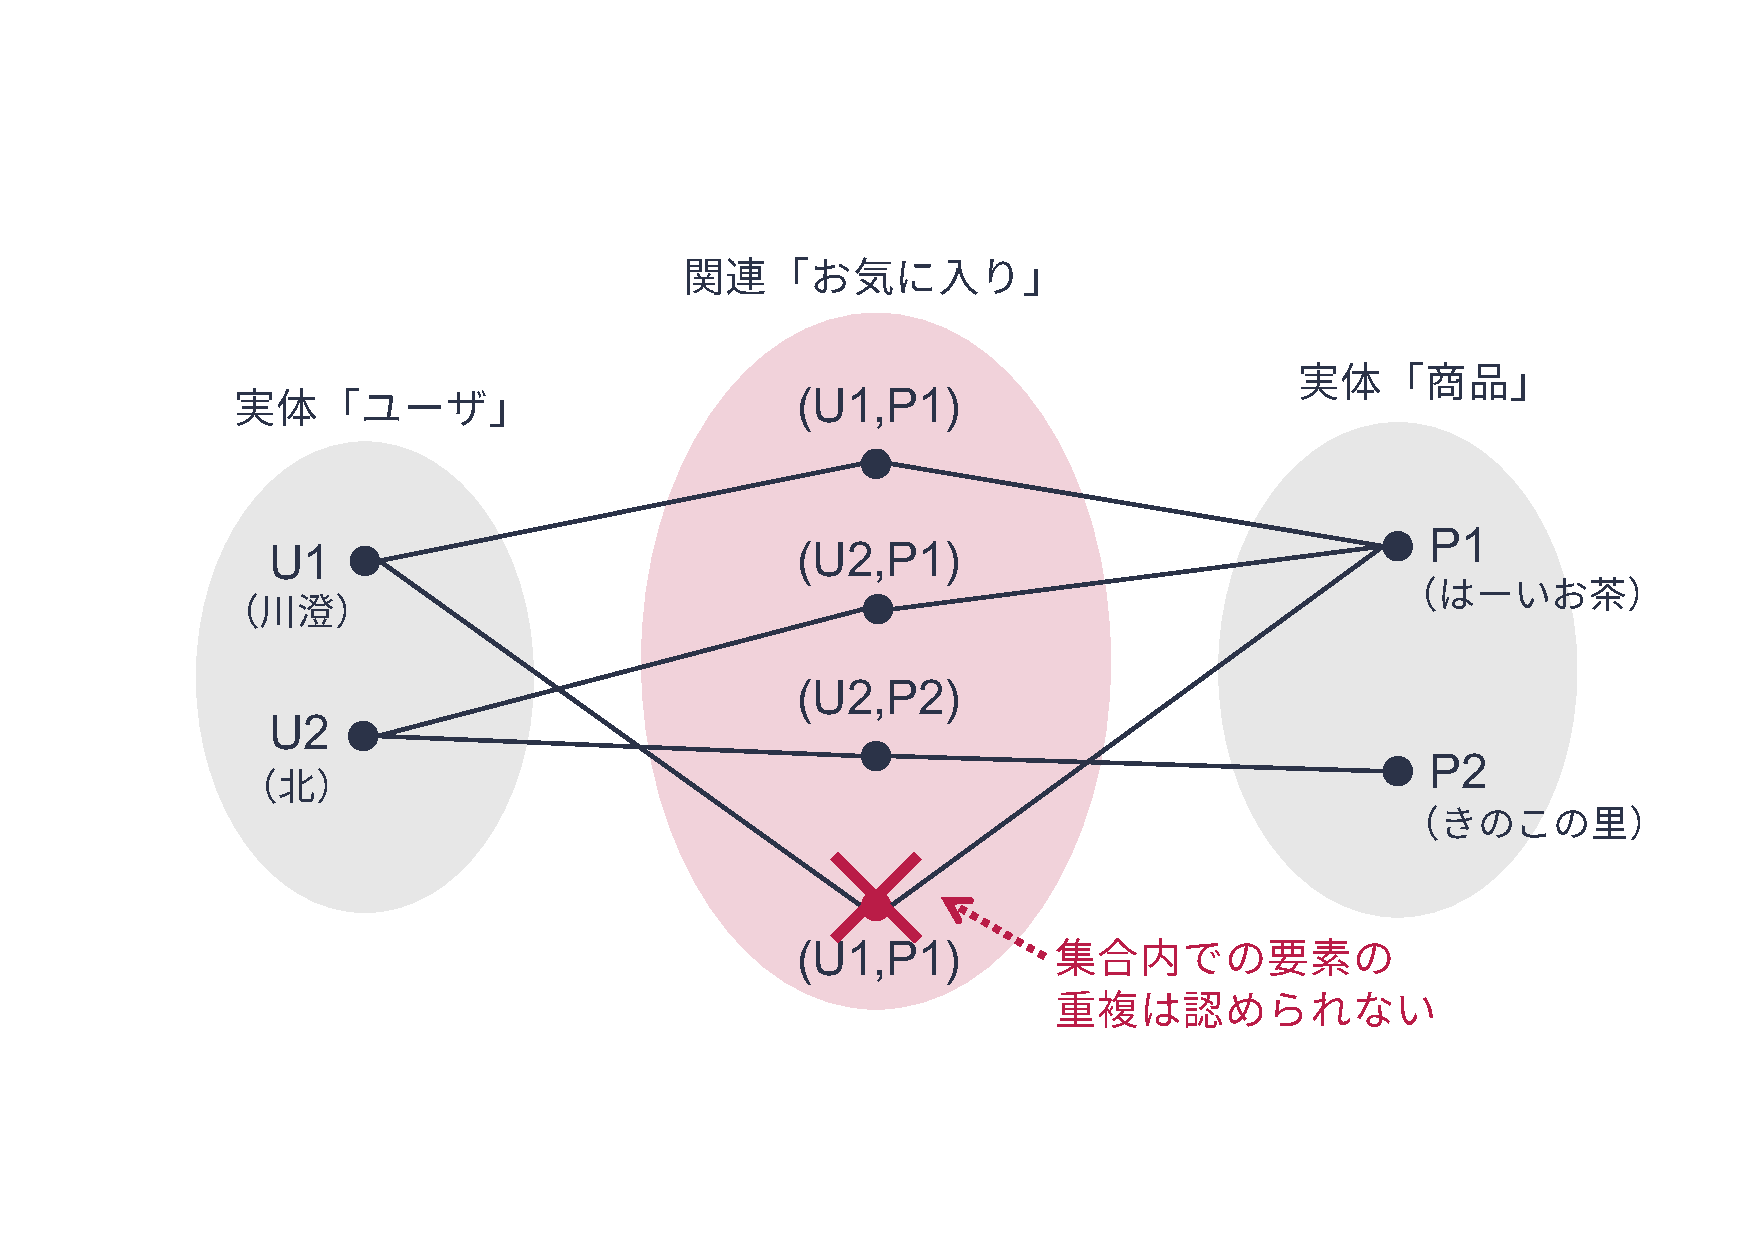
\includegraphics[width=0.85\textwidth]{figure/er-model/er-model-elements.pdf}
    \caption{実体型「ユーザ」「商品」と関連型「お気に入り」の実体集合および関連集合の要素の例}
    \label{fig:er_model_elements}
\endfigure



\subsection{役割の明示}
ある大学ではデータベースを用いた学生情報の管理を検討しています．
さて，この大学ではどの学生も
\begin{itemize}
\item 自分の面倒を見てくれる「先輩」学生
\item 面倒を見てあげる必要のある「後輩」学生
\end{itemize}
が割り当てられているとします．
このような状況を実体関連モデルで表現することを考えてみましょう．

与えられた条件をふまえて
\begin{itemize}
\item 実体型として「先輩学生」と「後輩学生」，
\item 先輩学生と後輩学生とのつながりを表す関連型として「世話」
\end{itemize}
を定義したとしましょう．
この定義に従ってデータを管理しようとすると，面倒なことが起きます．

例えば，山畑滝子さんという学生には，川澄桜子さんという先輩と田辺通さんという後輩がいたとしよう．
この状況を先に定義した実体関連モデルで考えてみると，図\ref{fig:er_model_without_role}のように，\graybox{山畑滝子}という唯一無二の実体が実体集合「先輩学生」と実体集合「後輩学生」のそれぞれの要素に現れてしまいます．
検討しているデータベースでは学生情報を管理したいので，2つの実体集合に同じ情報が二重に登場するのは冗長で望ましくありません．
先の実体関連モデリングは適切ではなかったのです．
\begin{figure}[htb]
    \centering
    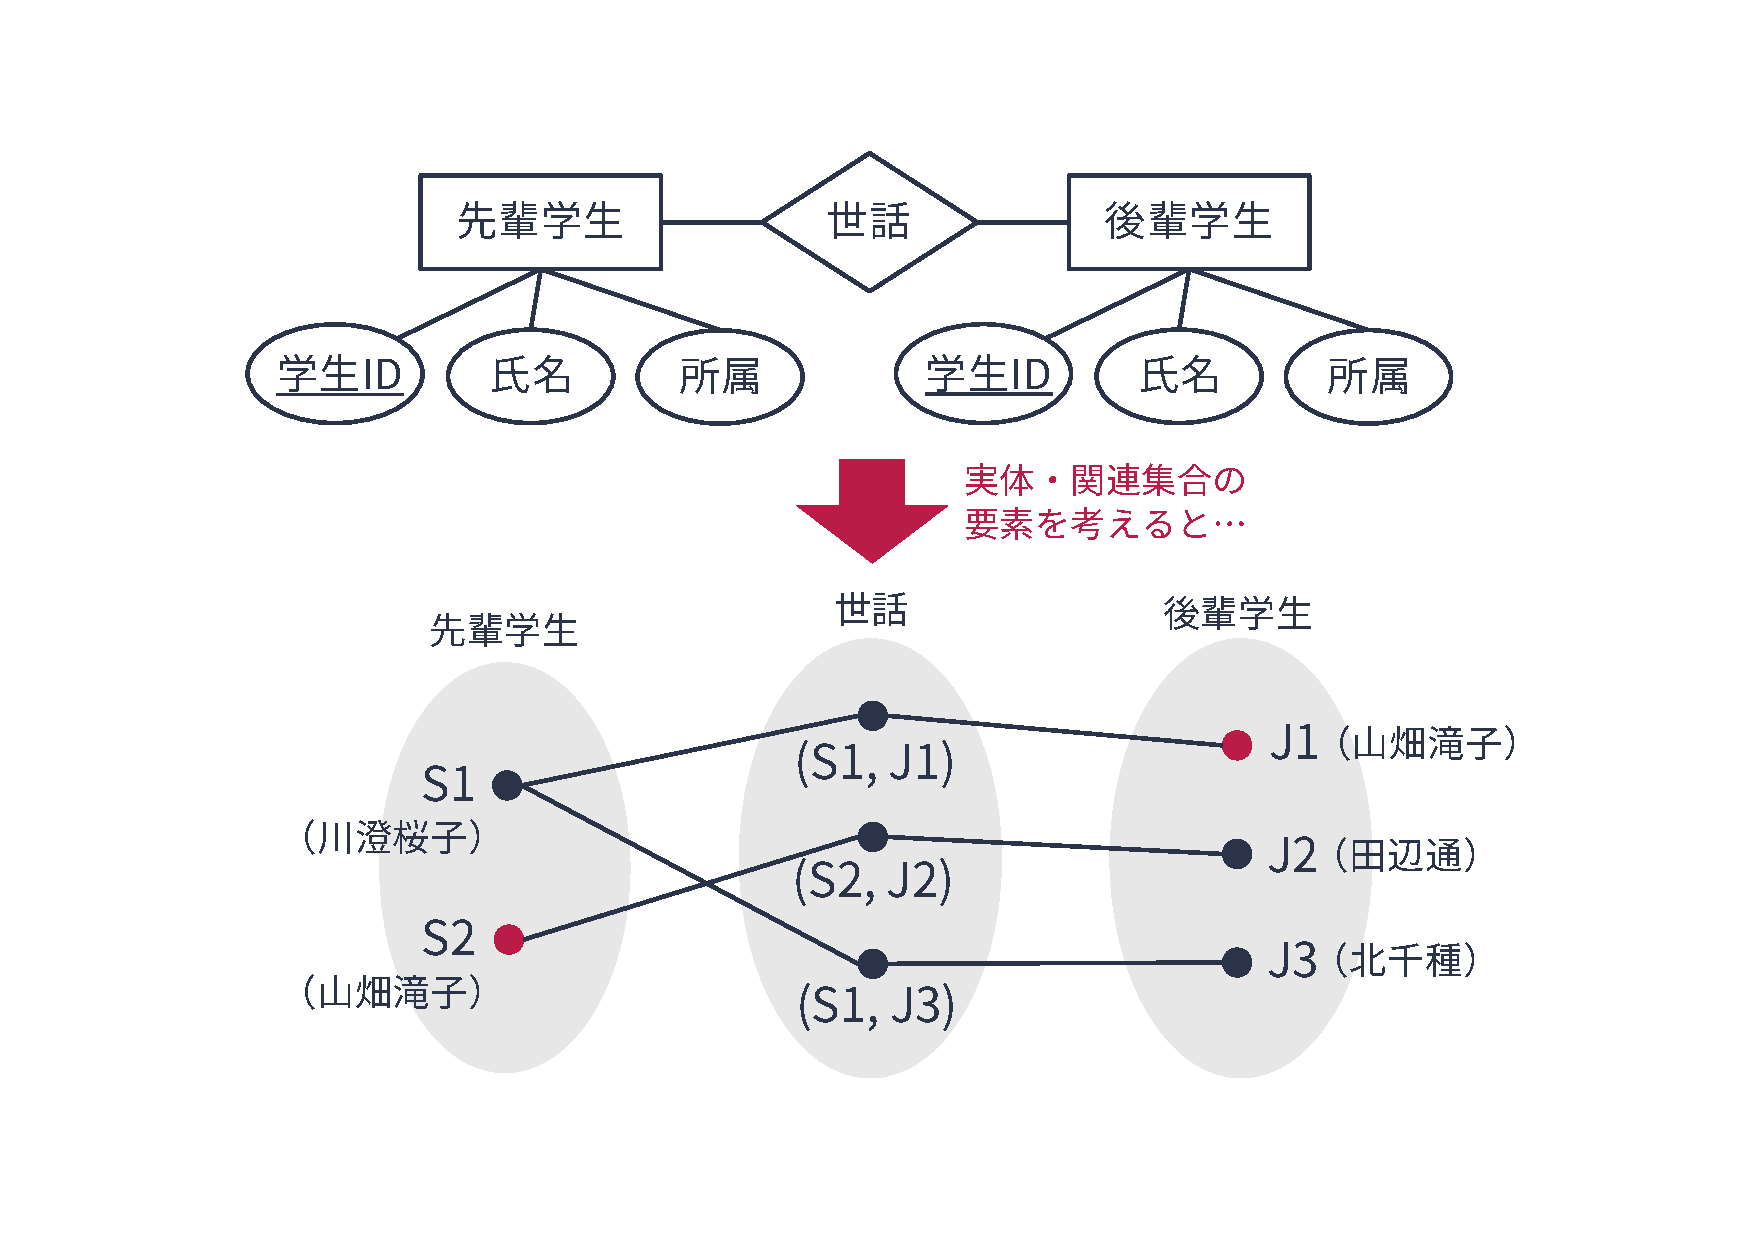
\includegraphics[width=0.8\textwidth]{figure/er-model/er-model-without-role.pdf}
    \caption{役割を明示しない実体関連図の例．分かりやすさのために，要素の隣には属性「名前」の値を記載している．}
    \label{fig:er_model_without_role}
\end{figure}

先輩学生であっても後輩学生であっても学生は学生です．
どちらの実体も実体型「学生」とその他の関連型のみで学生間の先輩後輩関係を表現できないのでしょうか．

同一の実体型間に関連型が存在するケースでは，枝の上に役割を明示することで対応します．
先の例では，図\ref{fig:er_model_with_role}のように，実体型「学生」と関連「世話」の間に
\begin{itemize}
\item 先輩関係を表す直線
\item 後輩関係を表す直線
\end{itemize}
を別々に引き，直線が意味する役割を明示します（つまり2本の線を引く）．
こうすることで，学生の概念を実体型「学生」だけに集約ができ，かつ先輩後輩の関係を表現できるようになります．
\begin{figure}[htb]
    \centering
    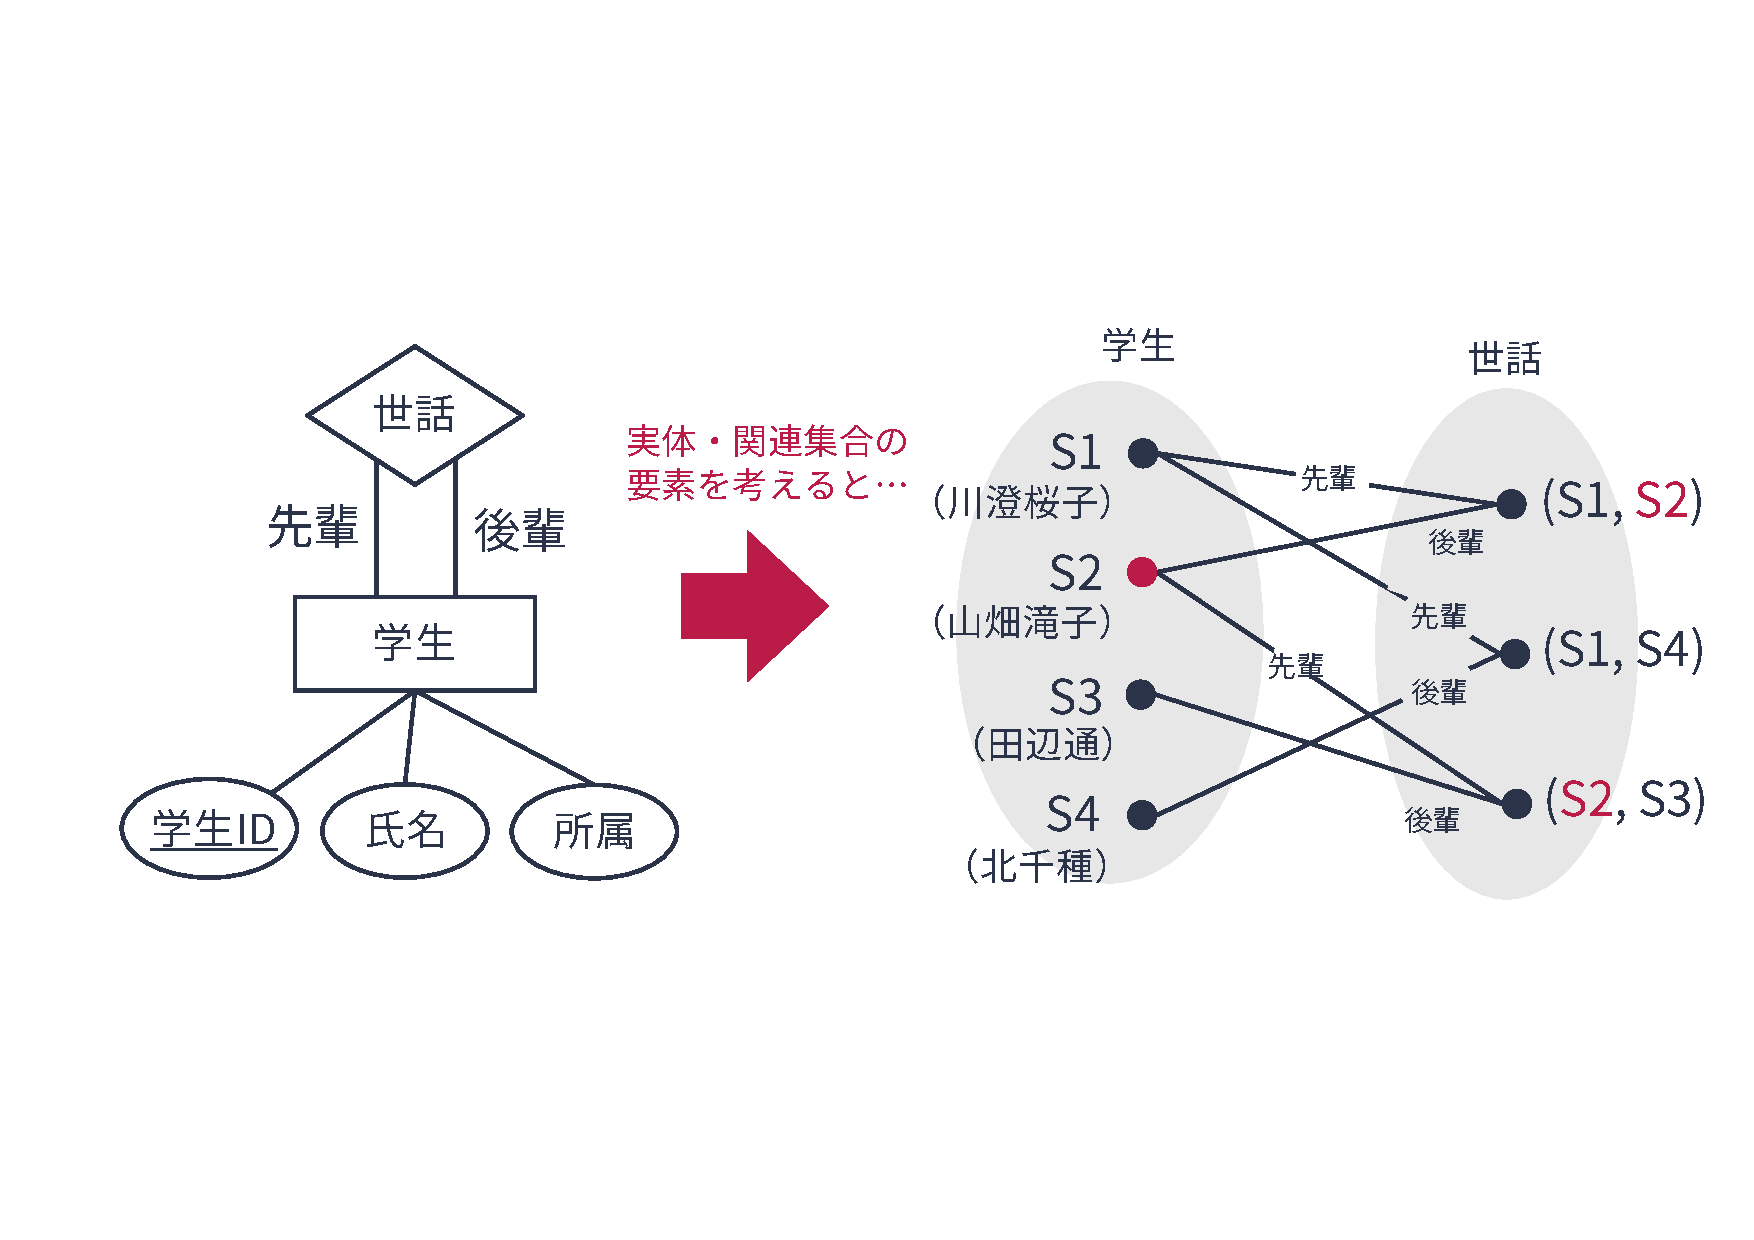
\includegraphics[width=1.0\textwidth]{figure/er-model/er-model-with-role.pdf}
    \caption{役割を明示した実体関連図の例}
    \label{fig:er_model_with_role}
\end{figure}


\begin{notebox}{実体，関連，属性を見分ける経験則}
与えられたシナリオから実体関連図を作成しようとしても，何を実体として何を関連として見なすか，どれを属性として見なすか，迷うことがあるでしょう．
実体関連モデルを提唱したPeter Chenは自身が発表した論文\cite{Chen1997}において，以下のような経験則を提案しています．
\begin{itemize}
\item 普通名詞: 実体型
\item 固有名詞: 実体
\item 他動詞: 関連型
\item 自動詞: 属性
\item 形容詞: 実体の属性
\item 副詞: 関連の属性
\end{itemize}
以上の経験則は当てはまらないこともありますが，一定の目安にはなります．
実体関連モデルを習い始めたばかりの人は参考にしてみてください．
\end{notebox}


\section{実体関連モデルにおける一貫性制約}
関係データモデルでは，対象となるデータが持つべき条件としてドメイン制約やキー制約といった一貫性制約を定義します．
実体関連モデルにおいても，データが持つべき一貫性制約を表現・設定する方法がいくつか用意されています．
以下では，実体関連モデルにおける代表的な一貫性制約である\strong{参加制約}，\strong{多重度制約}，\strong{キー制約}について説明します．

\subsection{参加制約}
図\ref{fig:er_model_elements2}を見てみましょう．
図\ref{fig:er_model_elements2}は，あるショッピングサイトにおける商品の「お気に入り」に関する実体型および関連型の要素を示したものです（図\ref{fig:er_model_elements}と似ていますが，問題のあった関連（お気に入り\graybox{(U1,P1)}の2つ目）を取り除き，商品\graybox{P3}を追加しています）．
図の実体型「商品」に注目すると，どの実体「ユーザ」とも関連を持たない実体「商品」\graybox{タケノコの里（P3）}が存在していることが分かります．
これは，誰も商品\graybox{P3}の購入を希望していないことを意味します．
\figure[htb]
    \centering
    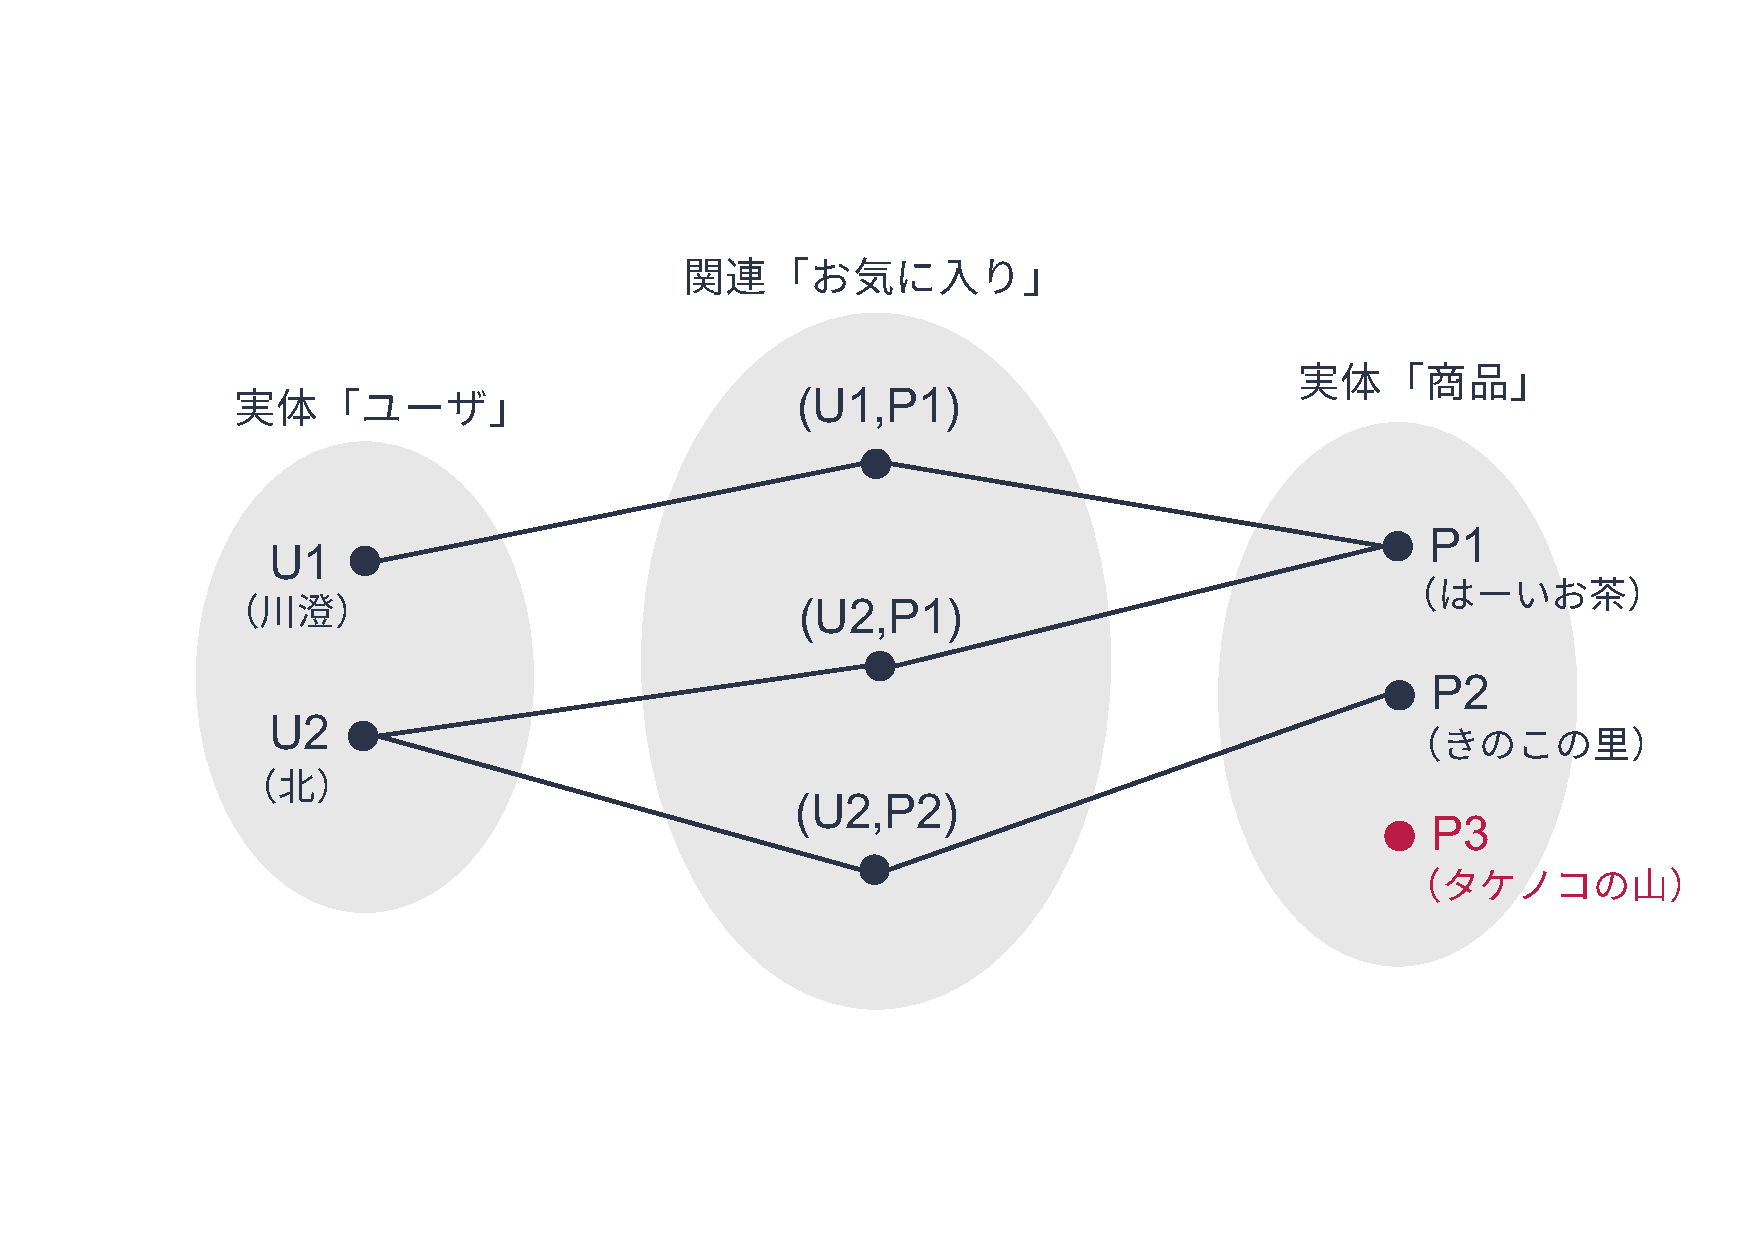
\includegraphics[width=0.85\textwidth]{figure/er-model/er-model-elements2.pdf}
    \caption{どの実体「ユーザ」とも関連を持たない実体「商品」が存在している例．}
    \label{fig:er_model_elements2}
\endfigure

実体関連図上で実体型$E_1$と実体型$E_2$が関連型$R$でつながっているときに，モデリングの対象としている問題設定によっては，実体集合$E_1$のすべての要素が関連集合$R$の要素とつながっていてほしい場合があります．
このようなケースを，$E_1$の$R$への参加は\strong{全体的}であると呼びます．

逆に$E_1$の集合内の全要素が関連集合$R$の全要素とつながっている必要がない場合，$E_1$の$R$への参加は\strong{部分的}であると呼びます．
実体型$E$の関連型$R$への参加が「部分的」であるときは，実体関連図上では$E$と$R$の間の直線を\strong{細線}にすることによって表現します．
例えば，先のショッピングサイトの図\ref{fig:er_model_elements2}のケースの場合，誰もお気に入りをしていない商品が存在しても構わないため，実体型「商品」は関連型「お気に入り」への参加は「部分的」としています．
このように，ある実体型のある関連型への参加（つながり）が全体的か部分的かを定める制約を\strong{参加制約（participation constraint）}と呼びます．

実体型$E$の関連型$R$への参加が「全体的」であるとき，実体関連図上では$E$と$R$の間の直線を\strong{太線}にすることによって表現します．
例えば，先のショッピングサイトの例において，実体型「商品」の関連型「お気に入り」への参加が「全体的」であるとするときは，図\ref{fig:participation_constraint}のような実体関連図にします．
\figure[tb]
    \centering
    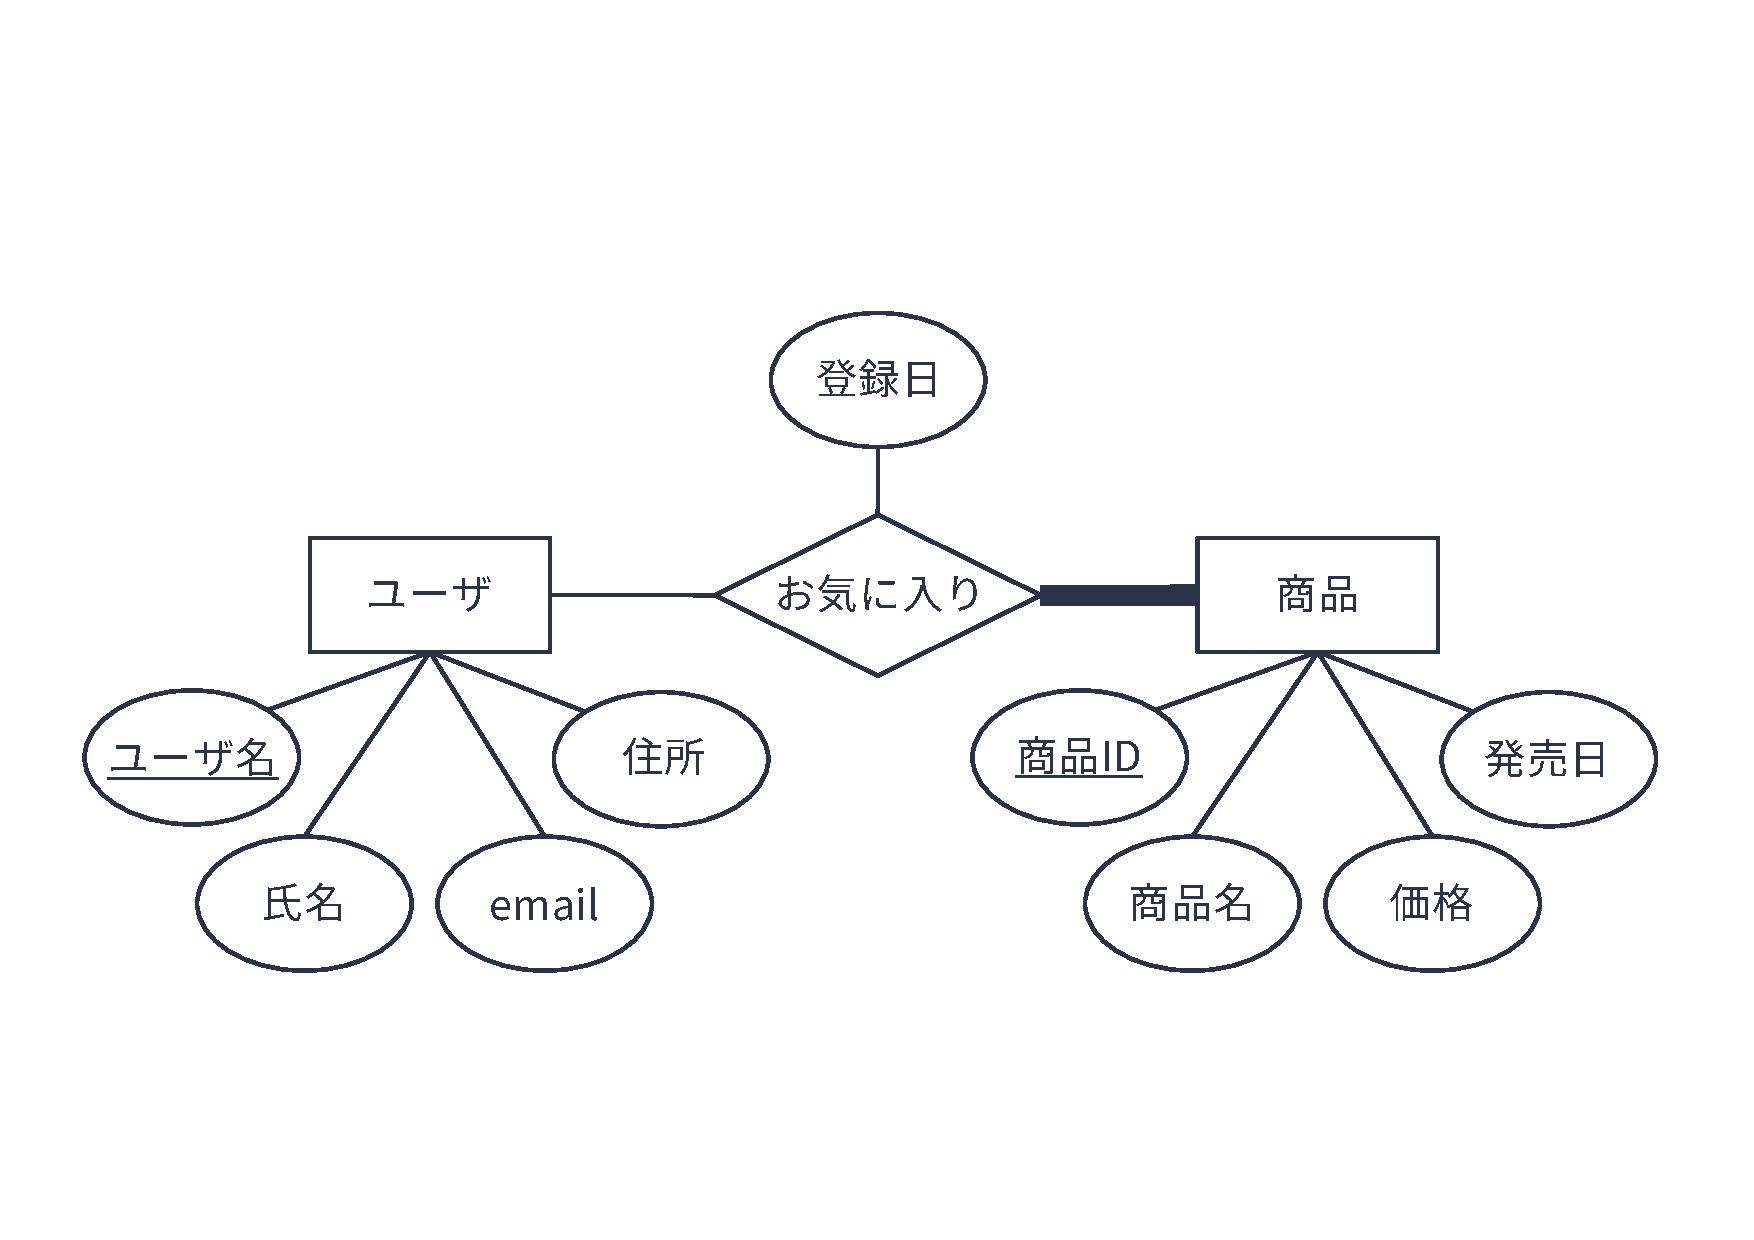
\includegraphics[width=1.0\textwidth]{figure/er-model/participation-constraint.pdf}
    \caption{参加制約の例}
    \label{fig:participation_constraint}
\endfigure
図\ref{fig:participation_constraint}のように定義することで，どの実体「商品」も必ずいずれかの関連「お気に入り」とつながっている必要があります．
逆に，図では実体「ユーザ」は関連「お気に入り」への参加が「部分的」となっているため，つまりお気に入り登録したことがないユーザが存在することを許しているということにもなります．


\subsection{多重度制約}
ショッピングサイトの例に戻りましょう．
図\ref{fig:er_model_elements3}は，お気に入り登録に加えて，各商品がどのメーカーによって製造されたかの情報についても管理する実体関連モデルを設計し，それに基づき実体集合「ユーザ」「商品」「メーカー」および関連集合「お気に入り」「製造」の要素を図示したものです．
\figure[htb]
    \centering
    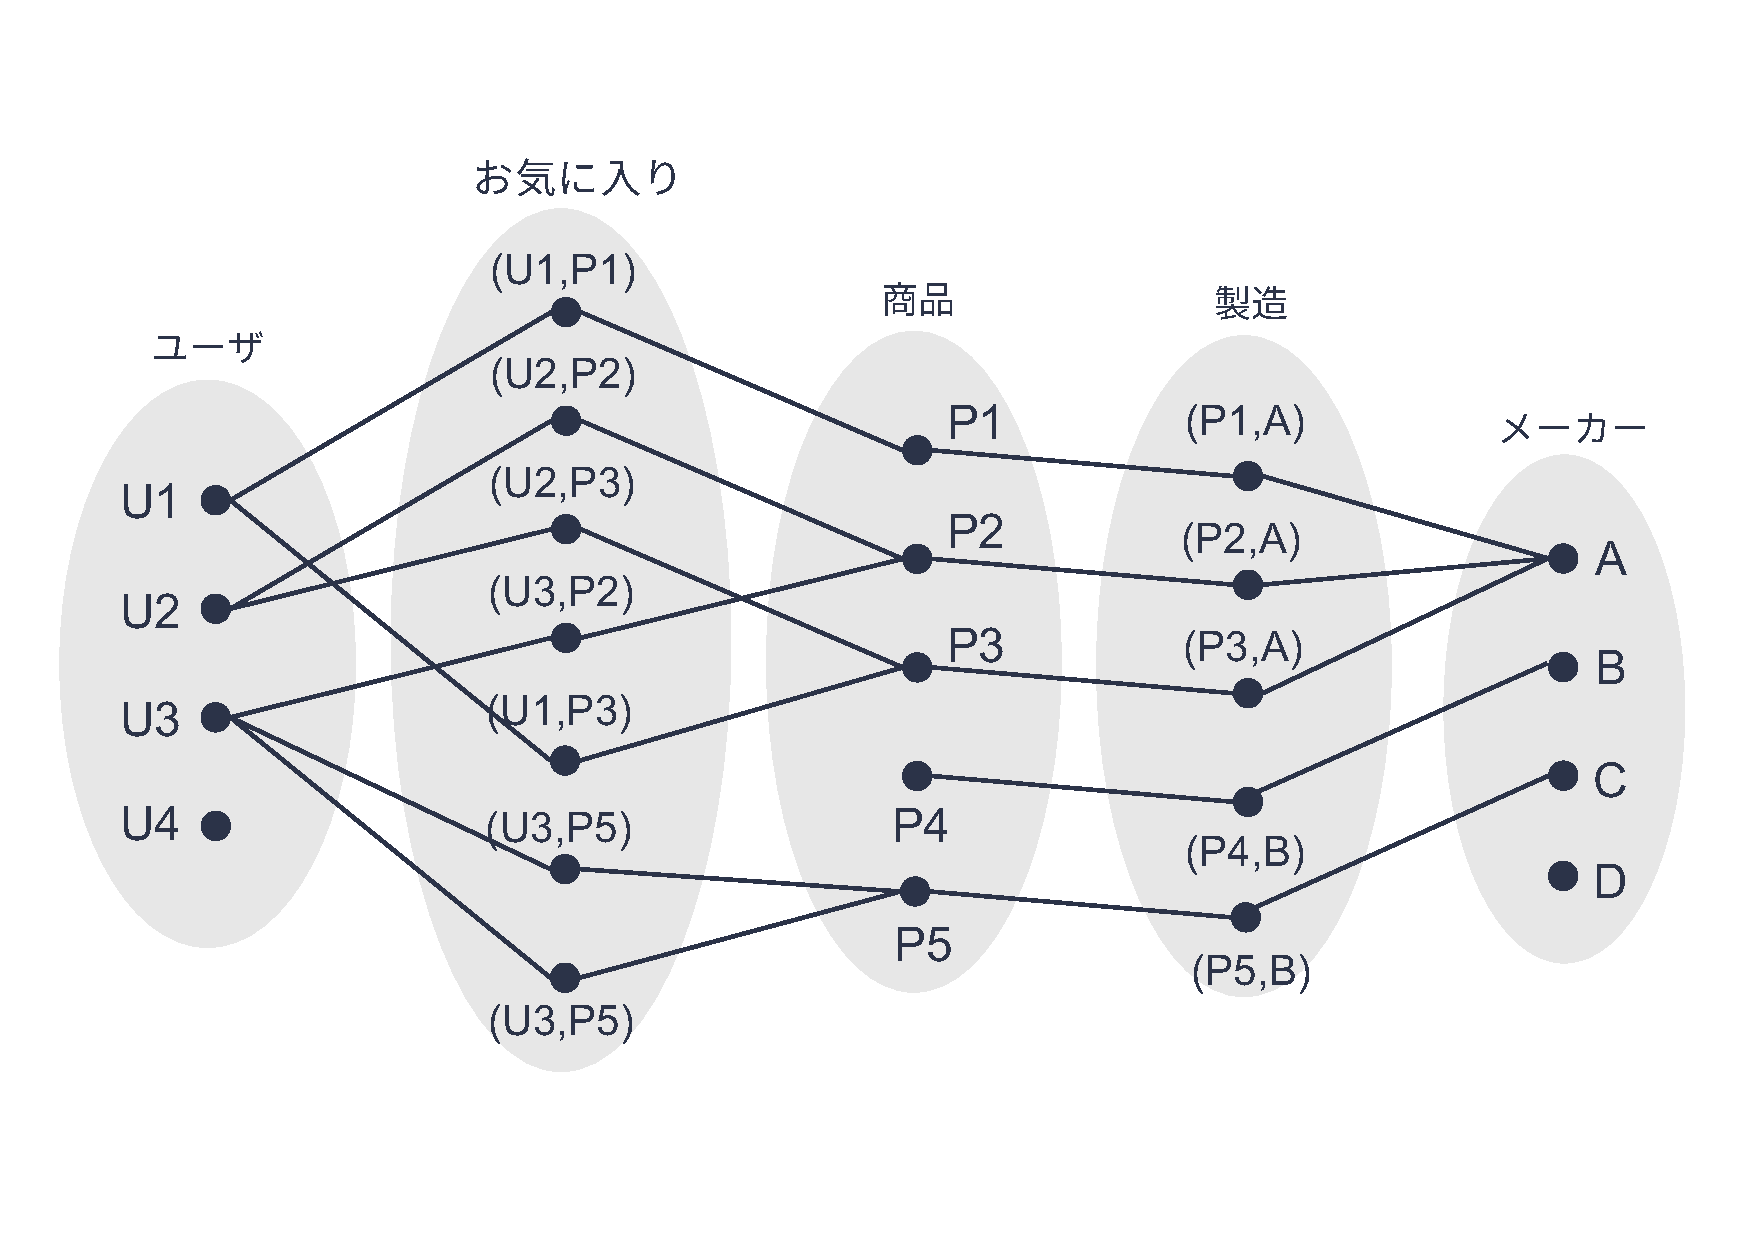
\includegraphics[width=1.0\textwidth]{figure/er-model/er-model-elements3.pdf}
    \caption{実体「メーカー」と関連「製造」も加えた実体関連図の要素の例．}
    \label{fig:er_model_elements3}
\endfigure
（図が物語っていることがすべてであるとすると）この図からは，以下のことが分かります．
\begin{enumerate}
\item ユーザは複数の商品をお気に入り登録することができる
\item 商品は複数のユーザからお気に入り登録されてもよい
\item ユーザの中には商品をお気に入り登録をしない者がいてもよい
\item 商品の中にはユーザにお気に入り登録されないものがあってもよい
\item 商品は必ず1つのメーカーによって製造される（複数のメーカーが合同で1つの商品を製造することはない）
\item メーカーは複数の商品を製造する
\item メーカーの中には商品を製造していないところがあってもよい
\end{enumerate}

以上のことを実体関連図上で表現してみましょう．
上記項目のうち，項目3，4，5，7については参加制約に関する事柄です．
すなわち，
\begin{itemize}
\item 実体型「ユーザ」の関連型「お気に入り」への参加制約は「部分的」
\item 実体型「商品」の関連型「お気に入り」への参加制約は「部分的」
\item 実体型「商品」の関連型「製造」への参加制約は「全体的」
\item 実体型「メーカー」の関連型「製造」への参加制約は「部分的」
\end{itemize}
となります．

一方，項目1，2，6（そして5）は，ある実体（要素）から見たときに，ある関連を通じて異なる実体（要素）と「いくつ」つながることが許されるかという制約を示しています．
このように，ある関連に対して対応づけ可能な実体の数を\strong{多重度（cardinality）}\footnote{Cardinalityは多重度と呼ばれることもあるが，語源からすると「濃度」が正しい訳語とする説がある．}と呼びます．
また，多重度に関する制約を\strong{多重度制約（cardinality constraint）}と呼びます．

実体間の関連は「1対1」「1対多」「多対多」のいずれかとなります．
例えば，上記図においては
\begin{itemize}
\item 関連「お気に入り」はユーザと商品の「多対多」関連（項目1および2）
\item 関連「製造」はメーカーと商品の「1対多」関連（項目5および6）
\end{itemize}
と見なせます．

実体関連図において，多重度は以下のように表現します．
\begin{itemize}
\item 1対1関連: 関連型から実体型に引かれた線をすべて矢印線にする
\item 1対多関連: 関連型から「1」に対応する実体型に引かれた線のみを矢印線にする
\item 多対多関連: 関連型から実体型に引かれた線をすべて直線にする（矢印は加えず，そのままにする）
\end{itemize}
図\ref{fig:er_model_elements3}の内容を踏まえて実体関連図を設計すると，図\ref{fig:cardinality_constraint}のようになります．
例えば，関連型「お気に入り」から実体型「ユーザ」への線は直線に，関連型「製造」から実体型「メーカー」への線は矢印線になります．
\begin{figure}[htb]
    \centering
    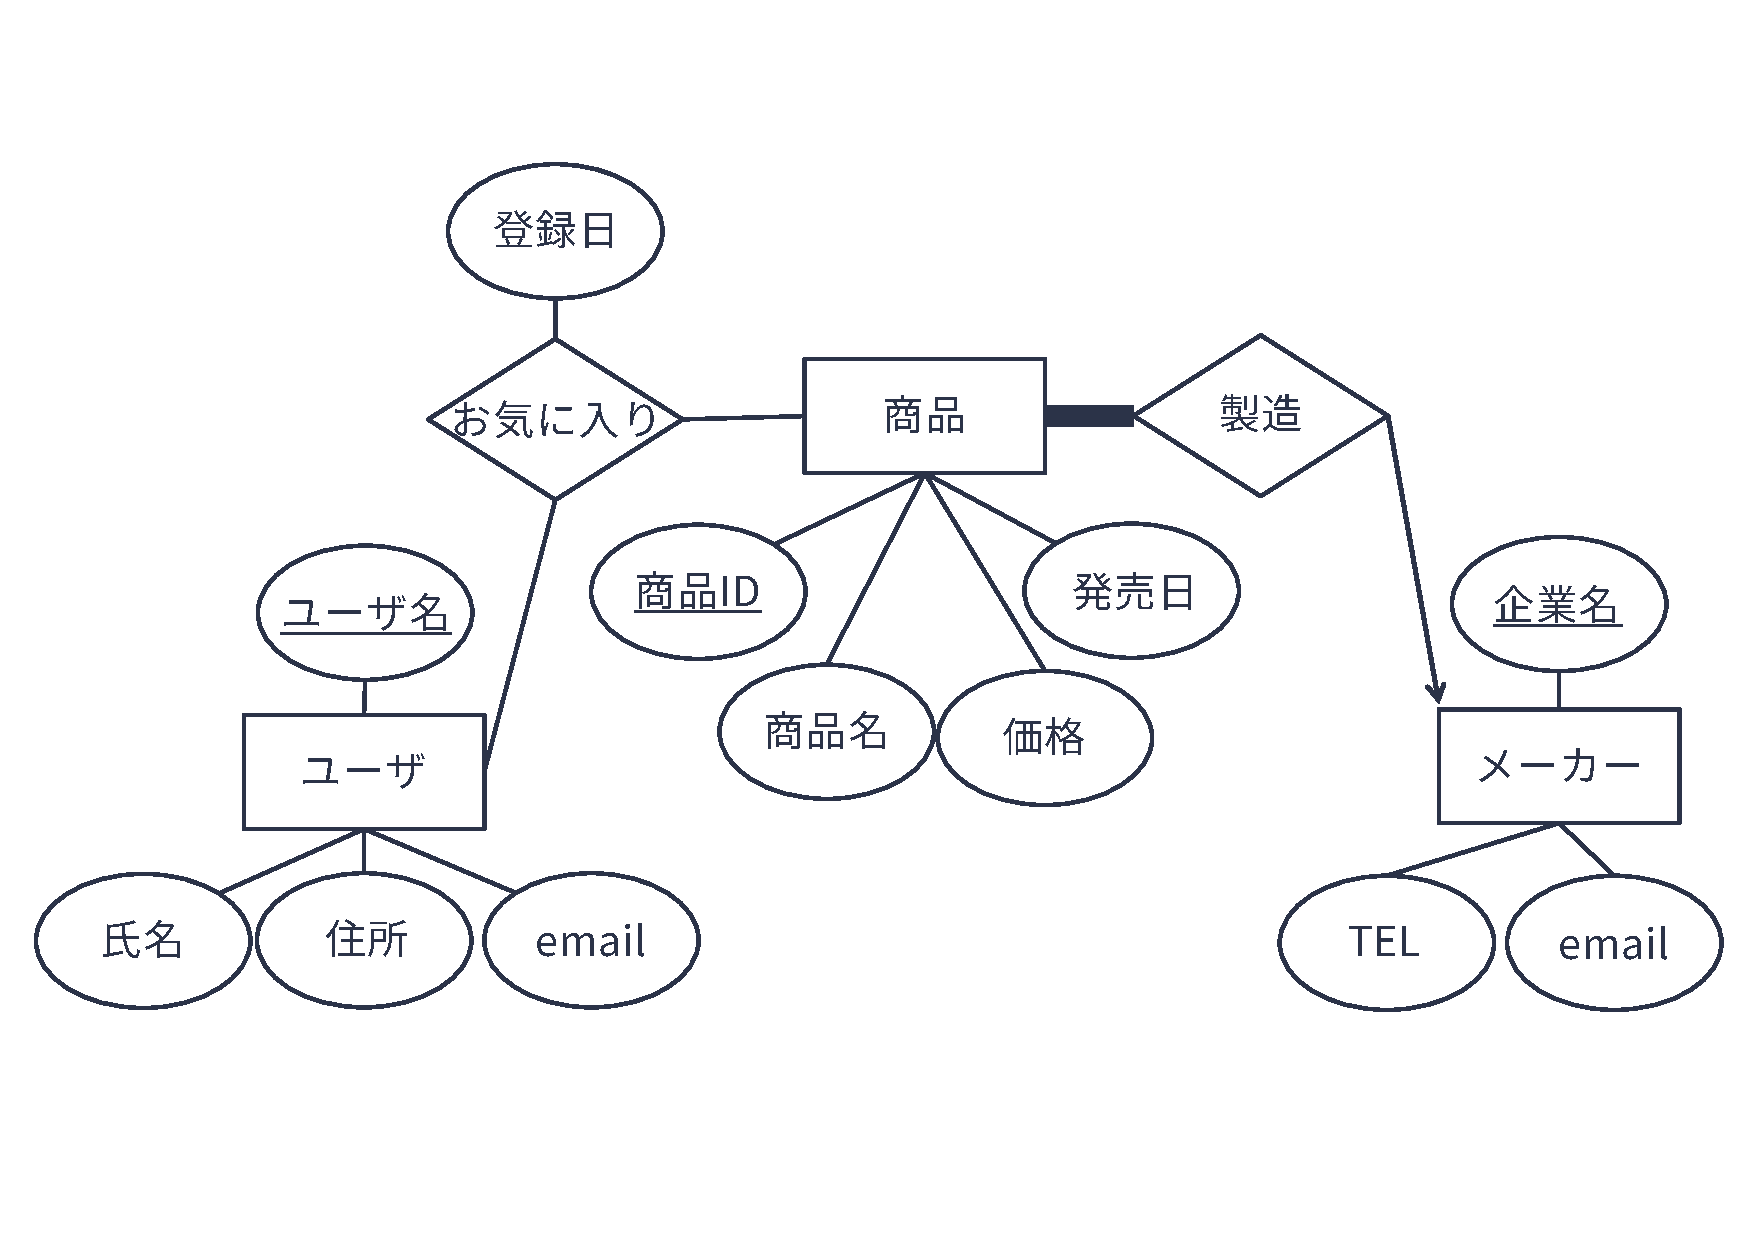
\includegraphics[width=1.0\textwidth]{figure/er-model/cardinality-constraint.pdf}
    \caption{多重度制約を表現した実体関連図の例．}
    \label{fig:cardinality_constraint}
\end{figure}


\subsection{キー制約}
実体関連モデルにおける\strong{キー制約（key constraint）}とは，キーとして指定された属性はキーとしての役割を必ず果たす必要があるという制約です．
例えば，実体型「学生」の属性「学籍番号」が主キーとして設定された場合，指定された学籍番号によって実体「学生」は一意に特定できなければなりません．
また，学籍番号に重複は許されません．
実体型の説明で述べたように，実体関連図において主キーとなる属性には下線を引きます．

\subsubsection{弱実体と部分キー}
ショッピングサイトの例に戻りましょう．
ショッピングサイトを利用する際，自分のユーザ名を使ってログインをしたものの，購入した商品の送り先を同居する家族の名前にしたい，というケースを考えましょう．
このようなケースに対応するため，サイト運営者は先ほど示した図\ref{fig:cardinality_constraint}の実体関連図を改善して，
\begin{itemize}
\item 実体型「家族」を追加
\item 実体「ユーザ」と実体「家族」が同居関係にあることを示すために，関連型「同居」を追加
\end{itemize}
すること検討しているとしましょう．
この際，「家族」にはユーザ名は割り振られず，家族の誰かに商品を送るときは，その家族のユーザがサイトにログインをして手続きをすることを想定してください．

このようなケースは，\strong{弱実体}という特殊な概念を用いて実体関連図を設計することがあります．
自身がもつ属性だけでは主キーを構成できない特殊な実体集合を\strong{弱実体集合（weak entity set）}と呼びます．
弱実体を特定する上で，それと関連している実体のことを\strong{所有実体（owner entity）}と呼びます．
弱実体と所有実体をつなげる関連を\strong{弱関連（weak relationship）}と呼びます．
また，弱実体を一意に特定するために，所有実体の主キーとセットにして使われる弱実体の属性を\strong{部分キー（partial key）}と呼びます．
所有実体と部分キーが決まって初めて，弱実体集合の中にある弱実体を一意に特定できるようになります．

実体関連図において，弱実体型は二重線の矩形，弱関連型は二重線のひし形で表現します．
また，部分キーには点線を引きます\footnote{書籍によっては部分キーには下線を引くと書かれている場合もありますが，本書では主キーと分かりやすく区別するために点線を用います}．

先の家族を扱うケースについて，弱実体と弱関連の概念を用いても実体関連図を作成すると，図\ref{fig:weak_entity}のようになります．
図\ref{fig:weak_entity}においては，
\begin{itemize}
\item 実体「家族」が弱実体（「氏名」が部分キー）
\item 実体「ユーザ」が（弱実体「家族」に対する）所有実体
\item 関連「同居」が弱関連
\end{itemize}
となります．
図中では，弱実体型「家族」は「氏名」「続柄」のみを属性として持っています．
なお，「氏名」は部分キーであり，弱実体型「家族」の主キーに設定していません．
主たるユーザがいてこその弱実体「家族」であり，「家族」を独立して管理する意味がないからです．
\begin{figure}[tb]
    \centering
    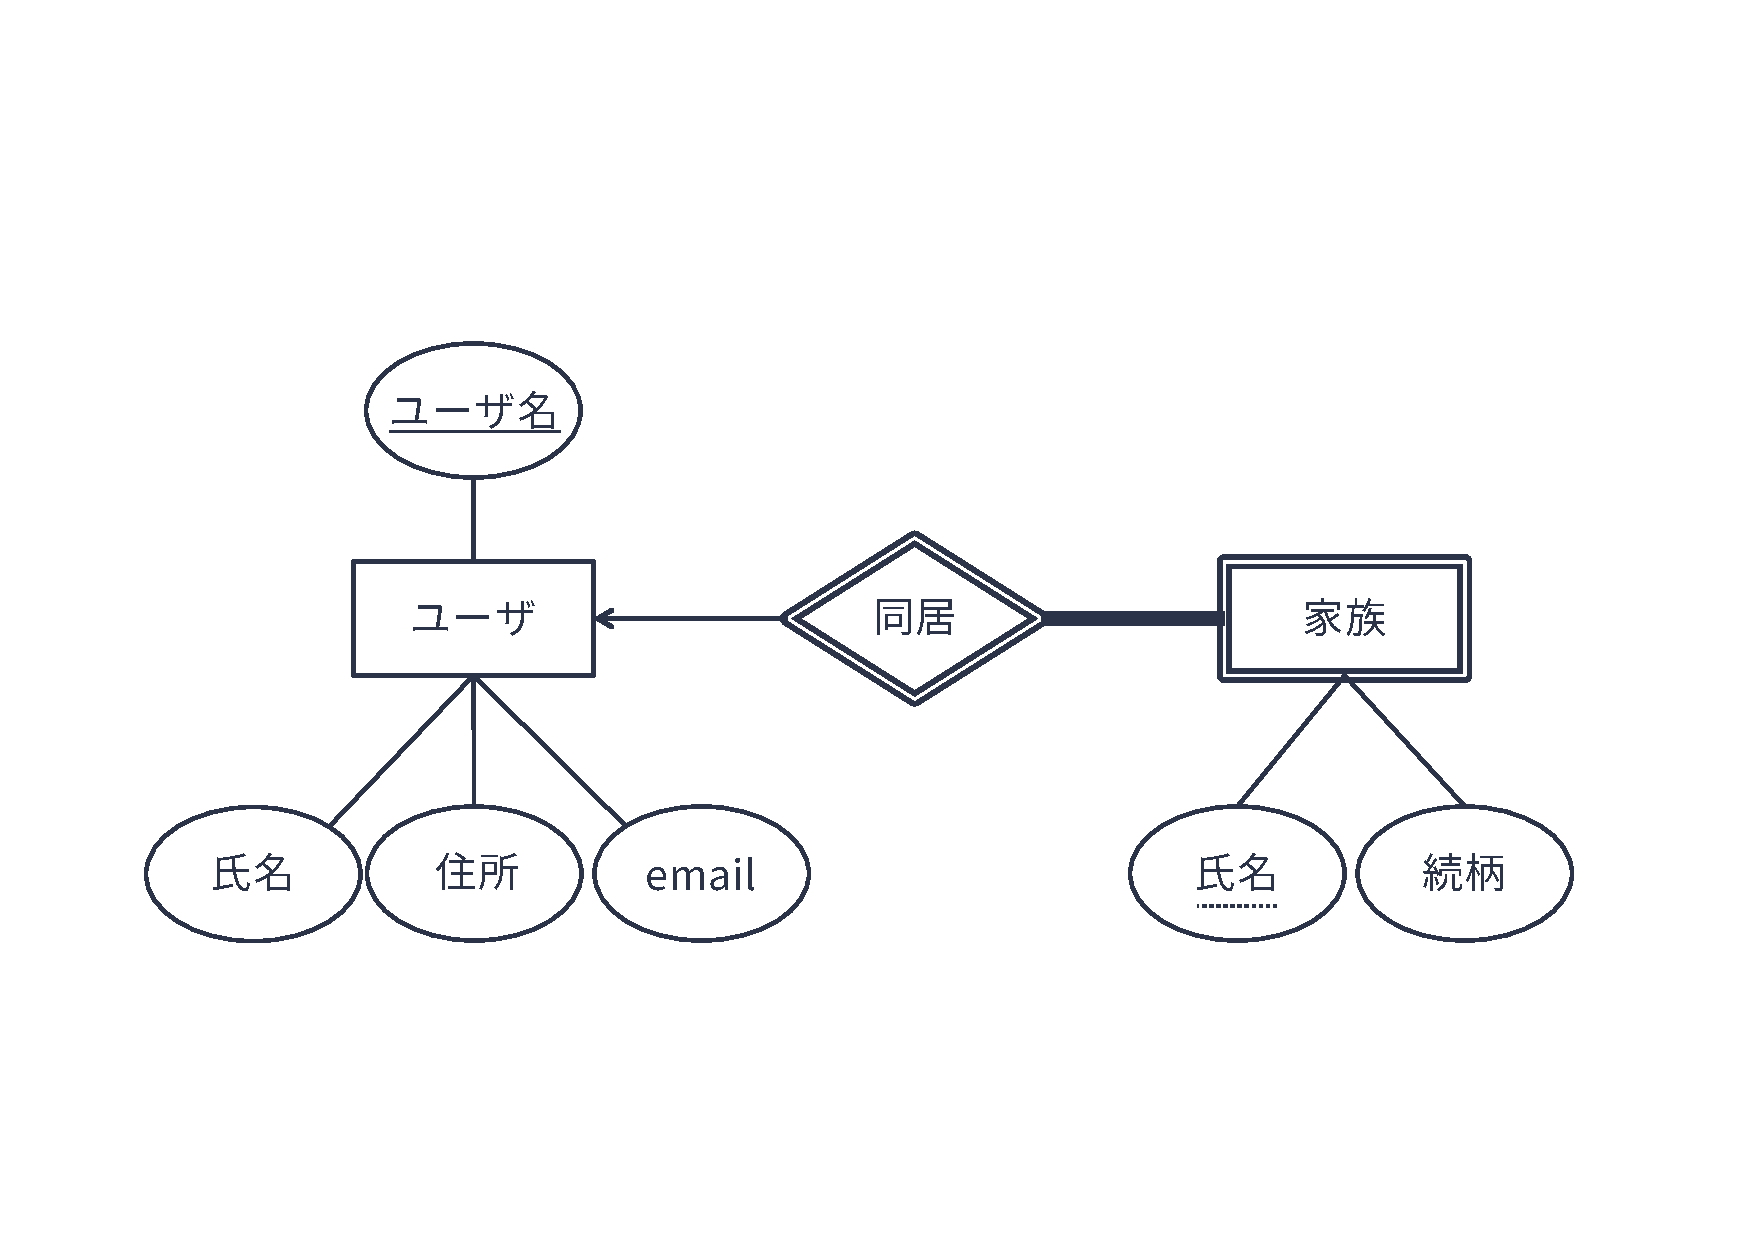
\includegraphics[width=1.0\textwidth]{figure/er-model/weak-entity.pdf}
    \caption{弱実体の例}
    \label{fig:weak_entity}
\end{figure}

図\ref{fig:weak_entity}の実体関連図を設計をすると，あるユーザを特定した際，そのユーザに関連「同居」で紐付いている実体「家族」については「氏名」によって特定が可能となります．
言い換えると，実体「ユーザ」の情報なしに「氏名」だけですべての弱実体集合「家族」に存在する，条件を満たす弱実体「家族」を特定することはできません．
これは，弱実体「家族」は自身がもつ属性だけでは主キーを構成できないことを意味します．


\begin{notebox}{弱実体はなぜ「弱」いのか？}
図\ref{fig:weak_entity}の実体関連図において，実体「家族」が弱実体としました．
読者によっては，実体「家族」にも主キーを持たせて，所有実体「ユーザ」の主キーがなくても一意に特定できるようにすればよいのでは，と考えた方がいるかもしれません．
そのようにすることも理論的にも運用上も可能です．
しかし，「家族」をあえて弱実体にしているのは，対象としているショッピングサイトの運用指針にも関係しています．

例に挙げたショッピングサイトにおいては，あくまでユーザIDをもつ「ユーザ」が販売活動の中心となっています．
あるユーザの「家族」に商品を送るというのは，その家族がユーザのIDを借りて商品を買っていると見なせます．
これは，ユーザIDを持つユーザが家族にいなければ，商品を送ってもらえない（買えない）ことを意味します．
つまり，弱実体「家族」は所有実体「ユーザ」が存在しなければ存在できない「弱い」存在であり，ある「ユーザ」が削除されるとそれと紐付いている「家族」も同時に抹消されてしまいます．

あえて「家族」を弱実体にすることは，データベースに対して「（アカウントを持つ）ユーザの存在なしにその家族の存在は認めない」というデータベース設計者の強い意図の表れと言えます．
\end{notebox}


\begin{tipbox}{弱実体にすべきか否か}
弱実体の概念は初学者には非常に難しいため，実体関連モデルの設計において弱実体を用いるべきか，迷うシーンが出てくると思います．
結論からいえば，弱実体を用いるべきかどうかは理論的に正解があるわけではなく，データベース上で対象をどう定義し，扱いたいかという設計方針によって決まります．

弱実体を用いるべきかの判断基準としては，いくつかのポイントがあります．
1つは，対象が主キーを持たせることができそうか，関連する（所有）実体の存在なしに特定できるように設計できそうかという点です．
例えば，図書館における図書の管理について考えてみましょう．
図書館は同じ書籍を複数冊所蔵して，それらを図書として貸し出せるようにしていることが多いです．
このようなケースでは，「図書」のキーを「書籍」のISBN番号と連番の組みあわせ（連番が部分キー）で表現すれば，「書籍」を所有実体，「図書」を弱実体として設計することができます．
一方，「図書」1冊1冊に図書ID（図書館専用のバーコード番号のようなもの）という一意に識別可能な値を割り振れば，理論上は「図書」を通常の実体として扱えます．
ISBN番号が何であろうと，図書館が保有しているある図書を特定できるからです．

2つ目のポイントは，運用上のメリットです．
1つ目のポイントで説明したように，ケースによっては通常の実体でも弱実体でもどちらでも設計することが可能なケースがあります．
弱実体ではなく通常の実体として扱った方が運用上のメリットがあるケースとしては，例えば，図書館の例ですと，ISBN番号が割り振られていない古い書籍を管理したい場合などが考えられます．

あえて弱実体を用いたほうが良さそうなケースとしては，弱実体として扱うべきか迷っている対象が\strong{所有実体の属性のような存在}である場合です．
例えば，先のショッピングサイトの例における「ユーザ」と「家族」の関係であったり，ショッピングサイトにおける「注文」とその「明細」の関係などが挙げられます．
どちらの例も，弱実体は所有実体の「属性」的な扱いであり，所有実体がなければ弱実体だけを管理する意味がないと考えられます．
\end{tipbox}


\section{汎化・継承}
素朴な実体関連モデルを拡張するアイデアが提案されています．
そのうちのひとつが，\strong{汎化・継承}の概念です\cite{Bancilhon1992}．

実世界を実体関連モデルで表現する際，実体集合間にある種の包含関係（階層関係）が想定される場合があります．
例えば，実体型「大学構成員」「学生」「教員」を考えてみましょう．
学生も教員も大学を構成するメンバーです．
そのため「大学構成員」と「学生」「教員」は包含関係にあると見なせます．

今，ある大学のデータ管理者は，大学構成員の情報を管理する上で，
\begin{itemize}
\item 学生には「大学ID」「氏名」「生年月日」「性別」「所属」と「入学年」
\item 教員には「大学ID」「氏名」「生年月日」「性別」「所属」と「研究者ID」「職階」
\end{itemize}
の情報を持たせたいと考えているとしましょう．
実体関連モデルで実体型「学生」「教員」を定義するには，どうしたらよいでしょうか．

ここで，あらかじめ「大学ID」「氏名」「生年月日」「性別」「所属」を属性とする実体型「大学構成員」が定義されているとしましょう．
このとき，
\begin{quotation}
実体型「学生」は属性「大学ID」「氏名」「生年月日」「性別」「所属」「入学年」を持つ実体型である
\end{quotation}
と定義するよりも，
\begin{quotation}
実体型「学生」は実体型「大学構成員」に属性「入学年」を加えた実体型である
\end{quotation}
と定義したほうが無駄が少ないですし，自然でもあります．
実体型「教員」の定義においても同様のことが言えます．
このように定義しておけば，仮に実体型「学生」と「教員」のそれぞれに「メールアドレス」という属性を持たせたいときも，実体型「大学構成員」に「メールアドレス」という属性を加えるだけで済みます．

このように，実体型$E_1$が持つすべての属性を持つと考え，新たな実体型$E_2$を定義するとき，$E_2$は$E_1$を\strong{継承（inherit）}したといいます（「$E_1$は$E2$を\strong{汎化（generalize）}した実体型である」と称することもあります）．
継承を用いて実体型を表現したとき，その実体集合（下位の集合）は継承元（上位）の実体集合にすべて包含されることになります．

実体関連図において，継承元となる上位の実体型と継承先となる下位の実体型の間には，汎化・継承関係があることを示す「isa」と記した三角の特別な関連記号を置きます．
例えば，先の実体型「大学構成員」「学生」「教員」を汎化・継承の概念を使って実体関連図を書くと，図\ref{fig:inheritance}のように表現できます．
\figure[tb]
    \centering
    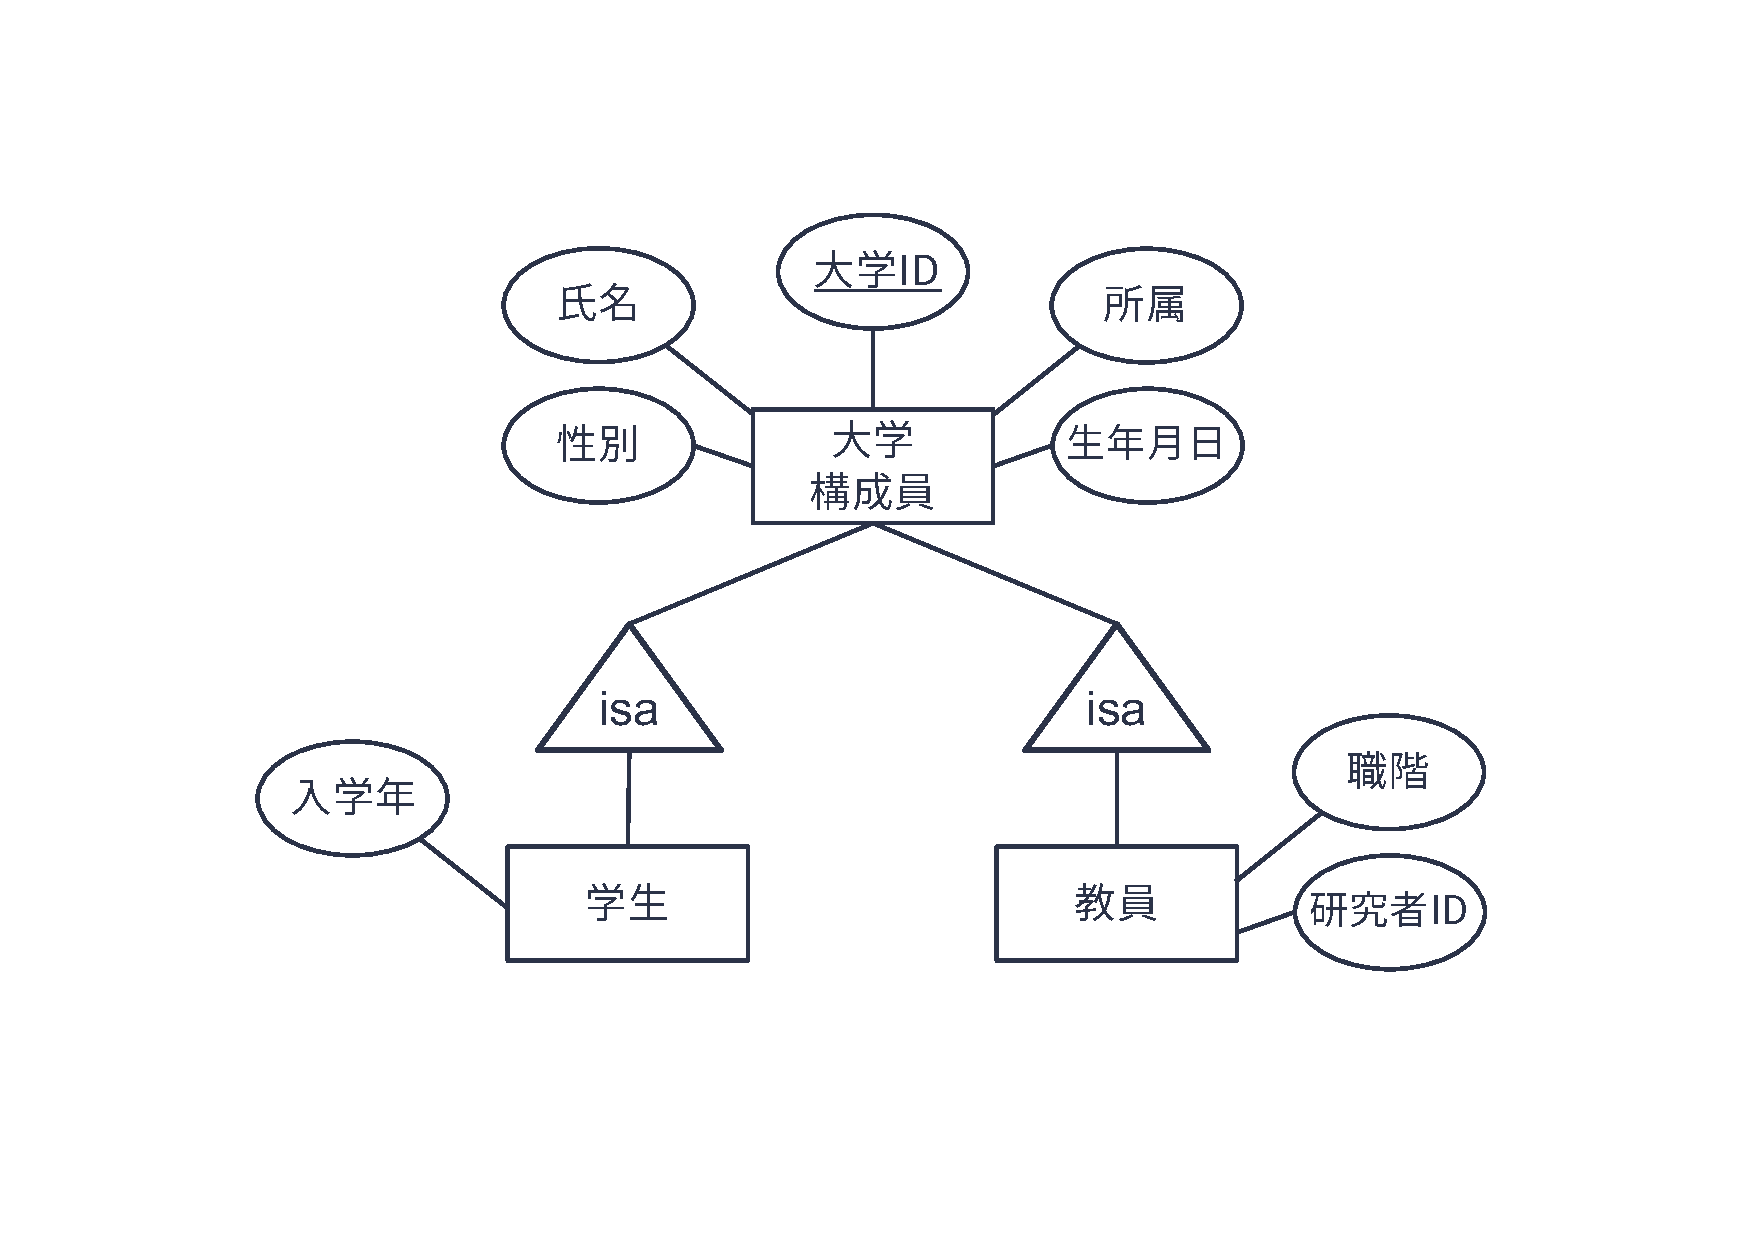
\includegraphics[width=0.8\textwidth]{figure/er-model/inheritance.pdf}
    \caption{汎化・継承の例}
    \label{fig:inheritance}
\endfigure


\section{n項関連}
これまでの説明で扱ってきた関連型は，2つの実体型とのつながりを表現したもの（2項関連）に限定されていましたが，3つ以上の実体型とつながりがあっても問題ありません．
むしろ，現実世界の状況を表現するために，3つ以上の実体型をつなぐ関連が必要になることがしばしばあります．
n個の実体型をつなぐ関連を\strong{n項関連（n-ary relationship）}と呼びます．
2項関連と同様に，n項関連においても参加制約や多重度制約を考えることができます．

\figure[htb]
    \centering
    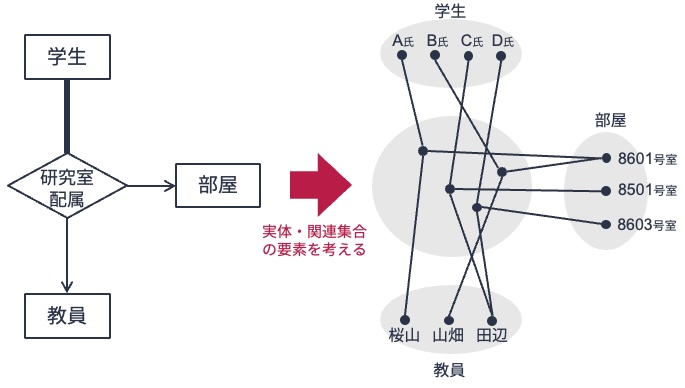
\includegraphics[width=1.0\textwidth]{figure/er-model/3-ary-relationship1.jpg}
    \caption{3項関連の例}
    \label{fig:3-aryrelationship1}
\endfigure
図\ref{fig:3-aryrelationship1}は，学生がどこの教室でどの教員の指導をうけるかを実体関連図で表現した図（左）および各実体集合，関連集合の要素を示した図（右）です．
図\ref{fig:3-aryrelationship1}では，関連型「研究室配属」は実体型「学生」「部屋」「教員」の3項関連となっています．
また，図中の実体関連図が示しているように，関連型「研究室配属」において，
\begin{itemize}
\item 「学生」と「教員」は多対1の関連
\item 「学生」と「部屋」は多対1の関連
\end{itemize}
となっています．
これは，学生の指導教員は必ず1名であり，学生に割り当てられる部屋割も必ず1つに決まる，ということを意味します．．

\figure[htb]
    \centering
    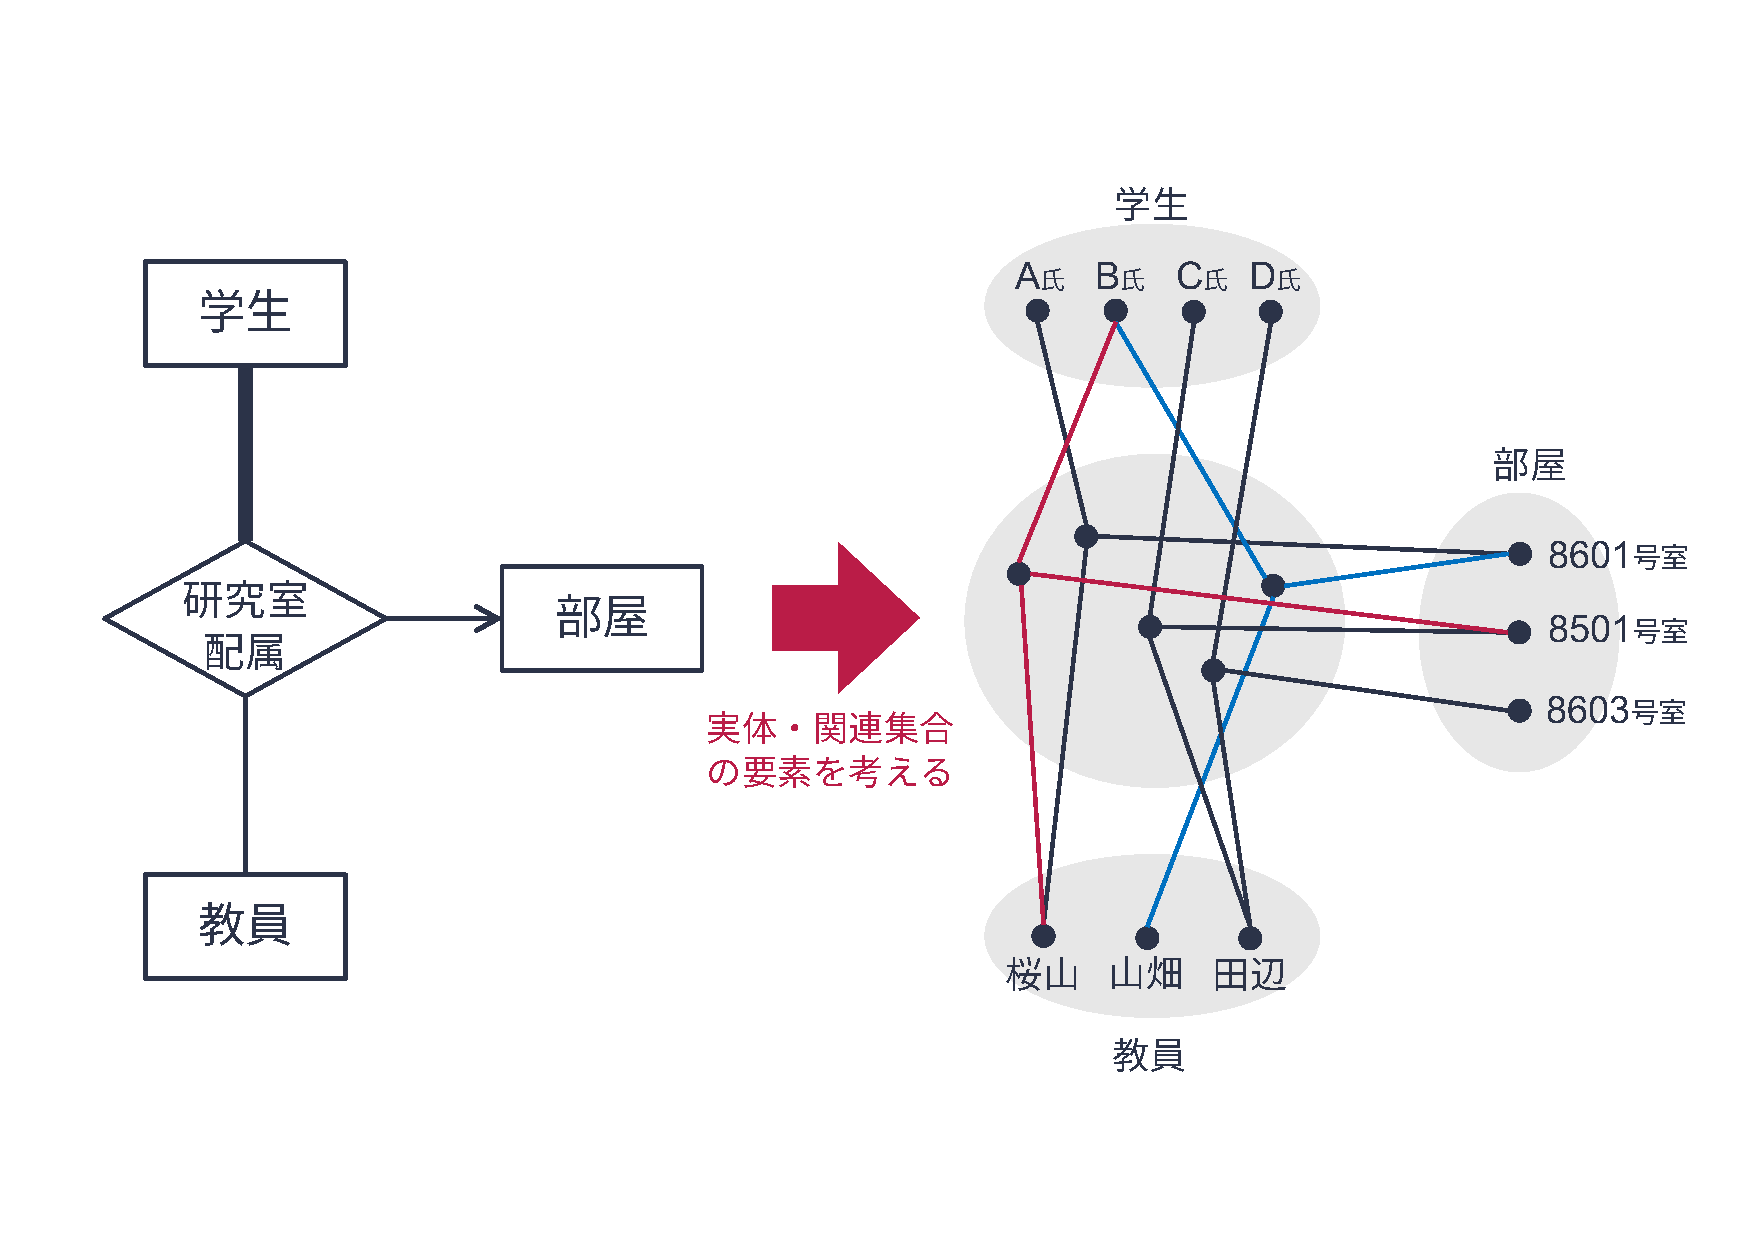
\includegraphics[width=1.0\textwidth]{figure/er-model/3-ary-relationship2.pdf}
    \caption{3項関連の例2}
    \label{fig:3-ary-relationship2}
\endfigure
一方，図\ref{fig:3-ary-relationship2}は，先ほど同様，学生がどこの教室でどの教員の指導をうけるかを表した実体関連図および各実体集合，関連集合の要素を示した図ではありますが，実体関連図で表現されている内容が微妙に異なります．
図\ref{fig:3-ary-relationship2}の実体関連図においては，
\begin{itemize}
\item 「学生」と「教員」は多対多の関連
\item 「学生」と「部屋」は多対1の関連
\end{itemize}
となっていますが，解釈には注意が必要です．
n項関連においては，ある実体集合$E$に向かう矢印は，「関連する他のすべての実体集合から実体を1つずつ選んだとき，$E$の実体が1つに決まる」を意味すると定義されています．
これを踏まえると，図\ref{fig:3-ary-relationship2}においては，\strong{学生と教員の組みあわせ}に対応して部屋が1つに決まる，ということを意味します．
2項関係のように
\begin{itemize}
    \item 学生には複数の教員を割り当てることができる
    \item 学生に割り当てられる部屋は必ず1つである
\end{itemize}
と解釈してはいけません．
この実体関連図に対応する要素に関する図（図\ref{fig:3-ary-relationship2}の右図）を見ると，学生Bには桜山先生と山畑先生の2名の教員が指導教員として割り当てられていますが，部屋割は学生と教員の組みあわせに対して行われるため，学生Bは8501号室と8601号室の2部屋が割り当てられていることが分かります．


\section{実体関連モデルから関係スキーマへの変換}
本書で実体関連モデルを学ぶ理由は，実体関連モデルを関係データベースの設計に活用するためでした．
学習の締めくくりとして，実体関連モデルを関係スキーマに変換する方法を説明します．

実体関連モデルは概念モデルであり，そのままでは関係データベースシステム上で扱うことはできません．
そのため，論理モデルである関係データモデルに変換する必要があります．
この作業はそれほど難しいものではありません．
前節までに学習した実体関連図を用いれば，関係データモデルの構造を示す関係スキーマを\strong{機械的に}導出することができます．

以下，実体関連図のパターンに応じた関係スキーマへの変換方法を説明します．
説明には，実体関連モデルの解説で用いたオンラインショッピングの例を用います．

\subsection{変換パターン1：実体型}
実体型は
\begin{itemize}
\item 実体型名を関係スキーマの関係名
\item 実体型のキーを関係スキーマのキー
\item 実体型の属性を関係スキーマの属性
\end{itemize}
に対応させることで関係スキーマに変換できます．

図\ref{fig:erd-entity}に示した実体型「ユーザ」は以下のような関係スキーマに変換される
\begin{figure}[tb]
  \centering
  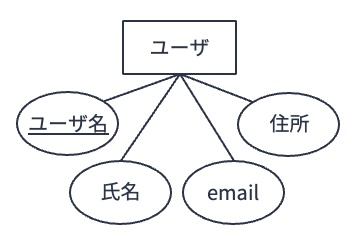
\includegraphics[width=0.6\textwidth]{figure/er-model/erd-entity.jpg}
  \caption{実体型「ユーザ」}
  \label{fig:erd-entity}
\end{figure}
\begin{equation}
  \text{ユーザ}(\underline{\text{ユーザ名}}, \text{氏名}, \text{住所}, \text{email})
\end{equation}


\subsection{変換パターン2：関連型}
関連型を関係スキーマに変換するには，基本的には
\begin{itemize}
\item 関連型名を関係スキーマの関係名
\item 関連型とつながる実体型のキーを関連型のキー
\item （あれば）関連型の属性を関係スキーマの属性
\end{itemize}
に対応させればよいです．
ただし，実体関連間の多重度によってキーの扱いが異なります．

\subsubsection{多重度が「多対多」の場合}
\begin{figure}[tb]
  \centering
  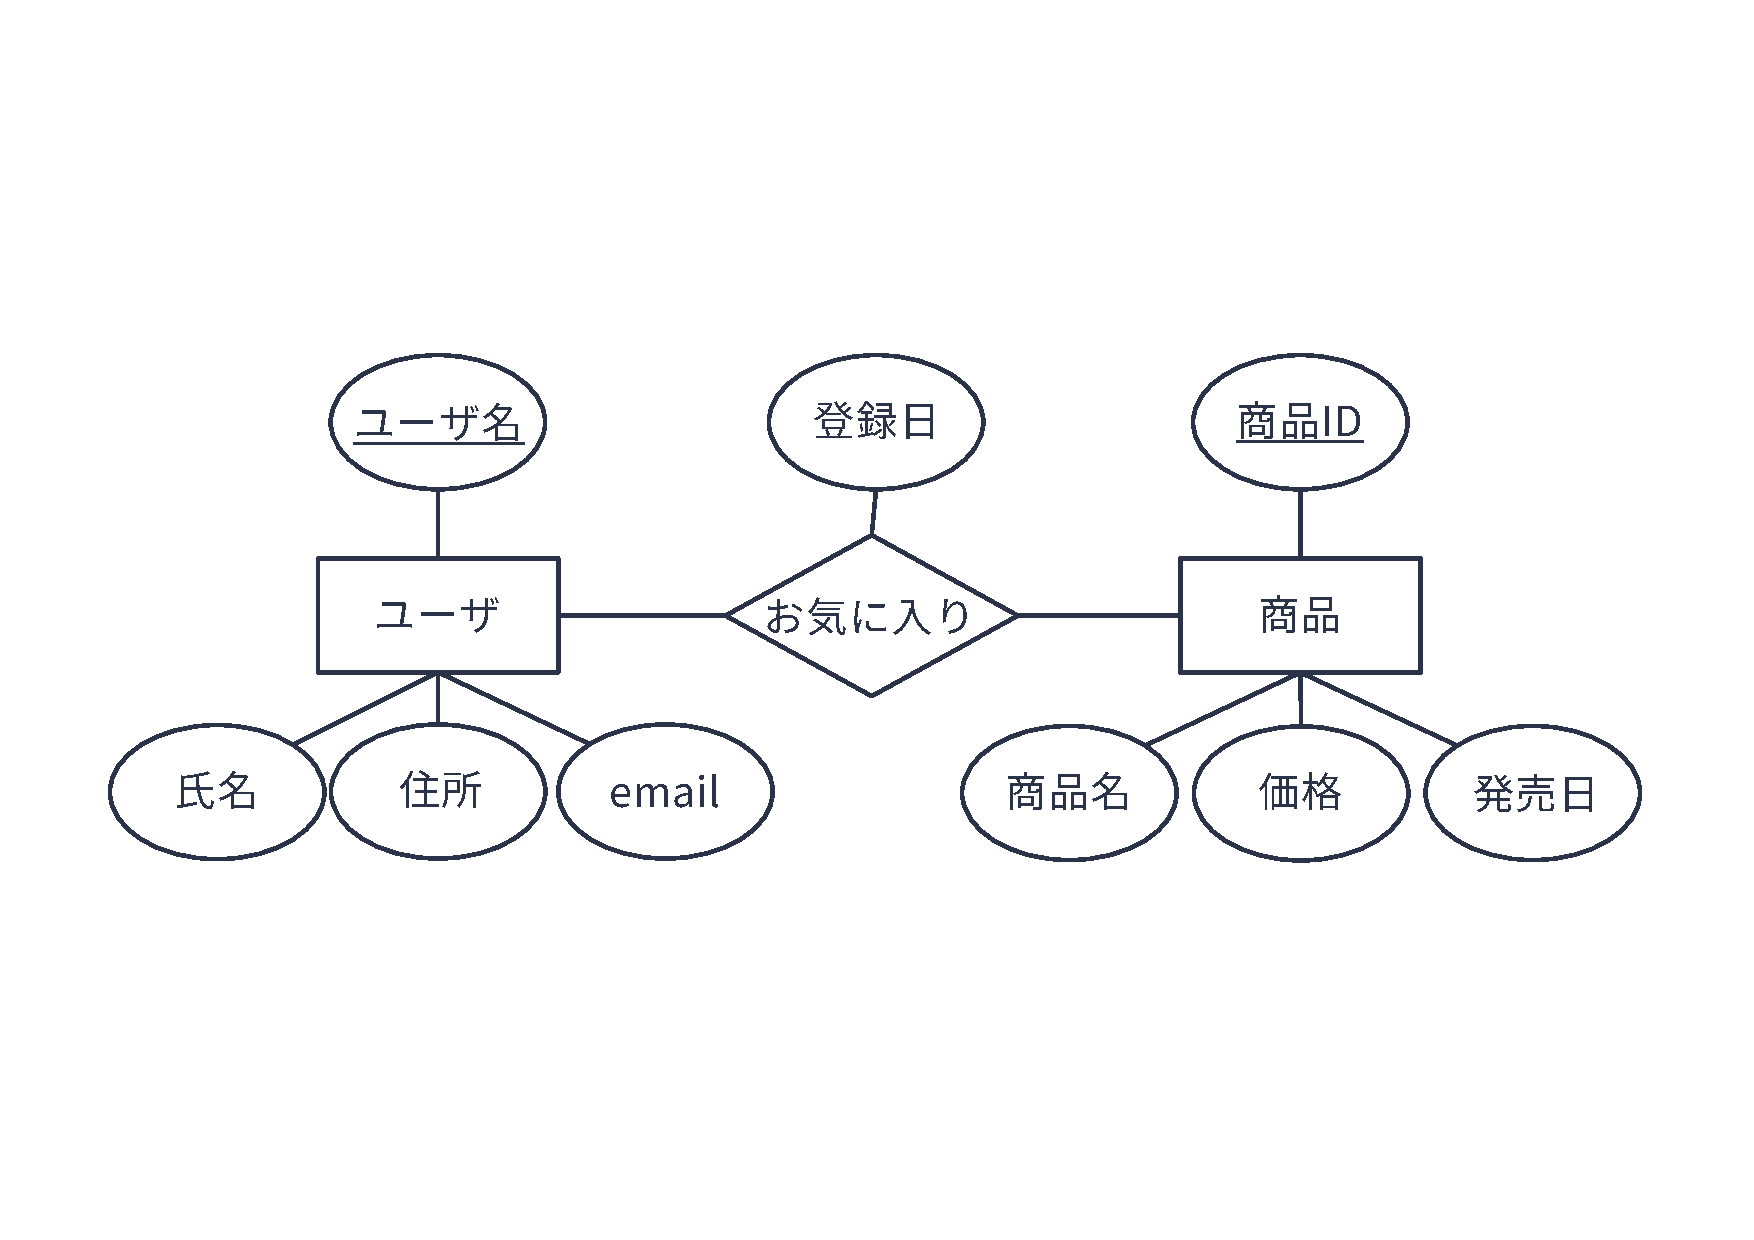
\includegraphics[width=0.9\textwidth]{figure/er-model/erd-relation1.pdf}
  \caption{多対多の関連型「お気に入り」}
  \label{fig:erd-relation1}
\end{figure}
図\ref{fig:erd-relation1}では，実体型「ユーザ」と「商品」は関連型「お気に入り」を介して多対多の関連でつながっています．

このような「多対多」の関連を関係スキーマに変換する場合は，関連を一意に識別するために，\strong{関連型につながるすべての実体型の主キーを集めたもの}を関連型の主キーとします．
図\ref{fig:erd-relation1}の場合，実体型「ユーザ」の主キーは\graybox{ユーザ名}，「商品」の主キーは\graybox{商品ID}であるため，関連型「お気に入り」の主キーは\graybox{\{ユーザ名, 商品ID\}}となります\footnote{このように属性の組みあわせによって構成された主キーは複合主キーと呼ばれます．複合主キーは理論上正しいのですが，実務では管理を容易にするためにシステムが自動的に付与する人工的な主キー「代理キー（surrogate key）」を持たせることがあります．代理キーの例としては，連番や重複しない文字列（UUID）などが挙げられます}．
結果的に，関連型「お気に入り」は以下のような関係スキーマに変換されます．
\begin{equation}
  \text{お気に入り}(\underline{\text{ユーザ名}, \text{商品ID}}, \text{登録日})
\end{equation}

ところで，関連型の関係スキーマの主キーは関連している実体型の主キーから構成されるため，対象となる関連型および実体型を変換した関係スキーマの間には参照整合制約が生じます．
つまり，関連型の主キーは，関連している（つながっている）実体型に対する外部キーとなります．
例えば，先の例の関係「お気に入り」の主キーである\graybox{ユーザ名}と\graybox{商品ID}は，関係「ユーザ」および「商品」に対する外部キーになります．
「お気に入り」の主キーである\graybox{ユーザ名}と\graybox{商品ID}の値は，必ず関係「ユーザ」の\graybox{ユーザ名}の属性値，「商品」の\graybox{商品ID}の属性値として存在している必要があります．
よって，上記関連型を関係スキーマに変換したときには，
\begin{eqnarray}
  \text{ユーザ}(\underline{\text{ユーザ名}}, \text{氏名}, \text{住所}, \text{email}) \label{eq:user}\\
  \text{商品}(\underline{\text{商品ID}}, \text{商品名}, \text{価格}, \text{発売日}) \label{eq:product}\\
  \text{お気に入り}(\underline{\text{ユーザ名}, \text{商品ID}}, \text{登録日}) \label{eq:favorite}\\
  \text{お気に入り.ユーザ名} \subseteq \text{ユーザ.ユーザ名} \label{eq:favorite-fk1}\\
  \text{お気に入り.商品ID} \subseteq \text{商品.商品ID} \label{eq:favorite-fk2}
\end{eqnarray}
が参照整合性制約を含めた関係スキーマとなります．


\subsubsection{多重度が「多対1」の場合}
\figure[tb]
  \centering
  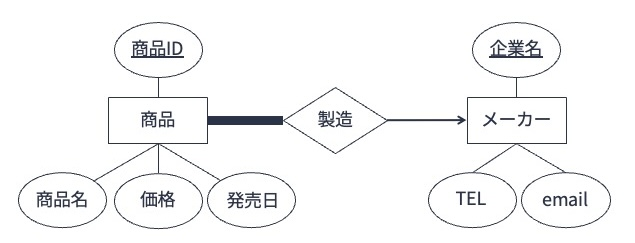
\includegraphics[width=0.9\textwidth]{figure/er-model/erd-relation2.jpg}
  \caption{多対1の関連型「製造」}
  \label{fig:erd-relation2}
\endfigure

図\ref{fig:erd-relation2}では，実体型「商品」と「メーカー」は関連型「製造」を介して多対1の関連でつながっています．
すなわち，実体集合「商品」の実体要素が決まれば，それに対応する実体集合「メーカー」の実体要素が必ず1つ特定されることになります．

このような「多対1」の関連型の場合，矢印のついていない側の実体の主キーの値が決まれば，矢印のついている側の実体が一意に特定されると同時に関連の要素も一意に特定されます．
そのため，関係スキーマに変換する場合は，\strong{関連型につながる，矢印のついていない側の実体型の主キー}を関連型の主キーとします．

図\ref{fig:erd-relation2}を関係スキーマに変換すると，以下のようになります．
関係「製造」において\graybox{企業名}が属性になりますが，主キーにはならない（含まれない）ことに注意しましょう．
\begin{eqnarray}
  \text{商品}(\underline{\text{商品ID}}, \text{商品名}, \text{価格}, \text{発売日}) \\
  \text{メーカー}(\underline{\text{企業名}}, \text{TEL}, \text{email}) \\
  \text{製造}(\underline{\text{商品ID}}, \text{企業名}) \\
  \text{製造.商品ID} \subseteq \text{商品.商品ID}\\
  \text{製造.企業名} \subseteq \text{メーカー.企業名}
\end{eqnarray}

\subsubsection{多重度が「1対1」の場合}
\figure[tb]
  \centering
  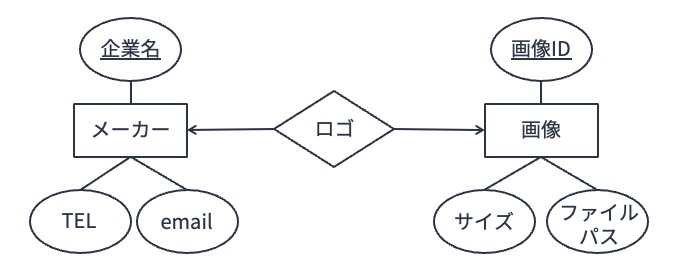
\includegraphics[width=0.9\textwidth]{figure/er-model/erd-relation3.jpg}
  \caption{1対1の関連型「ロゴ」}
  \label{fig:erd-relation3}
\endfigure
図\ref{fig:erd-relation3}では，実体型「メーカー」と「画像」は関連型「ロゴ」を介して1対1の関連でつながっています．

このような「1対1」の関連型の場合，関連している\strong{いずれか}の実体型の主キーの値が決まれば，関連の要素も一意に特定されます．
そのため，関係スキーマに変換する場合は，\strong{関連型につながる，いずれかの実体型の主キー}を関連型の主キーとします．

図\ref{fig:erd-relation3}を関係スキーマに変換すると，以下のようになります．
関係「ロゴ」においては，\graybox{画像ID}が属性になるが主キーにならない（含まれない）ことに注意しましょう．
\begin{eqnarray}
  \text{メーカー}(\underline{\text{企業名}}, \text{TEL}, \text{email}) \\
  \text{画像}(\underline{\text{画像ID}}, \text{ファイル名}, \text{サイズ}) \\
  \text{ロゴ}(\underline{\text{企業名}}, \text{画像ID}) \\
  \text{ロゴ.企業名} \subseteq \text{メーカー.企業名}\\
  \text{ロゴ.画像ID} \subseteq \text{画像.画像ID}
\end{eqnarray}


\subsection{変換パターン3：汎化・継承}
実体型$E_1$を継承した実体型$E_2$を関係スキーマに変換するには，実体型と同じ変換方法を用いればよいです．
すなわち
\begin{itemize}
\item 継承先の実体型名を関係スキーマの関係名
\item 継承元の実体型のキーを関係スキーマのキー
\item 継承先の実体型の属性を関係スキーマの属性
\end{itemize}
に対応させればよいです．
継承先の実体型の主キーは継承元の実体型の主キーとすることに注意しましょう．

\figure[tb]
  \centering
  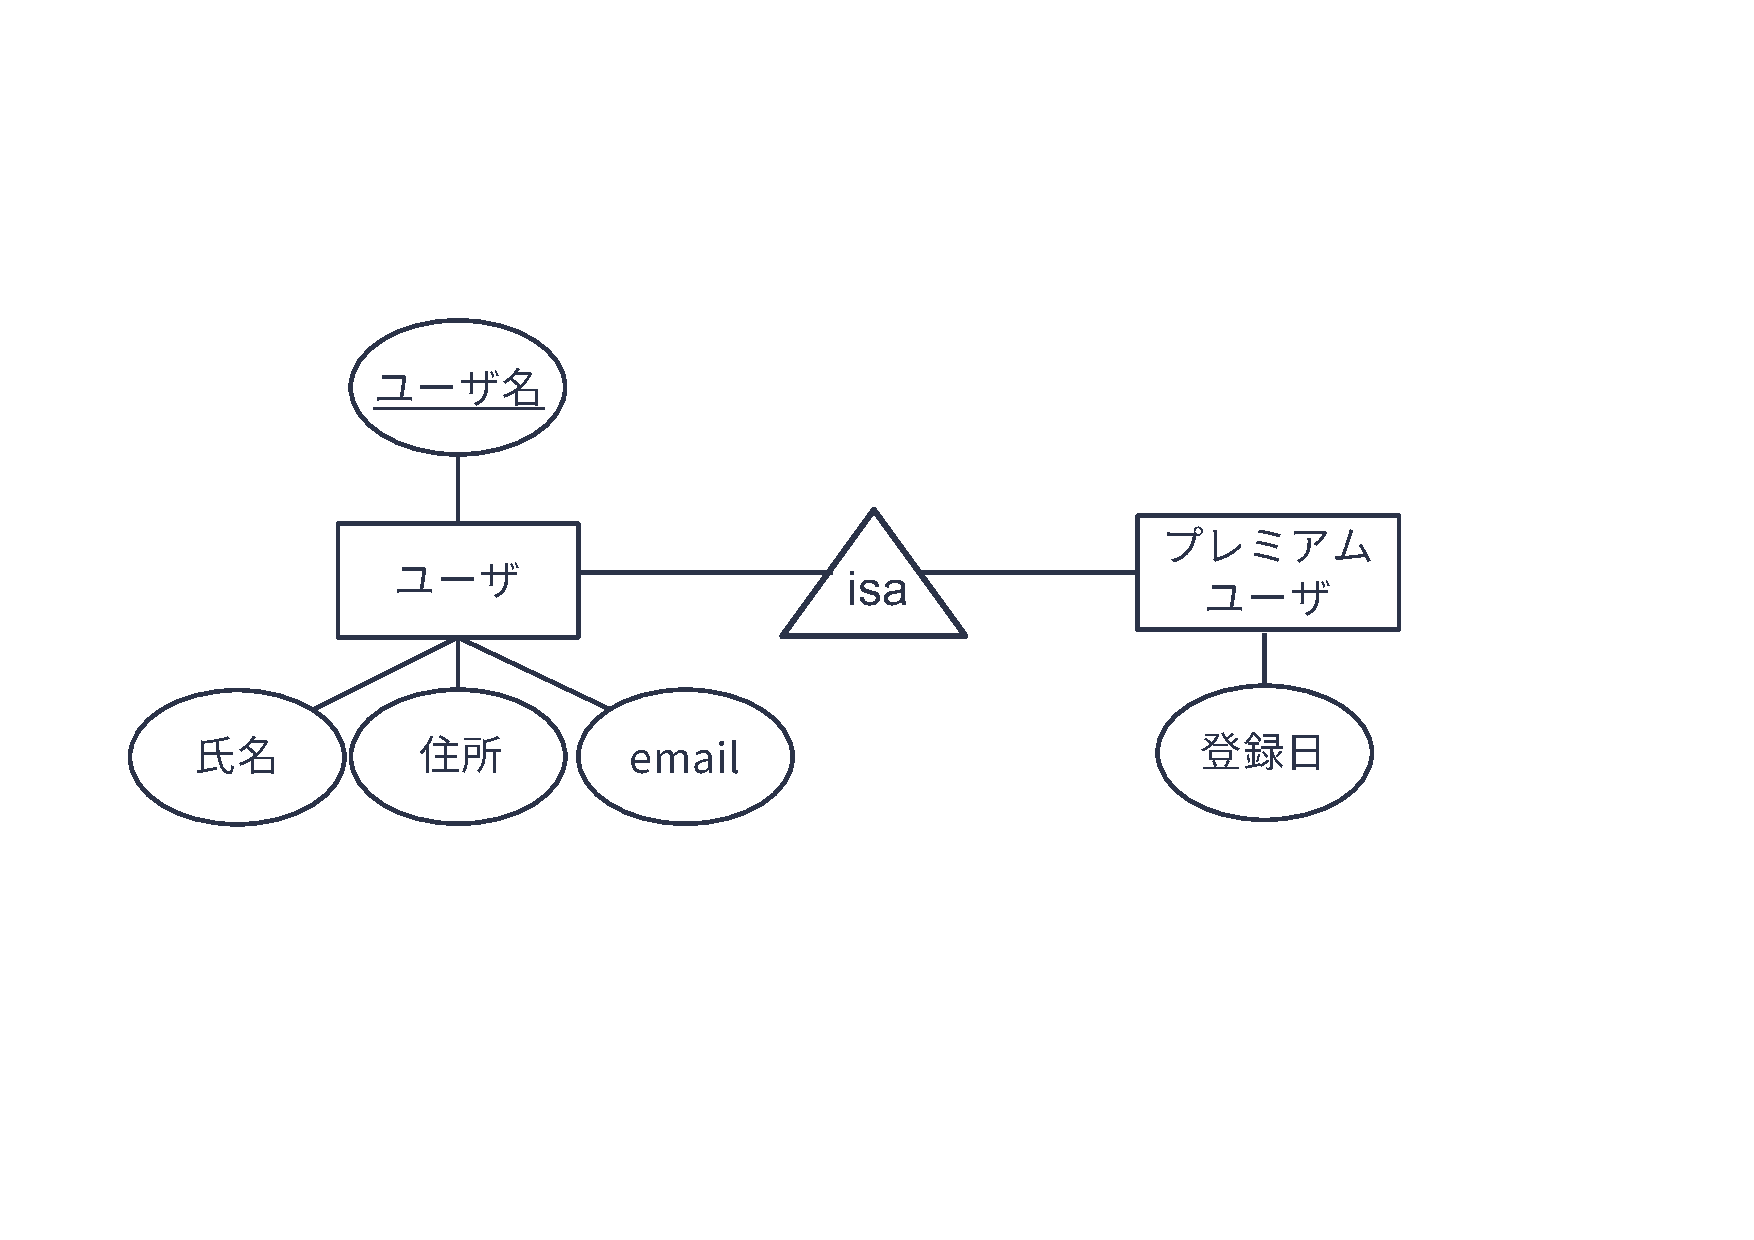
\includegraphics[width=0.8\textwidth]{figure/er-model/erd-inheritance.pdf}
  \caption{実体型「ユーザ」を継承した実体型「プレミアムユーザ」}
  \label{fig:erd-inheritance}
\endfigure
図\ref{fig:erd-inheritance}に示した実体型「プレミアムユーザ」は，以下のような関係スキーマに変換されます．
\begin{equation}
  \text{プレミアムユーザ}(\underline{\text{ユーザ名}}, \text{登録日})
\end{equation}


\subsection{変換パターン4：弱実体型と弱関連型}
\figure[tb]
  \centering
  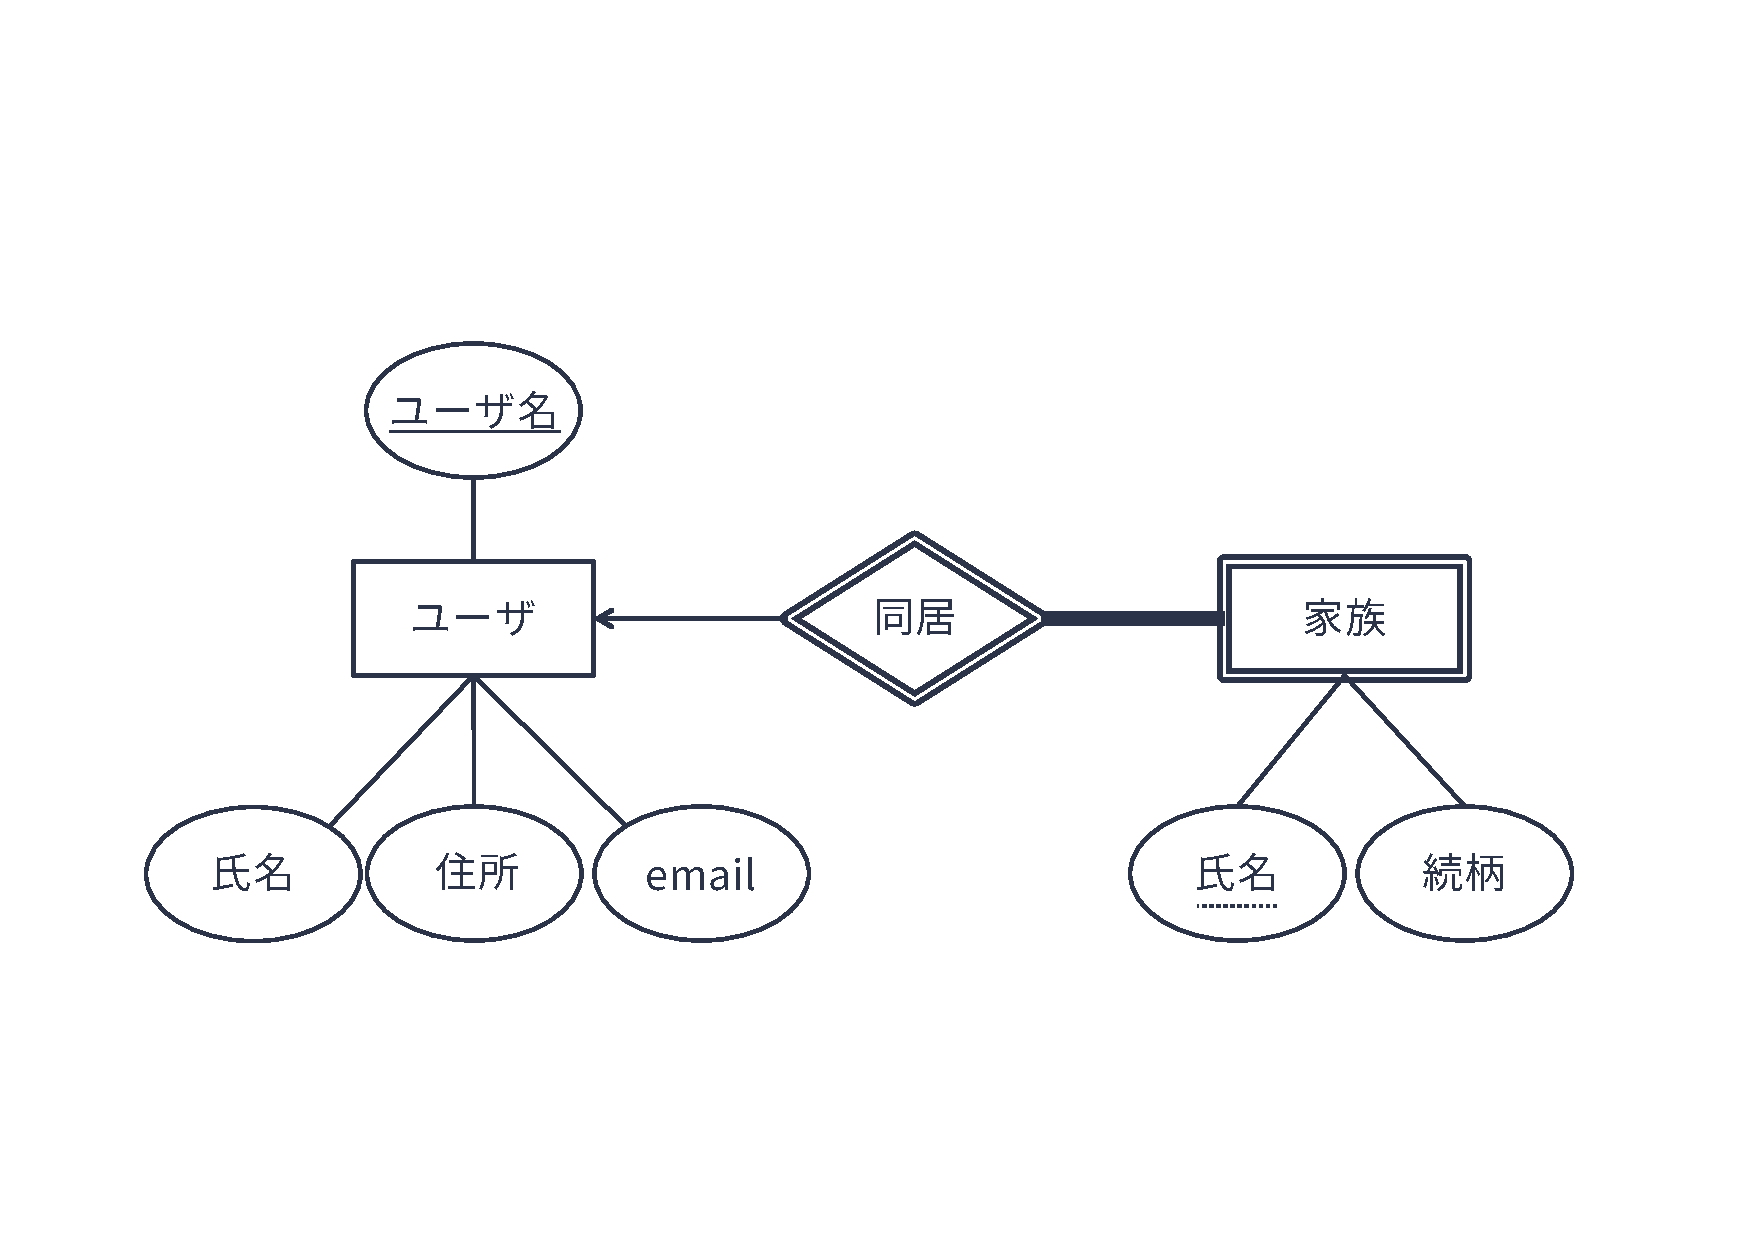
\includegraphics[width=0.9\textwidth]{figure/er-model/weak-entity.pdf}
  \caption{弱実体型「家族」と弱関連型「所属」}
  \label{fig:weak-entity-relation}
\endfigure
図\ref{fig:weak-entity-relation}のような弱実体・弱関連の関係スキーマへの変換はややトリッキーです．
弱実体は自らの属性だけでは一意に特定できないため，弱関連型を通じてつながる（所有）実体型の主キーと自らの属性（部分キー）をセットにして主キーとする必要がありました．
このことを踏まえて，弱実体型は以下のように関係スキーマに変換します．
\begin{itemize}
\item 弱実体型の名前を関係スキーマの関係名にする
\item 弱実体型の部分キーおよび弱実体型とつながる（所有）実体型の主キーをセットにしたものを関係の主キーとする
\item 弱実体型の属性を関係スキーマの属性とする
\end{itemize}

図\ref{fig:weak-entity-relation}の弱実体型「家族」は以下のような関係スキーマに変換されます．
\begin{equation}
  \text{家族}(\underline{\text{ユーザ名}, \text{氏名}}, \text{続柄})
\end{equation}

なお，弱実体型の主キーを構成する要素のうち，部分キーでない方は別の実体型の主キーを借りているため，参照整合性制約が生じます．
先の例の弱実体型「家族」であれば，\graybox{ユーザ名}が外部キーに相当します．
そのため，以下のような参照整合性制約を関係スキーマに加える必要があります．
\begin{equation}
  \text{家族.ユーザ名} \subseteq \text{ユーザ.ユーザ名}
\end{equation}

弱関連型は
\begin{itemize}
\item 弱関連型名を関係スキーマの関係名
\item 自らの部分キーと弱関連型でつながる（所有）実体型の主キーのセットを関係スキーマの主キー
\item 弱関連型の属性を関係スキーマの属性
\end{itemize}
に対応させることで関係スキーマに変換します．

図\ref{fig:weak-entity-relation}の弱関連型「同居」は，以下のような関係スキーマに変換されます．
\begin{eqnarray}
  \text{同居}(\underline{\text{ユーザ名}, \text{氏名}}) \\
  \text{同居.ユーザ名} \subseteq \text{ユーザ.ユーザ名} \\
  \text{同居.氏名} \subseteq \text{家族.氏名} \\
\end{eqnarray}

ところで，弱実体型「家族」は，弱関連型「同居」に対する参加制約が全体的です．
また，弱実体型「家族」に対応する関係スキーマ「家族」の属性は弱関連型「同居」に対応する関係スキーマ「同居」の属性を包含しています．
これは，関係「家族」があれば関係「同居」は把握でき，関係「同居」は不要であることを意味します．
結果的に，関係「同居」は削除できます．


\section{レコードを追加，修正，削除するためのSQL}
関係スキーマが定義できれば，いよいよ関係データベースにレコードの追加，修正，削除が可能となります．
レコードの追加，修正，削除には，\ref{chap:sql-part1}で紹介した関係データベースの問い合わせ言語であるSQLを用います．
以下では，SQLを用いてレコードの追加，修正，削除を行うための基本的な方法を説明します．

\subsection{テーブルの定義}
レコードを追加するには，まず関係データベース内にレコードを追加するテーブルを定義する必要があります．
これまでに説明してきた関係スキーマは，このテーブル定義に活かされます．

SQLでテーブルの定義を行うには，\graybox{CREATE TABLE}文を用います．
\graybox{CREATE TABLE}文の構文はコード\ref{code:create-table-structure}のようになっています．
ここで，テーブル名は関係スキーマにおける関係名，列名は属性名に対応します．
主キーや外部キーは，それぞれ関係スキーマで指定している主キー制約，参照整合性制約に対応します．
\begin{figure}[h]
    \begin{minted}[gobble=1,
        bgcolor=background,
        fontsize=\small,
        linenos=false,
        xleftmargin=0em]{sql}

    CREATE TABLE テーブル名 (
        列名1 データ型 [制約],
        列名2 データ型 [制約],
        ...
        [主キー]
        [外部キー]
    );
    \end{minted}
    \captionsetup{name=コード}
    \caption{CREATE TABLE文の構文．[ ]は省略可能な要素を示す．}
    \label{code:create-table-structure}
\end{figure}

データ型は\ref{chap:relational-data-model}で説明したドメイン制約に対応するものです．
SQLでは整数や文字列など，単純なドメイン制約を指定するデータ型が用意されています．
代表的なデータ型は以下の通りです：
\begin{itemize}
\item \graybox{INT}：整数型
\item \graybox{VARCHAR(n)}：（最大$n$文字の長さの）文字列型
\item \graybox{FLOAT}：浮動小数点数型
\item \graybox{BOOLEAN}：真偽値型
\item \graybox{DATETIME}：時刻を併せ持つ日付型
\end{itemize}
ドメイン制約では属性値は「整数でなければならない」といった単純な制約だけでなく，
\begin{itemize}
\item 0以上10000以下の整数でなければならない
\item xxx，yyy，zzzのいずれかでなければならない
\item @xxxx.comの形式の文字列で終わらなければならない
\end{itemize}
といった複雑な制約が必要になることもあります．
このような複雑な制約を\graybox{CREATE TABLE}文で指定するには，\graybox{CREATE DOMAIN}文でドメインを定義し，そのドメインをテーブル定義のデータ型に指定する方法があります．
これについては本書のレベルを超える内容になるため，ここでの説明は割愛します．

\graybox{CREATE TABLE}文における列名の「制約」には，その列に対する様々な制約を指定することができます．
代表的な制約は以下の通りです：
\begin{itemize}
\item \graybox{NOT NULL}：NULL値を許さない制約
\item \graybox{UNIQUE}：重複する値を許さない制約
\item \graybox{PRIMARY KEY}：主キー制約
\item \graybox{REFERENCES}：参照整合性制約（外部キーの指定）
\end{itemize}

例えば，式\ref{eq:user}で定義した関係スキーマ「ユーザ」，式\ref{eq:product}で定義した関係スキーマ「商品」を用いてテーブル定義するには，コード\ref{code:create-table}のような\graybox{CREATE TABLE}文を用います．
\begin{figure}[h]
    \begin{minted}[gobble=1,
        bgcolor=background,
        fontsize=\small,
        linenos=false,
        xleftmargin=0em]{sql}

    CREATE TABLE ユーザ (
        ユーザ名 VARCHAR(100) PRIMARY KEY, --- コメント: 文字列長は最大100文字とする
        氏名 VARCHAR(100) NOT NULL,
        住所 VARCHAR(100) NOT NULL,
        email VARCHAR(100) NOT NULL
    );

    CREATE TABLE 商品 (
        商品ID VARCHAR(100) PRIMARY KEY,
        商品名 VARCHAR(100) NOT NULL,
        価格 INT NOT NULL,
        発売日 DATETIME NOT NULL
    );

    \end{minted}
    \captionsetup{name=コード}
    \caption{テーブル「ユーザ」「商品」を定義するCREATE TABLE文の例．}
    \label{code:create-table}
\end{figure}

主キーおよび外部キーの指定は，列定義の中で指定する方法と，テーブル全体の制約として指定する方法があります．
主キーが複数の列の組みあわせで構成されるなど，複雑な主キーや外部キーを指定する場合は，テーブル全体の制約として指定する方法が適しています．
コード\ref{code:create-table2}は，式\ref{eq:favorite}-\ref{eq:favorite-fk2}で定義した関係スキーマ「お気に入り」をテーブル定義するための\graybox{CREATE TABLE}文の例です．
\begin{figure}[h]
    \begin{minted}[gobble=1,
        bgcolor=background,
        fontsize=\small,
        linenos=false,
        xleftmargin=0em]{sql}

    CREATE TABLE お気に入り (
        ユーザ名 VARCHAR(100) NOT NULL,
        商品ID VARCHAR(100) NOT NULL,
        登録日 DATETIME NOT NULL,
        --- コメント: 主キーはユーザ名と商品IDの組みあわせ
        PRIMARY KEY (ユーザ名, 商品ID),
        --- テーブル「お気に入り」の「ユーザ名」はテーブル「ユーザ」の「ユーザ名」に対する外部キーとなる
        FOREIGN KEY (ユーザ名) REFERENCES ユーザ(ユーザ名)
    );

    \end{minted}
    \captionsetup{name=コード}
    \caption{テーブル「お気に入り」を定義するSQL文の例．}
    \label{code:create-table2}
\end{figure}


\subsection{レコードの追加}
テーブルにレコードを追加するには，\graybox{INSERT}文を用います．
\graybox{INSERT}文の構文はコード\ref{code:insert-into-structure}のようになっています．
\begin{figure}[h]
    \begin{minted}[gobble=1,
        bgcolor=background,
        fontsize=\small,
        linenos=false,
        xleftmargin=0em]{sql}

    INSERT INTO
        テーブル名 (列名1, 列名2, ...)
    VALUES
        (レコード1件目の属性1の値, 属性2の値, ...),
        (レコード1件目の属性2の値, 属性2の値, ...)
        ... ;
    \end{minted}
    \captionsetup{name=コード}
    \caption{INSERT文の構文}
    \label{code:insert-into-structure}
\end{figure}

コード\ref{code:insert-into-example}は，先ほど取り上げた\graybox{商品}テーブルに3件のレコードを追加するためのSQL文の例です．
\begin{figure}[h]
    \begin{minted}[gobble=1,
        bgcolor=background,
        fontsize=\small,
        linenos=false,
        xleftmargin=0em]{sql}

    INSERT INTO
        商品 (商品ID, 商品名, 価格, 発売日)
    VALUES
        ('P001', 'はーいお茶', 130, '1989-02-01 09:00:00'),
        ('P002', 'きのこの里', 230, '2019-08-06 10:00:00'),
        ('P003', 'のど飴', 170, '2016-02-16 14:30:00');

    \end{minted}
    \captionsetup{name=コード}
    \caption{テーブル「商品」にレコードを追加するSQL文の例}
    \label{code:insert-into-example}
\end{figure}

\subsection{レコードの削除}
テーブル中のレコードを削除するには，\graybox{DELETE}文を用います．
\graybox{DELETE}文の構文はコード\ref{code:delete-structure}のようになっています．
\begin{figure}[h]
    \begin{minted}[gobble=1,
        bgcolor=background,
        fontsize=\small,
        linenos=false,
        xleftmargin=0em]{sql}

    DELETE FROM
        テーブル名
    WHERE
        条件 ;

    \end{minted}
    \captionsetup{name=コード}
    \caption{DELETE文の構文}
    \label{code:delete-structure}
\end{figure}

コード\ref{code:delete-example}は，先ほど取り上げた\graybox{商品}テーブルから特定のレコードを削除するためのSQL文の例です．
\begin{figure}[h]
    \begin{minted}[gobble=1,
        bgcolor=background,
        fontsize=\small,
        linenos=false,
        xleftmargin=0em]{sql}

    DELETE FROM
        商品
    WHERE
        価格 <= 100;

    \end{minted}
    \captionsetup{name=コード}
    \caption{テーブル「商品」から価格が100円以下のレコードを削除するSQL文の例}
    \label{code:delete-example}
\end{figure}


\subsection{レコードの修正}
テーブル中のレコードを修正するには，\graybox{UPDATE}文を用います．
\graybox{UPDATE}文の構文はコード\ref{code:update-structure}のようになっています．
\begin{figure}[h]
    \begin{minted}[gobble=1,
        bgcolor=background,
        fontsize=\small,
        linenos=false,
        xleftmargin=0em]{sql}

    UPDATE
        テーブル名
    SET
        列名1 = 値1,
        列名2 = 値2,
        ...
    WHERE
        条件 ;
    \end{minted}
    \captionsetup{name=コード}
    \caption{UPDATE文の構文}
    \label{code:update-structure}
\end{figure}

コード\ref{code:update-example}は，先ほど取り上げた\graybox{商品}テーブルの中で「商品ID」が\graybox{P002}のレコードを価格を1割引きしたものに修正するSQL文の例です．
\begin{figure}[h]
    \begin{minted}[gobble=1,
        bgcolor=background,
        fontsize=\small,
        linenos=false,
        xleftmargin=0em]{sql}

    UPDATE
        商品
    SET
        価格 = 価格 * 0.9
    WHERE
        商品ID = 'P002';

    \end{minted}
    \captionsetup{name=コード}
    \caption{テーブル「商品」中の「商品ID」がP002のレコードの価格を1割引きした値に修正するSQL文の例}
    \label{code:update-example}
\end{figure}

% ---------------------------------------
\section{クイズ}
% ---------------------------------------

Apple Music\footnote{https://music.apple.com/}やSpotify\footnote{https://open.spotify.com/}，LINE MUSIC\footnote{https://music.line.me/}などのサブスクリプション型音楽ストリーミングサービスでは，月額や年額でサービス使用料を支払うことで，好きなアーティストの好きな楽曲を好きなだけ聴くことができます．
ユーザは「プレイリスト」と呼ばれる，あるテーマをもとに楽曲を集めたリストを作成・公開することができます．
また，ユーザは別のユーザをフォローし，そのユーザが新しいプレイリストを作成すると通知を受け取ることもできます．

下記クイズでは，架空のサブスクリプション型音楽ストリーミングサービス「Orange Music」の実体関連モデルについて考えてみましょう．
なおQ2以降のクイズの回答は，直前のクイズの回答を前提としています．

\subsubsection{Q1. 実体（1/3）}
Orange Musicの「ユーザ」は「ユーザID」「氏名」「性別」「誕生日」「電話番号」を持ちます．
この状況を実体関連図で表現しなさい．

\subsubsection{Q2. 実体（2/3）}
Orange Musicの「楽曲」は「楽曲ID」「楽曲名」「ジャンル」「長さ」を持ちます．
この状況を実体関連図で表現しなさい．

\subsubsection{Q3. 実体（3/3）}
Q2で定義した実体型「楽曲」の実体の例を2，3挙げなさい．
なお，属性の値は適当に決めてよいです．

\subsubsection{Q4. 関連（1/3）}
Orange Musicの「アーティスト」は「アーティストID」「アーティスト名」を持ちます．
「アーティスト」は作成した「楽曲」をOrange Musicに「公開」します．
「公開」には「公開日」が記録されます．
この状況を実体関連図で表現しなさい．

\subsubsection{Q5. 関連（2/3）}
Orange Musicの「ユーザ」は「プレイリスト」に「作成」することがあります．
「プレイリスト」は「プレイリストID」「プレイリスト名」を持ちます．
プレイリスト「作成」時には「作成日」が記録されます．
作成された「プレイリスト」には「楽曲」を「追加」することができます．
「追加」には楽曲がプレイリストに「追加された日」が記録されます．
この状況を実体関連図で表現しなさい．

\subsubsection{Q6. 関連（3/3）}
Orange Musicの「ユーザ」は別の「ユーザ」を「フォロー」します．
「フォロー」は「フォロー日」が記録されます．
この状況を実体関連図で表現しなさい．

\subsubsection{Q7. 参加制約}
Q6までに作成した実体関連図において，参加が「全体的」となる実体型と関連型のペアを考え，それを実体関連図に反映させなさい．

\subsubsection{Q8. 多重度（1/4）}
Q7で作成した実体関連図に，以下の設定を追加反映しなさい．

\begin{framed}
「レーベル」は「レーベル名」「住所」をもつ．
「アーティスト」はいずれか1つの「レーベル」に「所属」し，「レーベル」には何組かの「アーティスト」が「所属」する．
\end{framed}

\subsubsection{Q9. 多重度（2/4）}
Q8で作成した実体関連図に，以下の設定を追加反映しなさい．

\begin{framed}
「アーティスト」はいくつかの「楽曲」を「公開」する．
「楽曲」公開時には必ず「アーティスト」が1名登録される．
「ユーザ」はいくつかの「楽曲」を「プレイリスト」に「追加」する．
ある「プレイリスト」を作成した「ユーザ」は必ず一人である．
\end{framed}

\subsubsection{Q10. 多重度（3/4）}
Q9で作成した実体関連図に，以下の設定を追加反映しなさい．

\begin{framed}
「ユーザ」は気に入った「楽曲」に「いいね」をすることができる．
「ユーザ」は何曲でも「いいね」できる．
「いいね」は「いいねされた日（liked\_at）」が記録される．
\end{framed}

\subsubsection{Q11. 多重度（4/4）}
Q10で作成した実体関連図において「弱実体」「弱関連」になり得るものを特定し，それを実体関連図に反映しなさい．
なお，弱実体の部分キーには点線を付与すること．

\subsubsection{Q12. 汎化・継承}
Q11で作成した実体関連図に，以下の設定を追加反映しなさい．

\begin{framed}
Orange Musicは追加サービスとして「プレミアムユーザ」サービスを開始した．
Orange Musicの「ユーザ」は追加料金を支払うことで「プレミアムユーザ」になることができる．
「プレミアムユーザ」は最大100曲まで「楽曲」を「ダウンロード」できる．
「ダウンロード」には「ダウンロード日」を記録する．
\end{framed}

\subsubsection{Q13. n項関連（1/2）}
Q12で作成した実体関連図に，以下の設定を追加反映しなさい．

\begin{framed}
Orange Musicでは追加サービスとして，アーティストがコンサート等のイベントで演奏した曲目（いわゆるセットリスト）を閲覧できるサービスを開始することにした．
このサービスでは，「アーティスト」がどの「楽曲」をどの「イベント」で「演奏」したのかを閲覧できる．
「イベント」は「イベント名」「場所」「日時」を情報としてもつ．
また，「演奏」にはイベント中の演奏順序を示す「演奏番号」が記録される．
なお，「アーティスト」が「演奏」した「楽曲」は他者が制作した楽曲も含まれる．
\end{framed}


\subsubsection{Q14. n項関連（2/2）}
図\ref{fig:cardinality_constraint}の実体関連図に，以下の設定を追加反映しなさい．
\begin{framed}
 このオンラインショッピングサイトでは，「ユーザ」がどの「商品」を「購入」したかを記録している．
 購入記録においては，購入した「商品」の「数量」や「購入日」の情報を記録している．
\end{framed}

\subsubsection{Q15. 実体関連モデルから関係スキーマへの変換}
図\ref{fig:erd-to-schema}は，架空のショッピングサイトにおける購買履歴を管理するシステムの実体関連図です．
この実体関連図を関係スキーマに変換しなさい．
\figure[htb]
    \centering
    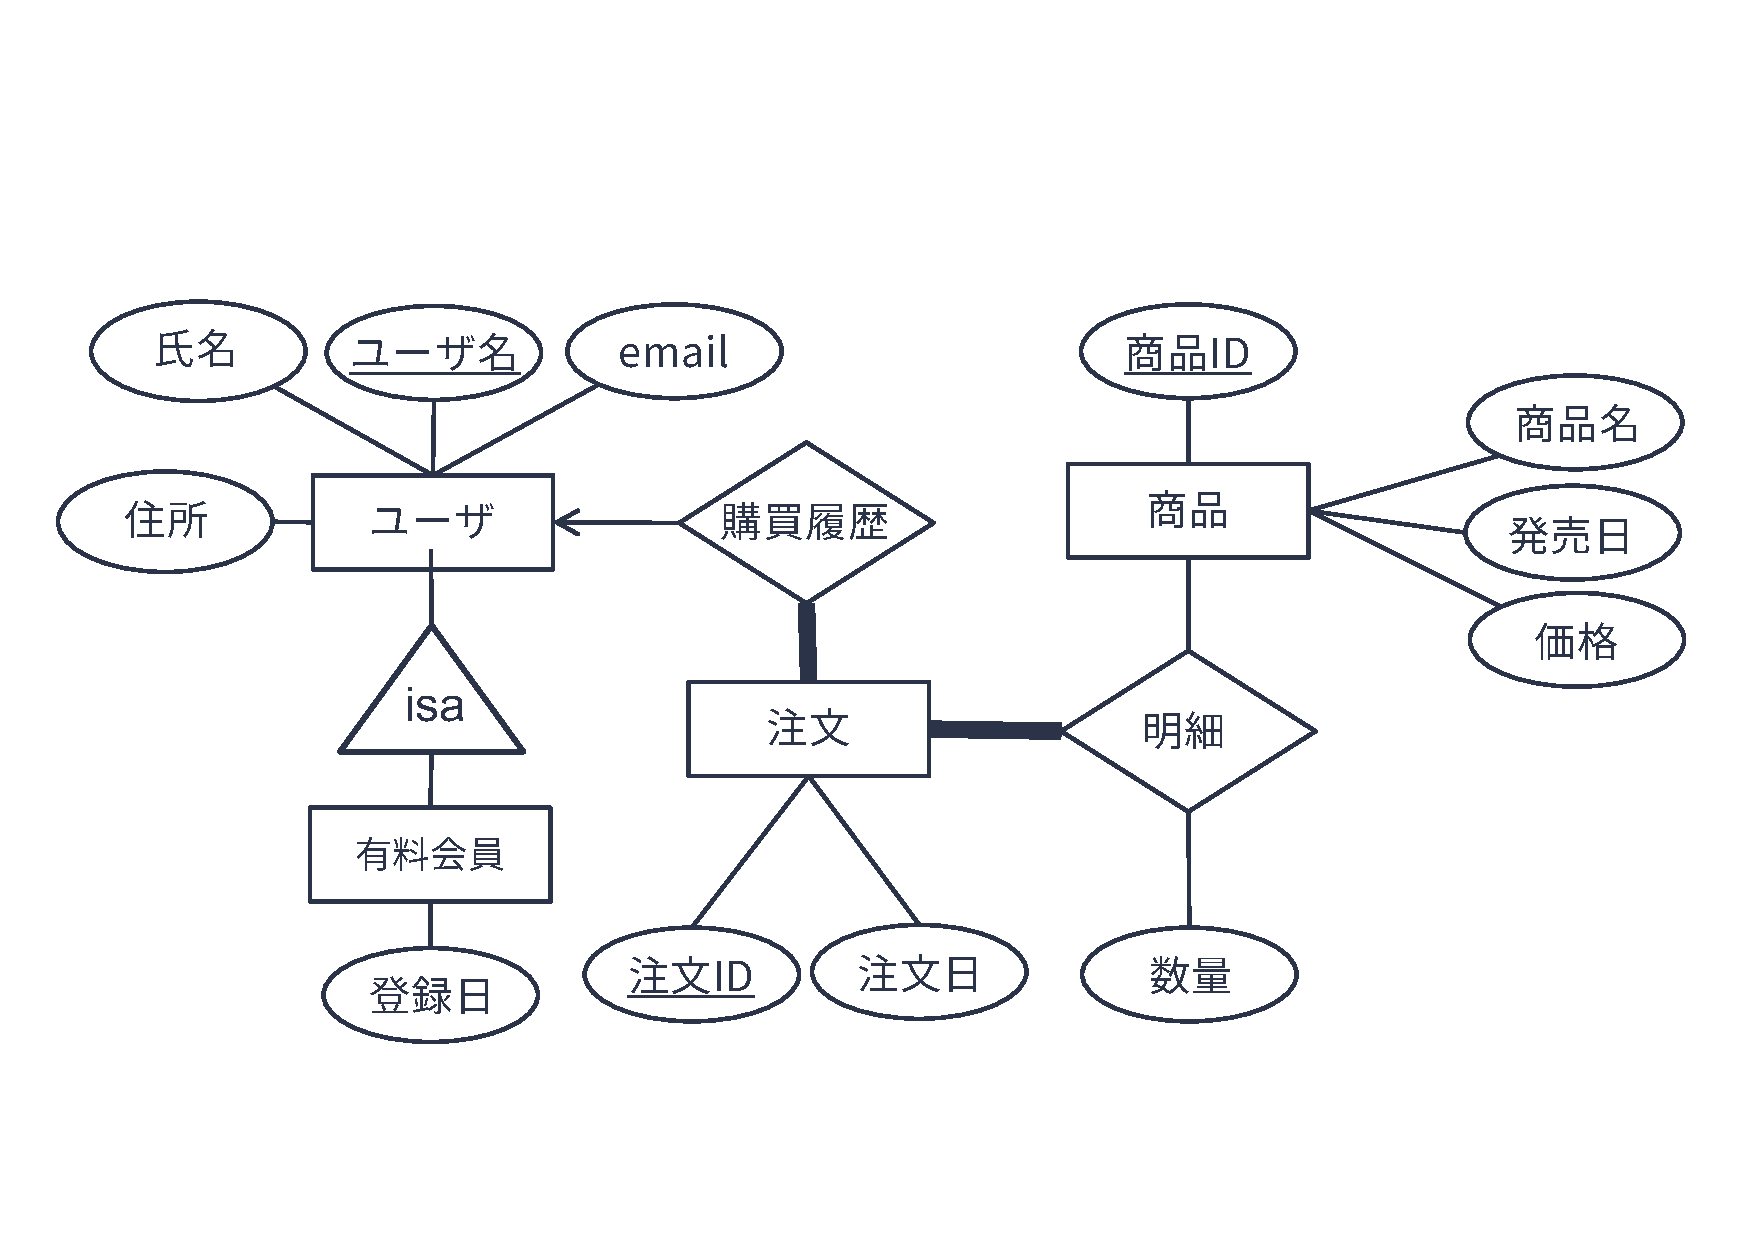
\includegraphics[width=1.0\textwidth]{figure/er-model/erd-to-schema.pdf}
    \caption{購買履歴を管理するシステムの実体関連図}
    \label{fig:erd-to-schema}
\endfigure

% \chapter{関係データベースの設計 -- 正規化}

「IT Text データベースの基礎」（吉川正俊著）\cite{吉川本}で述べられているように，理想的なデータベースは以下の性質を有するデータベーススキーマを持ちます：
\begin{enumerate}
  \item データの冗長性がない
  \item データの一貫性制約の保持が容易である
\end{enumerate}
関係データベースにおいては，上記(1)(2)の要件を満たすように関係スキーマを定義することを\strong{正規化（normalization）}と呼びます．
望ましい関係スキーマ，つまり正規化された関係スキーマが設計できれば，関係データベースから\strong{冗長性が排除され（データの重複がなく），データを正しく矛盾なく管理・処理}できるようになります．

前章では実体関連モデルを用いた関係スキーマの設計方法について説明しましたが，実はこの方法では十分な正規化が保証されません．
実体関連モデルの変換のみで適切な関係スキーマを得るためには，実体関連図の設計段階で正規化を意識した設計を行う必要があり，設計の質は設計者の経験やスキルに依存します．

このような問題を解決するのが，正規化の理論に基づいた関係スキーマの設計方法です．
本章では，実体関連モデルの変換による関係スキーマを補完する，データ従属性に基づく正規化手法について説明します．

% \chapter{索引づけ}
\ref{chap:er-model}章や\ref{chap:normalization}章で説明した実体関連モデルと正規化理論によって，データを正しく矛盾なく管理するための関係データベースを設計することができるようになりました．
しかし，データの正しさをガチガチに担保できるようになっても，問い合わせにかかる待ち時間が長いようではデータベースとして使い物になりません．
利便性が高いデータベースには，データの管理のしやすさに加え，データの処理速度も求められます．

ところで，これまでの章で見てきたように，関係データベースに格納されたデータは，複数のテーブルに分割されていることがほとんどです．
そのため，必要なデータを取得するには，
\begin{itemize}
\item 関係する複数のテーブルを結合し
\item 結合したテーブルのレコードから条件に合致するものを抽出する
\end{itemize}
といった処理が必要となります．
さて，テーブルの結合は，結合元のテーブルの各レコードに対し，結合先のテーブルから条件に合致するレコードを検索してつなぎ合わせる処理であることを思い出してください．
ということは，結合元と結合先のテーブルのレコード数が多いほど，処理が重くなりそうです．
例えば，結合元と結合先のテーブルのレコード数がそれぞれ100万件ある場合，レコードのすべての組み合わせについて条件を満たすかを逐一チェックすると，合計1兆ペアも確認しなければなりません．
確認回数が多いと，それに比例してテーブルの結合にかかる時間は長くなってしまいます．

この問題を解決する技術が\strong{索引づけ（indexing）}です\footnote{データベースの応答速度（クエリ実行時間）を改善する方法としては，索引づけ以外にもクエリ最適化（query optimization）などがあります}．
索引づけを行うことで，データベースは条件に合致するレコードの検索速度を大幅に改善することができます．
本章では，索引づけの基本的な考え方と，索引づけに使われる代表的なデータ構造であるB+木とハッシュ索引について説明します．


\section{関係データの物理的な格納方法}
計算機ではあらゆるデータはゼロイチの2進数で表現され，主記憶装置（メモリ）やハードディスクやSSDのような補助記憶装置のどこかに物理的に格納されています．
このことは，計算機を使う関係データベースにおいても同じです．
関係データベースではすべてのデータはテーブルとして表現されますが，データを補助記憶装置に格納する際，テーブルを構成する複数のレコードはひとまとまりの単位（ブロック）に分割され，記憶装置のどこかに格納されます．

% \begin{notebox}
% 表データをタプル（レコード）単位で分割し格納するデータベースは\strong{行指向データベース（row-oriented database）}と呼ばれます．
% それに対して，属性（列）単位で分割・格納するデータベースは\strong{列指向データベース（column-oriented database）}と呼ばれます．

% 関係データベースのようにレコードの追加や削除を頻繁に行うことが想定されるデータベースにおいては，行指向でデータを格納するほうが効率的です．
% 一方，データの更新が頻繁でなく，属性（列）単位の集約演算を頻繁に行うような場合は，列指向データベースの方が効率的です．
% \end{notebox}

図\ref{fig:data-store}は，「商品」テーブルを（物理的な）記憶媒体に格納する際のイメージ図です．
図のように，「商品」の各レコードは記憶装置の特定の場所にばらばらに格納されます．
SQL文による問い合わせが行われると，関係データベースシステムは条件に合致するレコードが記憶装置のどの場所に保存されているか（アドレス）を調べ，該当する場所から具体的なデータを取得します．

\begin{figure}[tb]
    \centering
    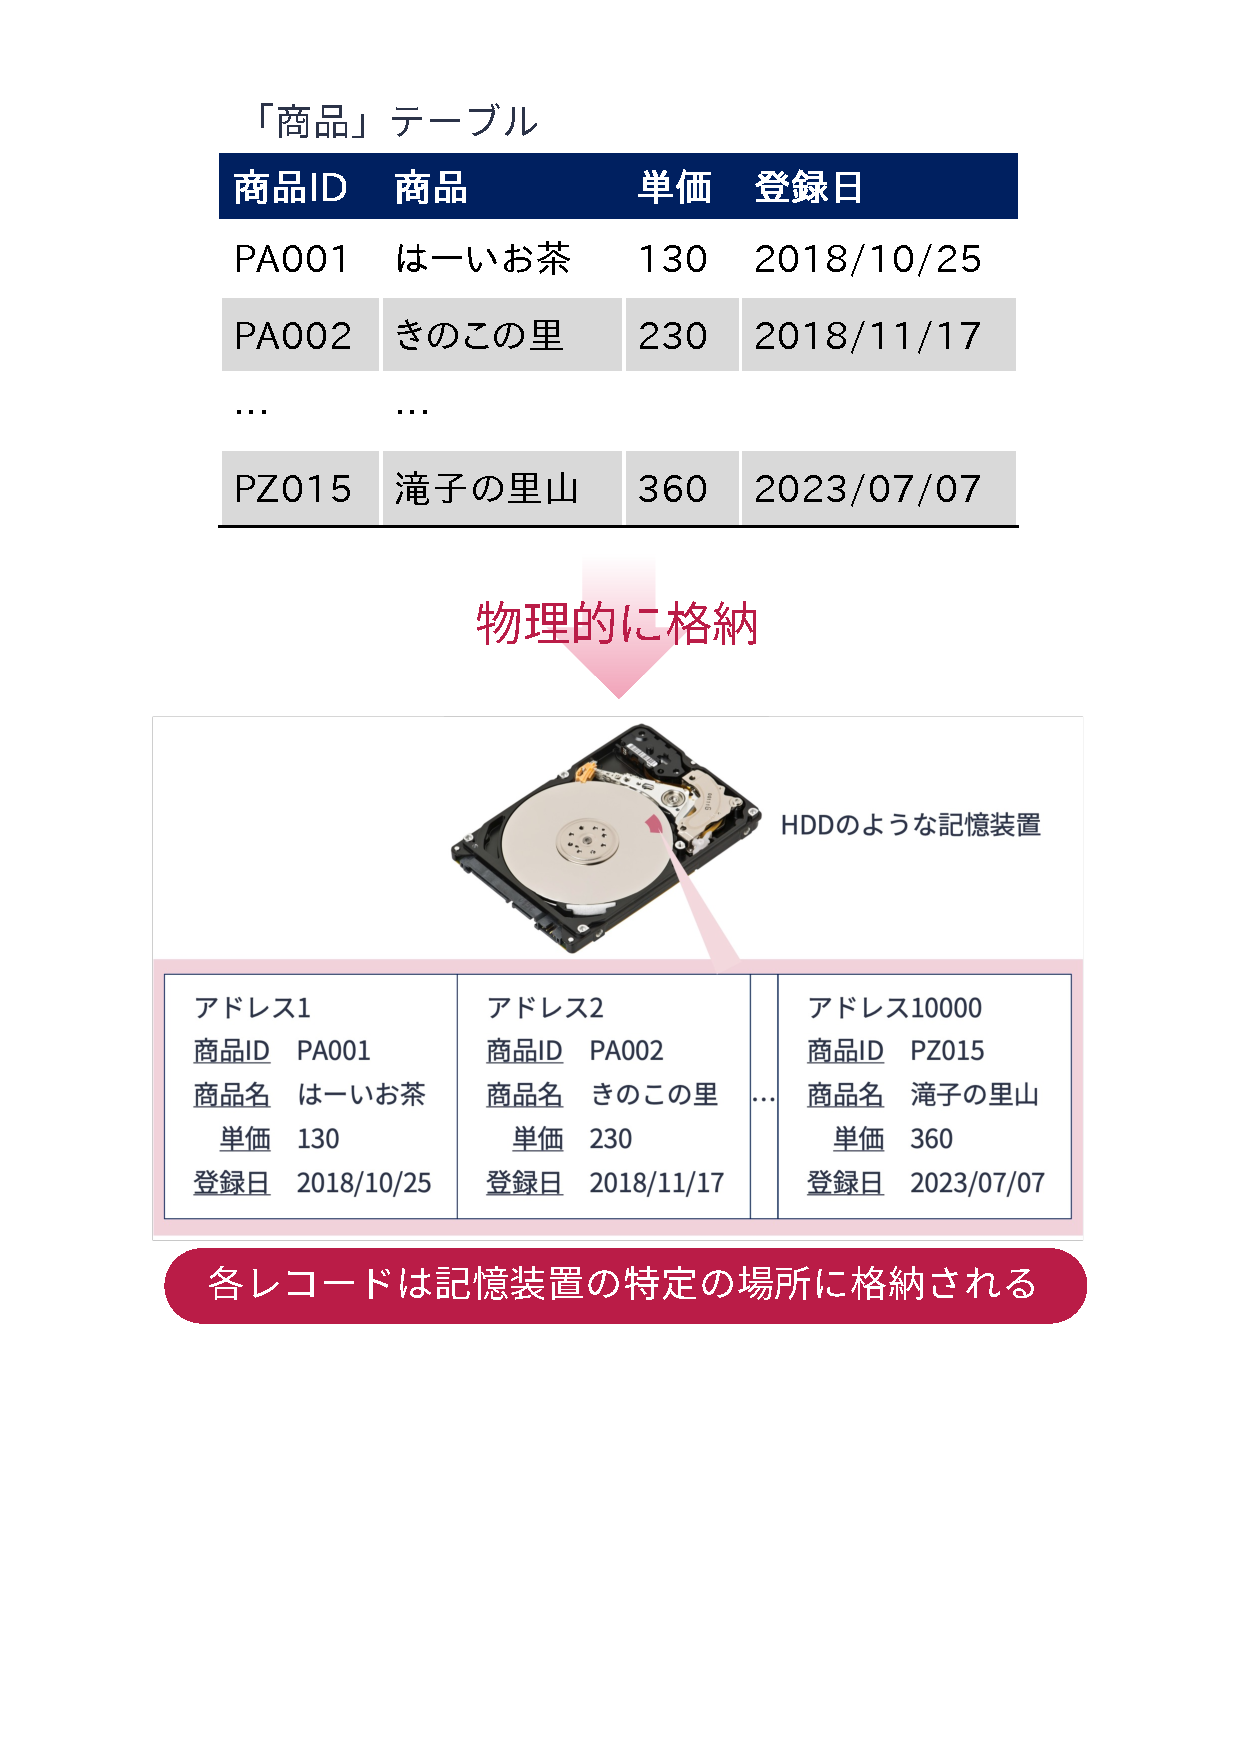
\includegraphics[width=0.8\textwidth]{figure/indexing/data-store.pdf}
    \caption{関係データの物理的な格納方法のイメージ}
    \label{fig:data-store}
\end{figure}


\section{索引}
データベースから条件に合致するレコードを探す方法として，該当するテーブルのレコードが格納されている場所を先頭から1つ1つ調べ上げる方法が考えられます．
この方法では，レコードの数が$N$件ある場合，$N$回確認作業が必要となります．
問い合わせへの応答時間は，確認回数に比例して長くなります．
レコードの数が少ない，つまり$N$が小さい場合は問題となりません．
しかし，ビジネスの現場等で用いられる関係データベースは，膨大な数のレコードを扱います．
計算が得意な計算機とはいえ，数百万，数千万のレコード数を逐次的にチェックするにはそれなりに時間がかかります．

\strong{索引づけ（indexing）}は，レコードの探索時間を改善したいときに有効な方法の1つです．
一般に索引といえば，書籍の末尾に掲載された，特定の項目が書籍中のどのページに掲載されているかをまとめ，項目順に並べたものを思い浮かべます．
書籍の場合，図\ref{fig:book-index}のように索引を調べることで，全ページを見返さなくても自分が知りたい項目がどこのページに掲載されているかをカンタンに知ることができます．
\begin{figure}[tb]
    \centering
    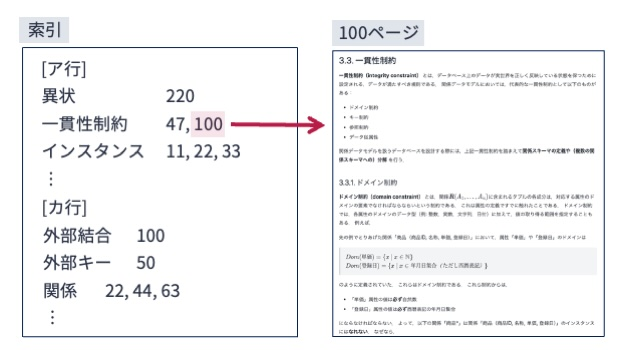
\includegraphics[width=1.0\textwidth]{figure/indexing/book-index.jpg}
    \caption{書籍における索引の例}
    \label{fig:book-index}
\end{figure}

データベースにおける索引も書籍のそれと類似した役割をもちます．
データベースにおける\strong{索引（インデックス; index）}とは，データベース中のある属性に注目し，ある属性値を持つレコードを効率よく取得できるよう工夫された特殊なデータです．
索引は
\begin{itemize}
\item \strong{索引キー（index key）}と呼ばれる検索対象となる属性の値，および
\item その値をもつレコードの場所を特定する情報（記憶装置の中でレコードが格納されている場所）
\end{itemize}
から構成されます．

図\ref{fig:db-index}は「商品」テーブルの属性「単価」に関する索引，およびそれを利用した問い合わせのイメージです．
「単価」の索引には，単価の値（索引キー）とその値をもつレコードが格納された場所のペアが記載されています．
この索引を使えば，ある属性値をもつレコードが格納されている場所をすぐに知ることができるため，条件に合致するレコードを効率よく取得することができます．
例えば，単価の値が\graybox{230}のレコードを検索したい場合を考えましょう．
まずは索引を上から調べていき，\graybox{230}の値がどこにあるかを調べます．
図の例では，\graybox{230}の値を持つレコードの場所は\graybox{2}であることが分かります．
場所が分かれば，指定された記憶装置の場所（アドレス\graybox{2}）を調べに行くことで欲しいレコードの情報を得ることができます．
\begin{figure}[tb]
    \centering
    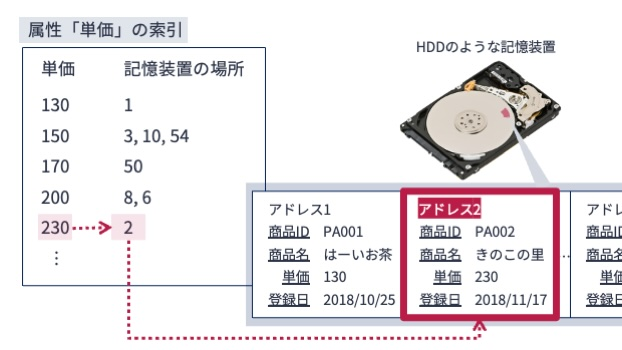
\includegraphics[width=1.0\textwidth]{figure/indexing/db-index.jpg}
    \caption{データベースにおける索引の例}
    \label{fig:db-index}
\end{figure}

書籍における索引は「わざわざ」本の末尾に索引用ページ（場所）を作っています．
それと同様，データベースの索引についても「わざわざ」記憶装置の場所（空間）を消費して索引用データを作っています．
索引は\strong{空間効率を犠牲にして時間効率を向上させる方法}です．
空間効率の劣化を抑えつつ時間効率を向上させるために，様々な種類の索引が提案されています．


\section{二分探索}
例えば，格納されたレコード数が10万のテーブルに対して，ある属性に関する索引を構築したとしましょう．
索引のサイズ（索引キーの数）が索引付けの対象となるレコード数の5分の1になった場合，索引リストの先頭から索引キーの値を一つ一つ調べていく線形探索を行うと，最悪2万回もの確認が必要となります．
索引を使えば，特定の条件を満たすレコードが探しやすくなる -- 直感的にはその通りなのですが，索引（キーのリスト）も巨大になってしまうと，そこから条件に合致する箇所を探すのにも効率の良い方法が必要となります．

索引キーがソートされている場合には，索引の探索効率を劇的に向上させる方法として二分探索が使えます．
\strong{二分探索（binary search）}は，ソート済みの配列から指定した値を高速に探索するアルゴリズムです．
二分探索アルゴリズムの概要は以下の通りです：
\begin{enumerate}
\item 配列のちょうど真ん中の位置の値をチェックする．チェックした値が探している値の場合，そこで終了
\item チェックした値が探している値よりも
    \begin{itemize}
    \item 「小さかった」場合，配列の「右半分」を新たな検索対象配列とする
    \item 「大きかった」場合，配列の「左半分」を新たな検索対象配列とする
    \end{itemize}
\item 値が見つかるまで，ステップ1-2を繰り返す．配列の長さが1になっても見つからなかったら，探している値は配列にはなかったことになる
\end{enumerate}

図\ref{fig:binary-search}を使って，二分探索の振る舞いを確認してみましょう．
図の一番上には，ソートされた索引キーの配列が並んでいます．
配列の位置は索引における行番号と考えてください．
今，\graybox{270}という値（をもつレコード）の場所がどこかを知りたいとしましょう．
配列の先頭から愚直に調べていくと，\graybox{270}の値が入った場所を見つけるには計5回の確認が必要となります．

一方，二分探索を適用すると，以下のような手順で値の場所が見つかります．
\begin{figure}[tb]
    \centering
    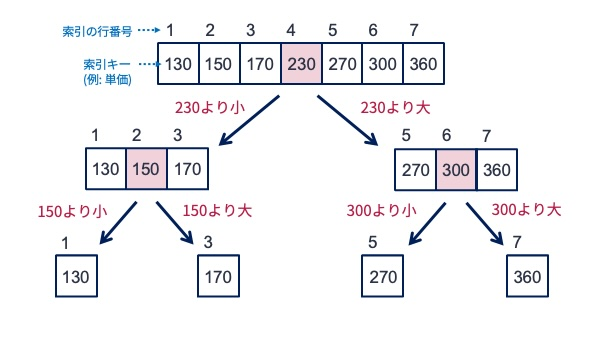
\includegraphics[width=1.0\textwidth]{figure/indexing/binary-search.jpg}
    \caption{二分探索のイメージ}
    \label{fig:binary-search}
\end{figure}
\begin{enumerate}
\item まず配列の真ん中である4番目にアクセスし値を見る（値=\graybox{230}）
\item 所望の値である\graybox{270}は\graybox{230}より大きいので，右半分の配列の真ん中の位置（6番目）にアクセスする（値=\graybox{300}）
\item 所望の値である\graybox{270}は\graybox{300}より小さいので，先ほど確認した配列の左半分の真ん中（5番目しかない）にアクセスする
\item 値が\graybox{270}であったので，位置情報として\graybox{5}を返す（終了して，索引の5行目に記されている記憶装置の場所にあるレコードを調べに行く）
\end{enumerate}

\graybox{270}の値を見つけるのに要した配列へのアクセス回数は合計3回となります．
二分探索では，1ステップごとに調査対象となる配列のサイズが半分になります．
そのため，もとの配列のサイズが$N$のとき，所望の値を見つけるために必要となる配列へのアクセス回数は最悪のケースでも$\log_2 N$回となります．
図\ref{fig:binary-search}の例では配列のサイズが小さいため二分探索の効果が感じにくいですが，配列のサイズが巨大になると二分探索の効果が実感できます．
例えば索引のサイズ（索引キーの種類数）が100万の場合，二分探索を使えば索引キーの配列に20回（$\log_2 10^6$回）程度アクセスするだけで所望の値を見つけることができます．


\section{B+木}
二分探索はソート済み配列を探索する上で強力な方法ですが，データベースの索引キーの探索に使うには以下のような欠点があります．
\begin{itemize}
\item データベースが超巨大になると索引のサイズも超巨大になるため，さすがの二分探索も遅くなる\footnote{索引データが大きすぎると高速なメモリに収まりきらないため，動作の遅いディスク（補助記憶装置）に配置することになります．二分探索はデータ全体をあちこち飛び飛びに確認しますが，ディスクのような補助記憶装置では読み取り操作が遅く，そのような操作が何度も発生してしまうと，それが検索スピードの足かせとなってしまいます．}
\item 属性値がある範囲の値をもつレコードを探索したいというケースにおいて，単一の値の検索に特化した二分探索は分が悪い
\item データベースではレコードの追加や更新が頻繁に発生するため，データベースの更新ごとに巨大な索引キーをソートするのは効率が悪い（定番のソートアルゴリズム「クイックソート」を使っても$O(N \log N)$の計算時間がかかる）
\end{itemize}

\strong{B+木（B+ tree）}\footnote{諸説ありますが，データベースの教科書として著名な``Principles of Database Systems (Jeffrey Ullman著)''によると，B+木の``B''はbalancedの頭文字に由来しています．}は，二分探索よりも高速かつ効率よくデータの探索を行え，かつ更新にかかるコストも小さい，データベース索引用のデータ構造です\cite{Knuth本}．
索引のリストが巨大になっても高速に探索できるよう，B+木は索引を階層的に管理することで，二分探索の欠点を克服しています．
B+木は以下のような特徴を持つ木構造データです（$d$および$e$の値は事前に決めておく）．
\begin{enumerate}
\item 根ノードから葉ノードへのパスの長さはすべて同じである
\item 葉ノードは索引キーの（順序付き）集合で構成される．各葉ノードは索引キーを収容するスペースをもつ．そのスペースには最小$\lceil \frac{e}{2} \rceil$個，最大$e$個の索引キーを収容できる．なお，葉ノード中の索引キーは昇順にソートされている
\item 隣接する葉ノードはリンクで結ばれている（すぐ隣の索引キーが何か分かる）
\item 葉ノード以外のノードは，ポインタと探索キーを交互に持つ．なお，ノードに収容できるポインタの数は最大で$2d+1$個，探索キーは最大$2d$個である．探索キー$k$の左隣のポインタは値が$k$未満の探索キーを含む子ノードにリンクしている．探索キー$k$の右隣のポインタは値が$k$以上の探索キーを含む子ノードにリンクしている
\item 根ノードは1個以上の探索キーを持つ
\item 根ノード，葉ノード以外の中間ノードは$d$個以上の探索キーを持つ
\item 葉ノードの各索引キーはその値を属性値としてもつレコード集合とリンクしている（記憶装置で該当レコードが記録されている位置にすぐ飛べる）
\end{enumerate}
なお，$d$の値をB+木の\strong{次数}と呼びます．

上の定義だけでは分かりづらいので，図\ref{fig:b+tree}を見ながらB+木の特徴を確認しましょう．
ある属性$A$の索引キー（属性値）として
\begin{equation*}
1, 4, 9, 16, 25, 36, 49, 64, 81, 100, 121, 144,169, 196, 225, 256
\end{equation*}
のいずれかを取るレコードを格納したテーブルがあるとします．
図\ref{fig:b+tree}は，このテーブルの属性$A$に関するB+木です．
なお，このB+木は$d=1，e=3$としています．
\begin{figure}[tb]
    \centering
    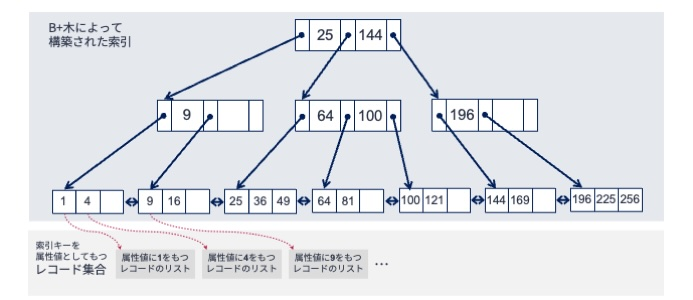
\includegraphics[width=1.0\textwidth]{figure/indexing/b+tree.jpg}
    \caption{属性$A$に関するB+木の例（$d=1, e=3$）}
    \label{fig:b+tree}
\end{figure}

図を見たら分かるように，すべての索引キーはいずれかの葉ノードに格納されています（特徴2）．
索引キーが格納されたどの葉ノードについても，根ノードから2回枝をたどるだけで到達できます（特徴1）．
また，根以外のどのノードも半数以上スペースが埋まっています（特徴2および6）．
さらに，ある索引キーの次に小さい（大きい）索引キーは同じ葉ノード内で隣接している，もしくは隣接する葉ノード内に存在しています（特徴3）．
そのため，例えば索引キーの\graybox{4}の次に大きい索引キーを知りたければ，\graybox{4}が含まれる一番左の葉ノードから右隣にリンクされている葉ノードを見ることで，\graybox{9}が次に大きい索引キーであることが分かります．

B+木において，葉ノードは，各レコードの格納場所情報を保持しているため，いわゆる索引と見なすことができます．
一方，葉ノードの親ノードは，葉ノードを振り分け，葉ノードの場所を管理しているという意味では，\strong{索引の索引}になっていると見なせます．
このように，B+木は索引を階層的に管理します．


B+木で重要なことは，どの葉ノードも\strong{根ノードからの距離が同じ}であることです．
この設計によって，どの索引キーも同じ計算時間で見つけることができます．
一方，どのノードも常に\strong{半数以上}スペースが埋まっているという特徴は，裏を返せば半分は空いていてもよいということになります．
これは索引に割り当てる記憶領域が無駄になっていると言えますが，空きがあれば木の構造を大きく変えずに新たな索引キーが挿入できるため，索引更新に柔軟性を持たせる工夫とも言えます．
このようなB+木を索引に使うことで，ある条件にマッチするレコードを高速に探索することができます．
また，レコードが追加・更新・修正されても，コストを抑えて索引を更新することができます．

以下では，B+木を用いたレコードの探索方法について見てみましょう．


\subsection{B+木を用いたレコードの探索}
ある属性値をもつレコードの探索は，ノードに含まれる探索キーをチェックしながらB+木の根ノードから葉ノードまでたどることで行います．
例えば，ある属性$A$の値として，
\begin{equation*}
1, 4, 9, 16, 25, 36, 49, 64, 81, 100, 121, 144,169, 196, 225, 256
\end{equation*}
のいずれかを取るレコードが格納された関係表に対して，B+木による索引を構築したとしましょう．
図\ref{fig:b+tree}はこの例におけるB+木となっています．

このB+木を使って，属性$A$の値が\graybox{121}となるレコードを探すことを考えましょう．
手順は以下の通りとなります（図\ref{fig:b+tree-search}も参照すること）．
\begin{figure}[tb]
    \centering
    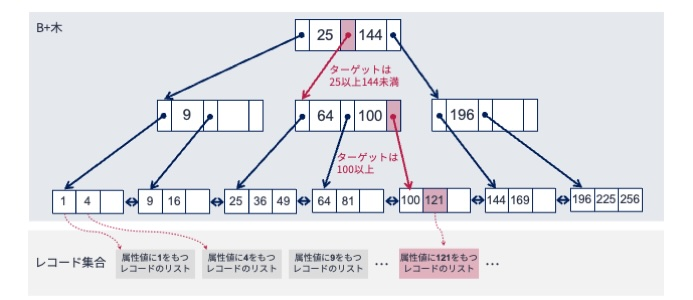
\includegraphics[width=1.0\textwidth]{figure/indexing/b+tree-search.jpg}
    \caption{B+木を用いたレコード探索のイメージ}
    \label{fig:b+tree-search}
\end{figure}

まず，根ノードにアクセスし格納された探索キーを調べます．
探索キーは\graybox{25}と\graybox{144}です．
ターゲットとなる値は\graybox{121}であり，\graybox{25}よりも大きく\graybox{144}よりも小さいです．
よって，探索キー\graybox{25}と\graybox{144}の間にあるポインタをたどります．
ポインタをたどった先にあるノードには，探索キーとして\graybox{64}と\graybox{100}が格納されています．
先ほどと同様，ターゲットとなる値と探索キーの関係を調べると，ターゲット値である\graybox{121}は\graybox{100}より大きいです．
よって，探索キー\graybox{100}の右隣にあるポインタをたどります．
その結果，葉ノードにたどり着きます．
葉ノードに格納された索引キーを左から右に探索すると，左から2番目にターゲット値である索引キー\graybox{121}が見つかります．
所望の索引キーが見つかったので，索引キーからリンクされたレコードを取得します．
これにて探索完了です．

B+木の特徴6に記した条件により，根を除くどの中間ノードも子ノードを少なくとも$d+1$個持つことが保証されています．
これにより，索引キーの総数が$N$の場合，B+木の根ノードから葉ノードへのパスの長さ（木の高さ）は高々$O(\log_{d+1} N)$となります．
各ノード内には最大$2d$個の探索キーがあり，これらをチェックする手間はかかります．
しかし，データベースの探索において真に時間がかかるのは「ディスクからノードをメモリに読み込む処理（ディスクI/O）」です．
B+木を用いた探索では，この非常に重いディスク読み取りの回数がパスの長さと同じ$O(\log_{d+1} N)$回で済むため，膨大なデータに対しても極めて高速な探索が保証されるのです．


\subsection{範囲探索}
B+木を使えば，範囲探索も容易に行えます．
先ほどの例で使ったB+木を使って，属性値がある範囲にあるレコードを探索する手順を示しましょう．

今，属性値が\graybox{10}以上\graybox{40}未満であるレコードをすべて取得したいとします．
手順は以下の通りです（図\ref{fig:range-search}も参照すること）．
\begin{figure}[tb]
    \centering
    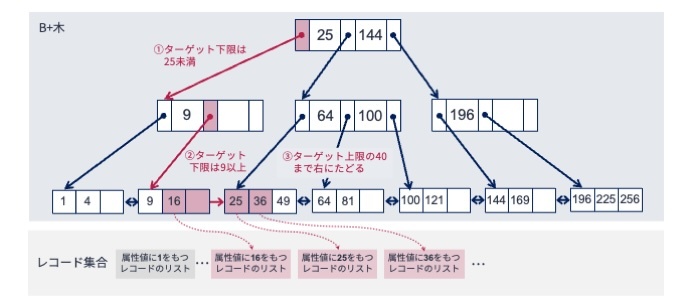
\includegraphics[width=1.0\textwidth]{figure/indexing/range-search.jpg}
    \caption{B+木を用いた範囲探索のイメージ}
    \label{fig:range-search}
\end{figure}

探索条件の下限である\graybox{10}に着目します．
まず根ノードにアクセスし，格納された探索キーを調べます．
探索キーは\graybox{25}と\graybox{144}です．
ターゲットとなる値は\graybox{10}であり，\graybox{25}よりも小さいです．
よって，探索キー\graybox{25}の左にあるポインタをたどります．
ポインタをたどった先にあるノードには，探索キーとして\graybox{9}が格納されています．
ターゲット値は\graybox{10}であるため，探索キー\graybox{9}の右隣にあるポインタをたどります．
その結果，葉ノードにたどり着きます．

葉ノードに格納された索引キーを左から探索すると，左から2番目にターゲット値である\graybox{10}より大きい索引キー\graybox{16}が見つかります．
ところで，ターゲットとなる属性値の上限は\graybox{40}でした．
そこで，先ほど見つけた索引キー\graybox{16}から右側にリンクをたどりながら索引キーが\graybox{40}未満のものをすべて拾い上げていきます．
すると，索引キーとして\graybox{16，25，36}が見つかります．
条件を満たす索引キーがすべて見つかったので，各索引キーからリンクされたレコードを取得します．
これにて範囲探索完了です．


\subsection{B+木の構築・更新}
すでに述べたように，データベースではレコードの追加や更新が度々行われます．
そのため，データベースの更新に応じて索引の更新も必要となります．

B+木は根ノードから葉ノードへのパスの長さが均一になるよう（木の高さのバランスを崩さない）よう，索引を更新するアルゴリズムが提案されています．
直感的には，
\begin{itemize}
\item 新たな索引キーを挿入する場合には，木の構造を崩して木を上に向かって伸ばす
\item 索引キーを削除する場合には，キーの挿入操作の逆を行う
\end{itemize}
といった戦略でB+木を更新します．
B+木の更新アルゴリズムの詳細については「IT Text データベースの基礎\cite{吉川本}」「データベースシステム（改訂2版）\cite{北川本}」「リレーショナルデータベース入門（第3版）\cite{増永本}」などの良書を参照してください．


\section{ハッシュ索引}
B+木のような木構造の索引では，根ノードから葉ノードにまでたどることで，条件にマッチする属性値をもつレコードが格納されている場所を調べます．
探索を容易にするためにB+木では索引を木構造にする工夫をこらしていますが，$O(\log_m{N})$の計算時間をかけて根から葉に向かって木をたどらなければなりません．

仮に，ある値が指定されたときにそれを属性値としてもつレコードの格納位置を「直接」知ることができれば，B+木よりももっとカンタンに求めるレコードを取得することができます．
これを実現するのが，\strong{ハッシュ索引（hash index）} です\cite{Fagin1979, Litwin1980}．
B+木と同様，ハッシュ索引も探索対象となる属性を指定して索引を構築します．

B+木と異なるのは，ハッシュ索引では索引キーの値とレコード（の格納場所）との対応付けを行うために\strong{ハッシュ関数（hash function）} を用いる点です．
ハッシュ関数とは，任意の値を別の都合の良い値（ハッシュ値）に変換するための関数です．
良いハッシュ関数は値の変換にかかる計算コストが低くなるよう設計されています．

$mod_d(x)$は，整数$x$を整数$d$で割ったときの剰余（いわゆる余り）を計算する関数です．
ただし$q$は整数とします．
\begin{equation*}
mod_d(x) = r  \quad \text{where} \,\, x = q \cdot d + r
\end{equation*}
剰余演算は高速に実行できることが知られており，ハッシュ索引を構築するためのハッシュ関数としてしばしば使われます．
例えば，学生情報を格納するテーブル\graybox{学生}に対して，属性\graybox{学籍番号}の値を探索キーとするハッシュ索引を構築するとしましょう．
一般に学籍番号は数字以外の文字も含まれる文字列ですが，計算機の中では文字列も整数値で表現されているので，剰余を計算することは可能です．
そこで，図\ref{fig:hash-index}のように\graybox{学生}テーブルの各レコードの\graybox{学籍番号}の値に剰余を計算する関数を適用し，得られた剰余値が示す記憶装置の場所にレコードを格納します．
イメージとしては，$d＝100$の場合，「学籍番号の下2桁」だけを見て，レコードをどこの場所にしまうかを決める，ということをします．
このようにハッシュ索引を構築しておけば，レコードを取得したい学生の学籍番号から剰余値を1回計算するだけで，必要となる学生情報が格納されている場所を特定し，レコードを取得することができます．
\begin{figure}[tb]
    \centering
    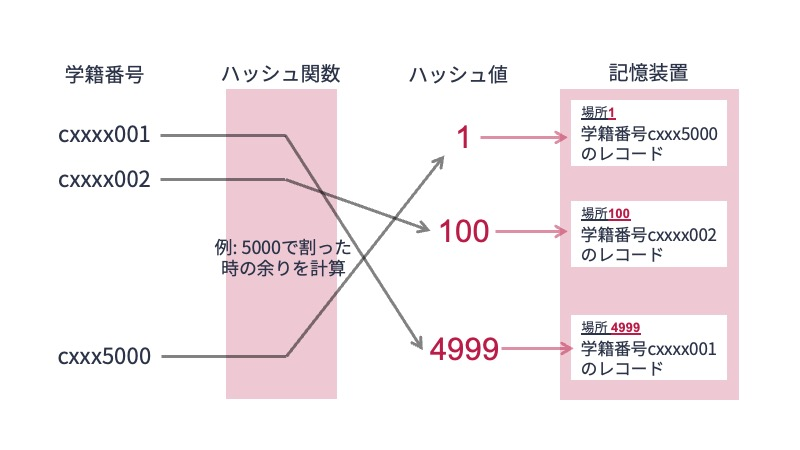
\includegraphics[width=1.0\textwidth]{figure/indexing/hash-index.jpg}
    \caption{ハッシュ索引のイメージ}
    \label{fig:hash-index}
\end{figure}

高速にレコードを取得できるハッシュ索引ですが，致命的な弱点があります．
ハッシュ索引は，各レコードの属性値のハッシュ値に対応するレコードの格納場所を直接割り出しており，探索キーの値が完全一致するものしか見つけられません．
そのため，範囲探索が必要な属性に対しては，B+木のような索引を用いる必要があります．


\section{SQLによる索引の構築}
代表的な索引づけ方法を紹介しましたので，最後に索引を構築するためのSQL文を見ておきましょう．
大抵の関係データベース管理システムでは，コード\ref{code:sql-create-index-structure}のようなSQL文で，テーブルの特定の属性に対して索引を構築することができます（「インデックスを張る」ともいう）．
\begin{figure}[h]
    \begin{minted}[gobble=1,
        bgcolor=background,
        fontsize=\small,
        linenos=false,
        xleftmargin=0em]{sql}

    CREATE INDEX インデックス名
        ON テーブル名 (索引の対象となる属性名)
    USING 索引種別;

    \end{minted}
    \captionsetup{name=コード}
    \caption{索引構築のためのSQLの構文}
    \label{code:sql-create-index-structure}
\end{figure}

例えば\graybox{product}テーブルの属性\graybox{price}に関してB+木を使った索引を構築したい場合は，コード\ref{code:sql-create-btree-index}のようなSQL文を使います．
\begin{figure}[h]
    \begin{minted}[gobble=1,
        bgcolor=background,
        fontsize=\small,
        linenos=false,
        xleftmargin=0em]{sql}

    CREATE INDEX product_price_idx
        ON product (price)
    USING btree;

    \end{minted}
    \captionsetup{name=コード}
    \caption{B+木を使った索引を構築するためのSQL文}
    \label{code:sql-create-btree-index}
\end{figure}

一般に，主キーや外部キーとして指定された属性には自動的に索引が構築されますが，それ以外の属性に索引を構築したい場合は上記のようなSQL文を発行する必要があります．
問い合わせに対する応答速度が遅い場合，索引の構築は非常に効果的です．
一方，索引は記憶領域を余分に消費するので，無闇に索引を構築するのは避けるべきです．



% ---------------------------------------
\section{クイズ}
% ---------------------------------------

\subsection*{Q1. B+木の探索（1/2）}
図\ref{fig:b+tree}に示されたB+木において，属性$A$の値が16であるレコードを探索する際，根ノードから順にたどる探索キー（比較対象となる値）をすべて列挙しなさい．

\subsection*{Q2. B+木の探索（2/2）}
図\ref{fig:b+tree}に示されたB+木において，範囲検索として属性$A$の値が25以上81以下のレコードを取得する場合，葉ノード（最下層）においてスキャンされる索引キーを順番にすべて答えなさい．


\subsection*{Q3. 索引づけの選択}
あるオンラインショッピングサイトのデータベースには，以下の関係スキーマを持つ「注文」テーブルがあります．
「配送ステータス」には「未発送」「発送済」「キャンセル」の3種類の値のいずれかが入ります．
このデータベースでは，主キーである「注文ID」には自動的にB+木で索引づけがなされています．
\begin{equation}
\textbf{注文}(\underline{\text{注文ID}}, \text{ユーザID}, \text{商品ID}, \text{注文日}, \text{配送ステータス})
\end{equation}

システムを運用したところ，特定の条件での検索に時間がかかっていることが判明したため，追加で索引づけすることを検討しています．
以下の候補のうち，新たに索引を構築する対象として最も不適切なものはどれでしょうか．
その理由とともに答えなさい．

\begin{itemize}
\item 注文ID
\item ユーザID（ある特定のユーザの注文履歴を一覧表示する処理が頻繁に実行される）
\item 注文日（ある特定の日付の売り上げを集計する処理が頻繁に実行される）
\item 配送ステータス（まだ発送されていない注文を絞り込む処理が実行される）
\end{itemize}


\subsection*{Q4. 索引づけとトレードオフ}
企業の社員情報を管理する，以下の関係スキーマを持つ「社員」テーブルがあります．
\begin{equation}
\textbf{社員}(\underline{\text{社員ID}}, \text{氏名}, \text{部署名}, \text{入社年度}, \text{給与})
\end{equation}

このデータベースに対して，以下の2種類の問い合わせが非常に高い頻度で実行されることが分かりました．
\begin{itemize}
    \item 特定の部署に所属する社員の一覧を取得する（例: \graybox{WHERE 部署名 = `営業部'}）
    \item 特定の入社年度の社員の一覧を取得する（例: \graybox{WHERE 入社年度 = 2020}）
\end{itemize}
一方で，この会社では毎月多くの新入社員や中途社員が入社するため，「社員」テーブルに対するレコードの追加も頻繁に行われます．

属性「部署名」と「入社年度」のそれぞれに索引づけを行うべきでしょうか．
索引を構築することによるメリット（検索速度の向上）とデメリット（更新コストの増加など）のトレードオフを踏まえ，あなたの考えを説明しなさい．


\backmatter
\bibliography{reference}
\bibliographystyle{tipsj}

\end{document}
